\documentclass[a4paper]{scrartcl}

\usepackage[
fancytheorems,
fancyproofs,
noindent
]{adam}

\usepackage{tikz}
\usepackage{booktabs}
\usepackage{mathtools}
\usetikzlibrary{decorations.pathreplacing, arrows.meta, calc}

\title{Representation Theory}
\author{Adam Kelly (\texttt{ak2316@cam.ac.uk})}
\date{\today}

% Course-specific macros
\newcommand{\U}{\operatorname{U}}
\newcommand{\SU}{\operatorname{SU}}
\newcommand{\Hom}{\operatorname{Hom}}
\newcommand{\End}{\operatorname{End}}
\newcommand{\Ind}{\operatorname{Ind}}
\newcommand{\Res}{\operatorname{Res}}
\newcommand{\Irr}{\operatorname{Irr}}
\newcommand{\id}{\operatorname{id}}
\newcommand{\rank}{\operatorname{rank}}
\newcommand{\Cent}{\operatorname{C}}
\newcommand{\Symm}{\operatorname{S}}
\newcommand{\ip}[2]{\langle #1, #2 \rangle}
\newcommand{\gen}[1]{\langle #1 \rangle}
\newcommand{\HH}{\mathbb{H}}

\allowdisplaybreaks

\begin{document}

\maketitle

Groups are, in the end, a way of talking about symmetry. But a group presented abstractly -- as a set with a multiplication table, or as generators and relations -- is a slippery thing to get hold of. Representation theory takes the view that the way to understand a group is to watch it \emph{act}, and the most tractable things a group can act on are vector spaces. A representation is exactly that: a group acting by invertible linear maps. Once we are in the world of linear algebra we can bring the whole toolbox -- eigenvalues, traces, direct sums, tensor products -- to bear on questions that started out being about groups.

The astonishing thing, and the thing that makes this course so satisfying, is how much information survives when we throw away almost everything. To each representation we attach its \vocab{character}, a single complex-valued function on the group recording only the trace of each group element. This looks like a hopeless loss of information, and yet over $\C$ the character determines the representation completely. The characters of the irreducible representations satisfy beautiful orthogonality relations, they can be assembled into a finite square array called the character table, and that little table encodes a remarkable amount about the group. We will use it to prove Burnside's theorem, that every group of order $p^a q^b$ is soluble -- a purely group-theoretic statement for which no purely group-theoretic proof was known for decades.

This article constitutes my notes for the `Representation Theory' course, held in Michaelmas 2021 at Cambridge. These notes are \emph{not a transcription of the lectures}, and differ significantly in quite a few areas. Still, all lectured material should be covered.

\tableofcontents

\clearpage

\section{Representations}

\subsection{Some Preliminaries}

Before we begin properly, it is worth being clear about what we are assuming, since this course sits right on top of \emph{Linear Algebra} and \emph{Groups, Rings and Modules}.

Throughout, `vector space' means a \emph{finite dimensional} vector space unless we say otherwise. Our base field will be written $F$ or $k$, and although a fair amount of what we do works over any field, the theory only becomes really clean when $F$ is algebraically closed of characteristic zero. So the reader should keep $F = \C$ firmly in mind: essentially every theorem with any content in this course is a theorem about complex representations.

Recall from linear algebra that if $V$ is a vector space over $F$, then
$$\GL(V) = \{ \alpha : V \to V \mid \alpha \text{ is linear and invertible}\}$$
is a group under composition, the \vocab{general linear group} of $V$. If $\dim V = n$ then a choice of basis $e_1, \dots, e_n$ identifies $V$ with $F^n$ and hence identifies $\GL(V)$ with the group $\GL_n(F)$ of invertible $n \times n$ matrices over $F$. Changing basis changes the identification by conjugation: if $\alpha$ has matrix $A$ in one basis and $A'$ in another, then $A' = P^{-1} A P$ for the change of basis matrix $P$. This is worth saying out loud now, because \emph{everything} in this course is invariant under conjugation, and that is not a coincidence.

We will need one more piece of linear algebra constantly.

\begin{proposition}[Diagonalisability]
	Let $\alpha \in \GL(V)$ with $V$ a finite dimensional $\C$-vector space, and suppose $\alpha^m = \id$ for some $m \geq 1$. Then $\alpha$ is diagonalisable.
\end{proposition}
\begin{proof}
	The polynomial $X^m - 1$ annihilates $\alpha$, and over $\C$ it factors as $\prod_{j=0}^{m-1}(X - \omega^j)$ where $\omega = e^{2\pi i/m}$, which has no repeated roots. A linear map is diagonalisable if and only if its minimal polynomial splits into distinct linear factors, and the minimal polynomial divides $X^m - 1$, so we are done.
\end{proof}

In particular, if $g$ is an element of a finite group and $\alpha$ is the linear map by which $g$ acts, then $\alpha$ is diagonalisable, with eigenvalues roots of unity. This single observation is responsible for a surprising amount of what follows.

There is also a version for several maps at once, whose proof the reader has essentially seen in \emph{Linear Algebra} when simultaneously diagonalising commuting operators.

\begin{proposition}[Simultaneous diagonalisation]
	Let $\alpha, \beta \in \GL(V)$ be diagonalisable, with $V$ a $\C$-vector space. If $\alpha\beta = \beta\alpha$, then there is a basis of $V$ in which $\alpha$ and $\beta$ are both diagonal.
\end{proposition}
\begin{proof}
	Write $V = \bigoplus_{\lambda} V_\lambda$ as a sum of eigenspaces of $\alpha$. If $v \in V_\lambda$ then $\alpha(\beta v) = \beta(\alpha v) = \lambda \beta v$, so $\beta$ preserves each $V_\lambda$. Now $\beta|_{V_\lambda}$ is diagonalisable (its minimal polynomial divides that of $\beta$, which has distinct linear factors), so pick an eigenbasis of $\beta$ on each $V_\lambda$ and put them together.
\end{proof}

On the group theory side, recall that an \vocab{action} of a group $G$ on a set $X$ is a map $G \times X \to X$, written $(g, x) \mapsto g \cdot x$, satisfying $e \cdot x = x$ and $g\cdot(h \cdot x) = (gh)\cdot x$. Equivalently -- and this is the point of view we want -- an action of $G$ on $X$ is precisely a group homomorphism $G \to \sym(X)$, the group of all bijections $X \to X$.

Recall also that the \vocab{conjugacy class} of $g \in G$ is
$$\ccl_G(g) = \{ x g x^{-1} \mid x \in G \},$$
that these classes partition $G$, and that by the orbit--stabiliser theorem $|\ccl_G(g)| = |G : \Cent_G(g)|$ where $\Cent_G(g) = \{x \in G \mid xg = gx\}$ is the centraliser. Conjugacy classes will play the role for us that `points' play elsewhere, so here is a picture to fix ideas.

\begin{center}
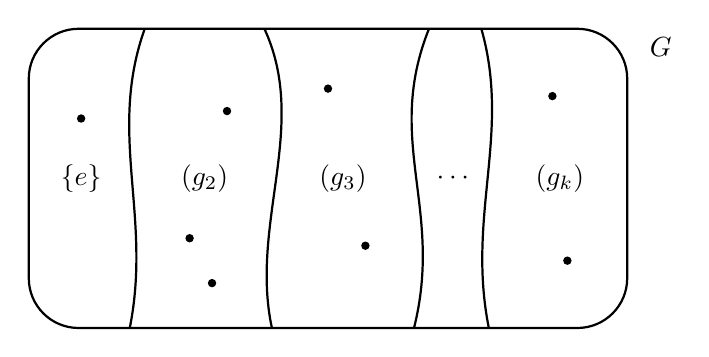
\begin{tikzpicture}[scale=0.95]
	\draw[rounded corners=18pt, thick] (0,0) rectangle (8,4);
	\node at (8.45,3.75) {$G$};
	% partition into classes
	\draw[thick] (1.35,0) .. controls (1.65,1.5) and (1.05,2.6) .. (1.55,4);
	\draw[thick] (3.25,0) .. controls (2.95,1.4) and (3.75,2.7) .. (3.15,4);
	\draw[thick] (5.15,0) .. controls (5.55,1.6) and (4.75,2.5) .. (5.35,4);
	\draw[thick] (6.15,0) .. controls (5.85,1.5) and (6.45,2.6) .. (6.05,4);
	\node at (0.7,2) {$\{e\}$};
	\node at (2.35,2) {$\ccl(g_2)$};
	\node at (4.2,2) {$\ccl(g_3)$};
	\node at (5.7,2) {$\cdots$};
	\node at (7.1,2) {$\ccl(g_k)$};
	\fill (0.7,2.8) circle (1.6pt);
	\fill (2.15,1.2) circle (1.6pt);
	\fill (2.65,2.9) circle (1.6pt);
	\fill (2.45,0.6) circle (1.6pt);
	\fill (4.0,3.2) circle (1.6pt);
	\fill (4.5,1.1) circle (1.6pt);
	\fill (7.0,3.1) circle (1.6pt);
	\fill (7.2,0.9) circle (1.6pt);
\end{tikzpicture}
\end{center}

The moral of the course, stated far too early, is that the natural `coordinates' on a group are indexed by its conjugacy classes, and the natural `functions' in those coordinates are the irreducible characters. There will be exactly as many of the latter as the former.

\subsection{Definitions and First Examples}

We now come to the central definition. Since an action of $G$ on a set is a homomorphism into $\sym(X)$, and since a vector space is a set with extra structure, the right thing to do is to replace $\sym$ by $\GL$.

\begin{definition}[Representation]
	Let $G$ be a group and $V$ a vector space over $F$. A \vocab{representation} of $G$ on $V$ is a group homomorphism
	$$\rho : G \to \GL(V).$$
	We call $V$ the \vocab{representation space}, and we write the representation as the pair $(\rho, V)$, or often just as $\rho$ or just as $V$ when the rest is clear.
\end{definition}

Unwinding the definition of homomorphism, giving a representation is the same as giving, for each $g \in G$, a linear map $\rho(g) : V \to V$ such that $\rho(e) = \id_V$ and $\rho(gh) = \rho(g)\rho(h)$ for all $g,h \in G$. Note that invertibility comes for free from these two conditions, since $\rho(g)\rho(g^{-1}) = \rho(e) = \id_V$; so we may as well only ask for linear maps.

\begin{definition}[Degree]
	The \vocab{degree} (or \vocab{dimension}) of a representation $(\rho, V)$ is $\dim_F V$.
\end{definition}

\begin{definition}[Faithful representation]
	A representation $\rho$ is \vocab{faithful} if $\kernel \rho = \{e\}$, i.e. if $\rho$ is injective.
\end{definition}

A faithful representation realises $G$ concretely as a group of matrices, which is often exactly what one wants. Non-faithful representations are not a defect, though; they are how the theory sees the normal subgroups of $G$.

Everything is much clearer with examples, so let us collect a good supply now. Almost all of these will reappear repeatedly.

\begin{example}[The trivial representation]
	For any group $G$ and any vector space $V$, the map $\rho(g) = \id_V$ for all $g$ is a representation. When $V = F$ is one dimensional this is called \vocab{the} trivial representation, and we write it $\mathbf{1}$ or $\mathbf{1}_G$. It is faithful only when $G$ is trivial.
\end{example}

\begin{example}[Representations of a cyclic group]
	Let $G = C_m = \gen{g}$ be cyclic of order $m$, and let $V$ be a $\C$-vector space. A representation of $G$ is determined by $\alpha = \rho(g) \in \GL(V)$, and the only constraint is $\alpha^m = \id$. So representations of $C_m$ on $V$ correspond exactly to elements of $\GL(V)$ of order dividing $m$.

	By our proposition above, such an $\alpha$ is diagonalisable, so there is a basis in which
	$$\rho(g) = \begin{pmatrix} \omega^{a_1} & & \\ & \ddots & \\ & & \omega^{a_n}\end{pmatrix}, \qquad \omega = e^{2\pi i /m}$$
	for some $a_1, \dots, a_n$. So every representation of $C_m$ breaks up into one-dimensional pieces $g \mapsto \omega^{a}$. We will see this is a special case of a general theorem.
\end{example}

\begin{example}[Dihedral groups]
	Let $D_{2n} = \gen{r, s \mid r^n = s^2 = e, \; srs^{-1} = r^{-1}}$ be the symmetry group of a regular $n$-gon. There is an obvious representation on $\R^2$ (and hence on $\C^2$): let $r$ act by rotation through $2\pi/n$ and $s$ by reflection in the $x$-axis, so
	$$\rho(r) = \begin{pmatrix} \cos \tfrac{2\pi}{n} & -\sin\tfrac{2\pi}{n} \\[2pt] \sin\tfrac{2\pi}{n} & \cos \tfrac{2\pi}{n}\end{pmatrix}, \qquad \rho(s) = \begin{pmatrix} 1 & 0 \\ 0 & -1 \end{pmatrix}.$$
	One checks the relations hold, and $\rho$ is faithful. This is the representation you should picture whenever $D_{2n}$ comes up.
	\begin{center}
	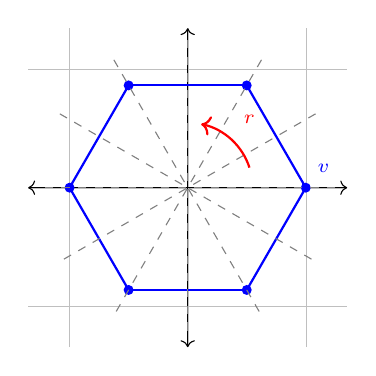
\begin{tikzpicture}[scale=1.5]
		\draw[ultra thin, color=lightgray] (-1.35,-1.35) grid (1.35,1.35);
		\draw[<->] (-1.35,0) -- (1.35,0);
		\draw[<->] (0,-1.35) -- (0,1.35);
		% hexagon
		\foreach \i in {0,...,5} {
			\pgfmathsetmacro{\a}{60*\i}
			\pgfmathsetmacro{\b}{60*(\i+1)}
			\draw[thick, color=blue] (\a:1) -- (\b:1);
			\fill[color=blue] (\a:1) circle (1.2pt);
		}
		% reflection axes
		\foreach \i in {0,...,5} {
			\pgfmathsetmacro{\a}{30*\i}
			\draw[dashed, color=gray] (\a:1.25) -- (\a+180:1.25);
		}
		\draw[->, thick, color=red] (18:0.55) arc (18:78:0.55);
		\node[color=red] at (48:0.78) {\scriptsize $r$};
		\node[color=blue] at (1.15,0.16) {\scriptsize $v$};
	\end{tikzpicture}
	\end{center}
	The dashed lines are the $n$ axes of reflection; $r$ rotates by $2\pi/n$ and each reflection swaps the two half-planes cut out by its axis.
\end{example}

\begin{example}[Symmetric groups on the standard space]
	Let $G = S_n$ act on $V = F^n$ with basis $e_1, \dots, e_n$ by permuting coordinates:
	$$\rho(\sigma)(e_i) = e_{\sigma(i)}.$$
	Extending linearly gives a representation of degree $n$; the matrix of $\rho(\sigma)$ is the permutation matrix of $\sigma$. It is faithful.
\end{example}

\begin{example}[The sign representation]
	Let $G = S_n$ and $V = F$, with $\rho(\sigma) = \sign(\sigma)$. This is a one-dimensional representation, not faithful for $n \geq 3$ (its kernel is $A_n$).
\end{example}

Two more constructions deserve to be called out because they will be with us for the whole course.

\begin{definition}[Permutation representation]
	Let $G$ act on a finite set $X$. Let $FX$ be the $F$-vector space with basis $\{e_x \mid x \in X\}$, so $\dim FX = |X|$. Then
	$$\rho(g)\Big(\sum_{x \in X} \lambda_x e_x\Big) = \sum_{x \in X} \lambda_x e_{g \cdot x}$$
	defines a representation of $G$, the \vocab{permutation representation} associated to the action.
\end{definition}

\begin{definition}[Regular representation]
	Taking $X = G$ with $G$ acting on itself by left multiplication gives the \vocab{regular representation} of $G$, on the vector space $FG$ of dimension $|G|$.
\end{definition}

The regular representation is always faithful (if $g \neq e$ then $g \cdot e = g \neq e$, so $\rho(g) \neq \id$), which already tells us something: \emph{every} finite group has a faithful representation, so every finite group is isomorphic to a group of matrices. We will see later that $FG$ is much more than a bookkeeping device -- it contains every irreducible representation of $G$, each with multiplicity equal to its degree.

\subsection{Equivalence of Representations}

The representation of $S_3$ on $\C^3$ by permutation matrices, and the `same' representation written in a different basis, should not be counted as different. We need to say when two representations are the same.

\begin{definition}[$G$-homomorphism]
	Let $(\rho, V)$ and $(\rho', V')$ be representations of $G$ over $F$. A linear map $\varphi : V \to V'$ is a \vocab{$G$-homomorphism} (or is \vocab{$G$-linear}, or \vocab{intertwines} $\rho$ and $\rho'$) if
	$$\varphi \circ \rho(g) = \rho'(g) \circ \varphi \quad \text{for all } g \in G.$$
	We write $\Hom_G(V, V')$ for the set of all such maps.
\end{definition}

The condition says exactly that the square
\begin{center}
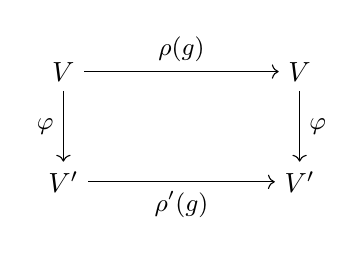
\begin{tikzpicture}[scale=1]
	\node (a) at (0,1.4) {$V$};
	\node (b) at (3,1.4) {$V$};
	\node (c) at (0,0) {$V'$};
	\node (d) at (3,0) {$V'$};
	\draw[->] (a) -- node[above] {\small $\rho(g)$} (b);
	\draw[->] (c) -- node[below] {\small $\rho'(g)$} (d);
	\draw[->] (a) -- node[left] {\small $\varphi$} (c);
	\draw[->] (b) -- node[right] {\small $\varphi$} (d);
\end{tikzpicture}
\end{center}
commutes for every $g$. Note that $\Hom_G(V,V')$ is an $F$-subspace of $\Hom_F(V,V')$, since the condition is linear in $\varphi$.

\begin{definition}[Isomorphism of representations]
	We say $(\rho, V)$ and $(\rho', V')$ are \vocab{isomorphic} (or \vocab{equivalent}), written $V \cong V'$, if there is a $G$-homomorphism $\varphi : V \to V'$ which is a linear isomorphism.
\end{definition}

If $\varphi$ is such an isomorphism then $\rho'(g) = \varphi \rho(g) \varphi^{-1}$, so at the level of matrices, isomorphism of representations of the same degree $n$ means: there is a single $P \in \GL_n(F)$ with $R'(g) = P R(g) P^{-1}$ for all $g$, where $R, R'$ are the matrix representations. In other words, isomorphism is `simultaneous change of basis'. It is straightforward to check that this is an equivalence relation.

\begin{remark}
	Note the `simultaneous' -- one matrix $P$ must work for every $g$ at once. Two representations can have $\rho(g)$ conjugate to $\rho'(g)$ for each individual $g$ and still fail to be isomorphic.
\end{remark}

\begin{example}
	Any two one-dimensional representations $\rho, \rho' : G \to \GL_1(F) = F^\times$ are isomorphic if and only if they are \emph{equal}, since $\GL_1(F)$ is abelian and conjugation does nothing.
\end{example}

\subsection{Representations as Modules}

There is a second, slicker way of packaging all this, which the reader will recognise from \emph{Groups, Rings and Modules}. It is worth setting up because it makes several later constructions obvious.

\begin{definition}[Group algebra]
	Let $G$ be a finite group and $F$ a field. The \vocab{group algebra} $FG$ is the $F$-vector space with basis $\{ g \mid g \in G\}$, that is
	$$FG = \Big\{ \sum_{g \in G} \lambda_g \, g \; \Big| \; \lambda_g \in F \Big\},$$
	equipped with the multiplication extending the group multiplication bilinearly:
	$$\Big(\sum_g \lambda_g g\Big)\Big(\sum_h \mu_h h\Big) = \sum_{g,h} \lambda_g \mu_h \, (gh).$$
\end{definition}

This makes $FG$ into a ring (indeed an $F$-algebra) of dimension $|G|$ over $F$, with identity the element $1 \cdot e$. It is commutative precisely when $G$ is abelian.

\begin{proposition}
	Let $G$ be a finite group. There is a bijective correspondence between representations of $G$ over $F$ and $FG$-modules, under which a representation $(\rho, V)$ corresponds to the module structure
	$$\Big(\sum_g \lambda_g g\Big) \cdot v = \sum_g \lambda_g\, \rho(g)(v).$$
	Under this correspondence, $G$-homomorphisms correspond to $FG$-module homomorphisms, and isomorphism of representations to isomorphism of modules.
\end{proposition}
\begin{proof}
	Given $(\rho, V)$, the displayed formula is well defined and one checks the module axioms directly: $F$-bilinearity is built in, and associativity $(ab)v = a(bv)$ reduces by bilinearity to the case $a = g$, $b = h$ basis elements, where it is $\rho(gh) = \rho(g)\rho(h)$.

	Conversely, given an $FG$-module $V$, restricting scalars along $F \hookrightarrow FG$ makes $V$ an $F$-vector space, and $\rho(g) : v \mapsto g \cdot v$ is $F$-linear with $\rho(g)\rho(g^{-1}) = \id$, so $\rho(g) \in \GL(V)$; and $\rho(gh) = \rho(g)\rho(h)$ by associativity. These two constructions are mutually inverse.

	Finally, a linear map $\varphi : V \to V'$ satisfies $\varphi(g \cdot v) = g\cdot \varphi(v)$ for all $g$ if and only if it satisfies $\varphi(a \cdot v) = a \cdot \varphi(v)$ for all $a \in FG$, by linearity.
\end{proof}

\begin{remark}
	We insist that our $FG$-modules are finite dimensional over $F$, matching our convention on representations. The regular representation is precisely $FG$ regarded as a module over itself.
\end{remark}

From now on we will use the two languages interchangeably, saying `$V$ is a $G$-space' or `$V$ is a $\C G$-module' or `$V$ is a representation of $G$' as convenient, and writing $gv$ for $\rho(g)(v)$.

\subsection{Subrepresentations and Irreducibility}

\begin{definition}[Subrepresentation]
	Let $(\rho, V)$ be a representation of $G$. A subspace $W \leq V$ is \vocab{$G$-invariant} (or is a \vocab{subrepresentation}, or a \vocab{$G$-subspace}) if $\rho(g)(W) \subseteq W$ for all $g \in G$.
\end{definition}

If $W$ is $G$-invariant then in fact $\rho(g)(W) = W$ for each $g$, since $\rho(g^{-1})(W) \subseteq W$ gives the reverse inclusion. So $\rho$ restricts to a representation $\rho|_W : G \to \GL(W)$. In module language, subrepresentations are exactly $FG$-submodules.

Every representation has the \vocab{trivial} subrepresentations $0$ and $V$. The interesting question is whether there are any others.

\begin{definition}[Irreducible]
	A representation $(\rho, V)$ is \vocab{irreducible} (or \vocab{simple}) if $V \neq 0$ and the only $G$-invariant subspaces of $V$ are $0$ and $V$.
\end{definition}

\begin{example}
	Every one-dimensional representation is irreducible, since it has no nonzero proper subspaces at all.
\end{example}

\begin{example}[The standard representation of $S_n$]
	Let $V = \C^n$ carry the permutation action of $S_n$. This is \emph{not} irreducible for $n \geq 2$: the line
	$$U = \gen{e_1 + e_2 + \cdots + e_n}$$
	is fixed pointwise by every $\sigma$, so is a subrepresentation isomorphic to the trivial representation. Its complement
	$$W = \Big\{ \sum_i \lambda_i e_i \; \Big| \; \sum_i \lambda_i = 0 \Big\}$$
	is also $G$-invariant, of dimension $n-1$; it is called the \vocab{standard representation} of $S_n$. We have $V = U \oplus W$. We will prove later (using characters, in about two lines) that $W$ is irreducible.
\end{example}

\begin{example}[A reducible but indecomposable representation]
	Irreducibility is genuinely sensitive to the ground field. Let $G = C_p = \gen{g}$ and let $F = \F_p$. Define a representation on $F^2$ by
	$$\rho(g^k) = \begin{pmatrix} 1 & k \\ 0 & 1 \end{pmatrix}.$$
	This is a homomorphism since the matrices multiply by adding the top-right entries, and $\rho(g^p) = I$ as $p \equiv 0$. The subspace $\gen{e_1}$ is invariant, so $\rho$ is reducible. But it has \emph{no} invariant complement: any invariant line would give an eigenvector of $\rho(g)$ other than a multiple of $e_1$, and $\rho(g)$ has $1$ as its only eigenvalue with a one-dimensional eigenspace.

	So over $\F_p$ things can go wrong. The next section shows that over $\C$ (or any field whose characteristic does not divide $|G|$) they never do.
\end{example}

\begin{definition}[Direct sums]
	If $(\rho_1, V_1)$ and $(\rho_2, V_2)$ are representations of $G$, their \vocab{direct sum} is the representation on $V_1 \oplus V_2$ given by $g \cdot (v_1, v_2) = (g v_1, g v_2)$. In matrix terms, choosing bases of $V_1$ and $V_2$ and concatenating,
	$$\rho(g) = \begin{pmatrix} \rho_1(g) & 0 \\ 0 & \rho_2(g)\end{pmatrix}.$$
\end{definition}

\begin{definition}[Completely reducible]
	A representation is \vocab{completely reducible} (or \vocab{semisimple}) if it is a direct sum of irreducible subrepresentations.
\end{definition}

Here is the picture to have in mind. If $V = V_1 \oplus \cdots \oplus V_k$ with each $V_i$ irreducible, then in a suitable basis every matrix $\rho(g)$ is block diagonal with blocks of sizes $\dim V_i$, \emph{simultaneously for all $g$}:

\begin{center}
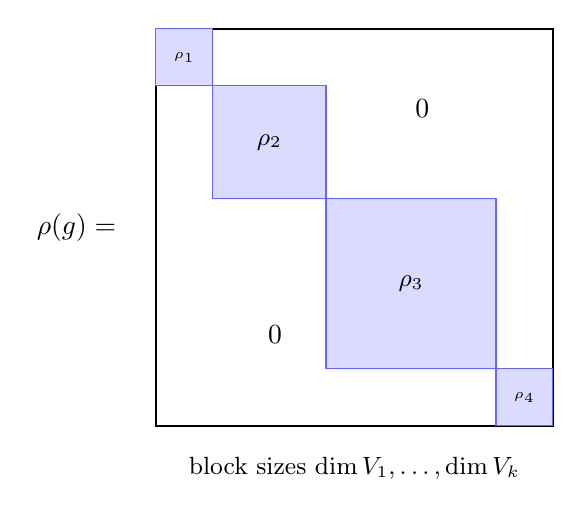
\begin{tikzpicture}[scale=0.72]
	\draw[thick] (0,0) rectangle (7,7);
	\draw[fill=blue!14, draw=blue!60] (0,6) rectangle (1,7);
	\draw[fill=blue!14, draw=blue!60] (1,4) rectangle (3,6);
	\draw[fill=blue!14, draw=blue!60] (3,1) rectangle (6,4);
	\draw[fill=blue!14, draw=blue!60] (6,0) rectangle (7,1);
	\node at (0.5,6.5) {\tiny $\rho_1$};
	\node at (2,5) {\small $\rho_2$};
	\node at (4.5,2.5) {\small $\rho_3$};
	\node at (6.5,0.5) {\tiny $\rho_4$};
	\node at (4.7,5.6) {$0$};
	\node at (2.1,1.6) {$0$};
	\node at (-1.4,3.5) {$\rho(g) = $};
	\node at (3.5,-0.75) {\small block sizes $\dim V_1, \dots, \dim V_k$};
\end{tikzpicture}
\end{center}
\vspace{0.4em}

Complete reducibility says that we can always reduce to this shape, and so the problem of understanding all representations of $G$ splits into two: find the irreducible ones, and find how a given representation decomposes. The first is the hard and interesting part.

\begin{definition}[Decomposable]
	A representation $V$ is \vocab{decomposable} if $V = V_1 \oplus V_2$ for nonzero subrepresentations $V_1, V_2$, and \vocab{indecomposable} otherwise.
\end{definition}

Irreducible implies indecomposable, always. The example over $\F_p$ above is indecomposable but not irreducible; the content of Maschke's theorem is that over $\C$ the two notions coincide.

\begin{example}[Quotients]
	If $W \leq V$ is a subrepresentation then the quotient space $V/W$ carries a representation, $g(v + W) = gv + W$, which is well defined precisely because $W$ is invariant. This is the \vocab{quotient representation}. If $V = W \oplus U$ as representations then $V/W \cong U$.
\end{example}

\subsection{Representations of Abelian Groups}

Let us do one complete classification straight away, since it is easy and instructive.

\begin{proposition}
	Let $G$ be a finite abelian group and let $\rho : G \to \GL(V)$ be a representation over $\C$. Then there is a basis of $V$ in which every $\rho(g)$ is diagonal.
\end{proposition}
\begin{proof}
	Each $\rho(g)$ has finite order, hence is diagonalisable. The maps $\{\rho(g)\}_{g \in G}$ pairwise commute since $G$ is abelian. Now induct on $|G|$ using simultaneous diagonalisation: diagonalise $\rho(g_1)$, then $\rho(g_2)$ preserves each of its eigenspaces, and so on.
\end{proof}

\begin{corollary}
	Every irreducible complex representation of a finite abelian group is one-dimensional.
\end{corollary}
\begin{proof}
	In the basis given by the proposition, every coordinate line is $G$-invariant. So if $\dim V > 1$ then $V$ has a proper nonzero invariant subspace.
\end{proof}

We will see in due course that the converse holds too: if every irreducible complex representation of $G$ is one-dimensional then $G$ is abelian. This is our first hint that the representation theory really does remember the group.

\begin{example}[$C_m$, completely]
	The irreducible complex representations of $C_m = \gen{g}$ are exactly the $m$ one-dimensional representations
	$$\rho_j : g^k \mapsto \omega^{jk}, \qquad \omega = e^{2\pi i /m}, \quad j = 0, 1, \dots, m-1,$$
	and these are pairwise non-isomorphic. Note there are $m$ of them, and $C_m$ has $m$ conjugacy classes.
\end{example}

\begin{example}[$C_2 \times C_2$]
	The Klein four-group $V_4 = \{e, a, b, ab\}$ has four one-dimensional representations, determined by the four choices of $(\rho(a), \rho(b)) \in \{\pm 1\}^2$. Again: four irreducibles, four conjugacy classes.
\end{example}

\section{Complete Reducibility and Maschke's Theorem}

The example over $\F_p$ in the last section was worrying: a representation which is reducible but which cannot be broken up. Maschke's theorem says this cannot happen in the situation we care about. It is the theorem that makes the whole course work.

\begin{theorem}[Maschke's Theorem]
	Let $G$ be a finite group and let $V$ be a representation of $G$ over a field $F$ with $\operatorname{char} F \nmid |G|$ (for instance $F = \C$). If $W \leq V$ is a subrepresentation, then there is a subrepresentation $U \leq V$ with
	$$V = W \oplus U.$$
\end{theorem}

Before proving it, let us see why the hypothesis matters, and what the idea is. The obstruction is that $W$ certainly has \emph{some} vector space complement; the issue is whether we can choose one which is $G$-invariant. The trick, which we will use again and again, is \vocab{averaging over the group}: take any complement, take the projection onto $W$ along it, and average that projection over $G$ to make it $G$-linear. Averaging requires dividing by $|G|$, and that is exactly where the characteristic hypothesis is used.

\begin{proof}
	Choose any vector space complement $W'$ of $W$ in $V$, and let $\pi : V \to W$ be the corresponding projection: so $\pi(v) = v$ for $v \in W$, and $\kernel \pi = W'$. There is no reason for $\pi$ to be $G$-linear. Define $\tilde\pi : V \to V$ by
	$$\tilde{\pi}(v) = \frac{1}{|G|}\sum_{g \in G} g\, \pi(g^{-1} v).$$
	This makes sense because $|G|$ is invertible in $F$. We claim $\tilde\pi$ is a $G$-linear projection onto $W$.

	\emph{It is linear}, being a sum of composites of linear maps.

	\emph{Its image lies in $W$}: each term $g \pi(g^{-1}v)$ lies in $gW = W$, as $W$ is $G$-invariant.

	\emph{It restricts to the identity on $W$}: if $w \in W$ then $g^{-1}w \in W$, so $\pi(g^{-1}w) = g^{-1}w$, so $g\pi(g^{-1}w) = w$. Averaging $|G|$ copies of $w$ gives $w$.

	\emph{It is $G$-linear}: for $h \in G$ and $v \in V$,
	$$\tilde\pi(hv) = \frac{1}{|G|}\sum_{g \in G} g \pi(g^{-1}hv) = \frac{1}{|G|}\sum_{g' \in G} h g' \pi(g'^{-1}v) = h \tilde\pi(v),$$
	where we substituted $g = hg'$, which is a bijection of $G$ as $g$ ranges over $G$.

	Now set $U = \kernel \tilde{\pi}$. This is a subrepresentation, since $\tilde\pi$ is $G$-linear: if $\tilde\pi(v) = 0$ then $\tilde\pi(gv) = g\tilde\pi(v) = 0$. Finally, because $\tilde\pi$ is a projection onto $W$ we have $\tilde\pi^2 = \tilde\pi$ and $V = \image \tilde\pi \oplus \kernel \tilde\pi = W \oplus U$, using $v = \tilde\pi(v) + (v - \tilde\pi(v))$.
\end{proof}

Over $\C$ there is a second proof which is arguably more memorable, and which will generalise to compact groups in the last section of these notes. It is due to Weyl and is usually called the \vocab{unitary trick}. Recall from \emph{Linear Algebra} that a Hermitian inner product on a complex vector space $V$ is a map $\ip{\cdot}{\cdot} : V\times V \to \C$, linear in the second variable, with $\ip{w}{v} = \overline{\ip{v}{w}}$ and $\ip{v}{v} > 0$ for $v \neq 0$.

\begin{definition}[$G$-invariant inner product]
	An inner product on a representation $V$ of $G$ is \vocab{$G$-invariant} if $\ip{gv}{gw} = \ip{v}{w}$ for all $g \in G$ and $v, w \in V$.
\end{definition}

\begin{lemma}[Weyl's unitary trick]
	Let $G$ be finite and $V$ a complex representation of $G$. Then $V$ carries a $G$-invariant Hermitian inner product. Equivalently, there is a basis of $V$ in which every $\rho(g)$ is a unitary matrix, i.e. $\rho(G) \leq \U(V)$.
\end{lemma}
\begin{proof}
	Take any Hermitian inner product $(\cdot,\cdot)$ on $V$ -- for instance, choose a basis and use the standard one -- and average:
	$$\ip{v}{w} = \frac{1}{|G|}\sum_{g \in G} (gv, gw).$$
	Sesquilinearity and Hermitian symmetry are inherited termwise. Positive definiteness holds because $\ip{v}{v} = \frac1{|G|}\sum_g (gv,gv)$ is a sum of positive terms when $v \neq 0$. And for $h \in G$,
	$$\ip{hv}{hw} = \frac{1}{|G|}\sum_{g}(ghv, ghw) = \frac1{|G|}\sum_{g'}(g'v,g'w) = \ip{v}{w}$$
	by reindexing $g' = gh$. Choosing an orthonormal basis for $\ip\cdot\cdot$ (Gram--Schmidt) makes each $\rho(g)$ unitary.
\end{proof}

\begin{proof}[Second proof of Maschke's theorem over $\C$]
	Equip $V$ with a $G$-invariant inner product and let $U = W^\perp$. This is a complement to $W$ as a vector space, and it is $G$-invariant: if $u \in W^\perp$, $w \in W$ and $g \in G$, then
	$$\ip{w}{gu} = \ip{g^{-1}w}{u} = 0$$
	since $g^{-1}w \in W$. So $gu \in W^\perp$.
\end{proof}

The reader should notice that both proofs are the same idea wearing different clothes: average something over $G$ to make it $G$-equivariant. Almost every construction in this course is an instance of this.

\begin{corollary}[Complete reducibility]
	Let $G$ be finite and $F$ a field of characteristic not dividing $|G|$. Then every representation of $G$ over $F$ is a direct sum of irreducible representations.
\end{corollary}
\begin{proof}
	Induct on $\dim V$. If $V = 0$ this is the empty direct sum, and if $V$ is irreducible we are done. Otherwise $V$ has a subrepresentation $0 \neq W \lneq V$, and by Maschke $V = W \oplus U$ with $U$ a subrepresentation. Both $W$ and $U$ have strictly smaller dimension than $V$, so by induction each decomposes into irreducibles, and concatenating gives the result.
\end{proof}

\begin{corollary}
	For $G$ finite and $\operatorname{char} F \nmid |G|$, a representation is irreducible if and only if it is indecomposable.
\end{corollary}

\begin{remark}
	Both hypotheses are needed. Finiteness of $G$ matters: the representation of $(\Z,+)$ on $\C^2$ with $n \mapsto \left(\begin{smallmatrix}1 & n\\ 0&1\end{smallmatrix}\right)$ is reducible but indecomposable. And the characteristic hypothesis matters, as our $C_p$ over $\F_p$ example shows. The study of the failing case is \emph{modular representation theory} and is much harder; we shall stay firmly over $\C$.
\end{remark}

\begin{remark}[Standing convention]
	From this point on, unless we explicitly say otherwise, $G$ is a \emph{finite} group and all representations are \emph{finite dimensional over $\C$}. We will relax the finiteness of $G$ only in the final section, on topological groups.
\end{remark}

\section{Schur's Lemma}

Maschke tells us that every representation is built from irreducibles. Schur's lemma tells us how the irreducible pieces interact, and it is astonishingly simple.

\begin{theorem}[Schur's Lemma]
	Let $V, W$ be irreducible complex representations of a group $G$.
	\begin{enumerate}[label=(\roman*)]
		\item Any $G$-homomorphism $\varphi: V \to W$ is either $0$ or an isomorphism.
		\item Any $G$-endomorphism $\varphi : V \to V$ is a scalar multiple of the identity, $\varphi = \lambda \id_V$.
	\end{enumerate}
\end{theorem}
\begin{proof}
	(i) Let $\varphi \in \Hom_G(V,W)$. Then $\kernel\varphi$ is a subrepresentation of $V$: if $\varphi(v) = 0$ then $\varphi(gv) = g\varphi(v) = 0$. Similarly $\image \varphi$ is a subrepresentation of $W$. Since $V$ is irreducible, $\kernel \varphi$ is $0$ or $V$; since $W$ is irreducible, $\image \varphi$ is $0$ or $W$. If $\varphi \neq 0$ then $\kernel \varphi \neq V$, so $\kernel \varphi = 0$, and $\image \varphi \neq 0$, so $\image \varphi = W$. Hence $\varphi$ is bijective, and its inverse is automatically $G$-linear.

	(ii) Here we use that we are over $\C$: the map $\varphi$ has an eigenvalue $\lambda$, since $\C$ is algebraically closed and $V \neq 0$ is finite dimensional. Then $\varphi - \lambda\id_V$ is a $G$-homomorphism $V \to V$ (as $\id_V$ certainly is one) with nonzero kernel, so by (i) it is not an isomorphism, hence it is $0$.
\end{proof}

\begin{remark}
	Part (i) works over any field, and indeed for modules over any ring: it says simple modules admit no interesting maps between them. Part (ii) genuinely needs $\C$ algebraically closed. Over $\R$, the rotation representation of $C_n$ on $\R^2$ ($n \geq 3$) is irreducible and its endomorphism algebra is $\C$, not $\R$.
\end{remark}

The following restatement is often the most useful form.

\begin{corollary}
	For irreducible complex representations $V, W$ of $G$,
	$$\dim_\C \Hom_G(V,W) = \begin{cases} 1 & \text{if } V \cong W, \\ 0 & \text{otherwise.}\end{cases}$$
\end{corollary}
\begin{proof}
	If $V \not\cong W$ then by (i) every $G$-homomorphism is zero. If $V \cong W$, fix an isomorphism $\theta : V \to W$. For any $\varphi \in \Hom_G(V,W)$ the composite $\theta^{-1}\varphi \in \End_G(V)$ is a scalar $\lambda$ by (ii), so $\varphi = \lambda \theta$. Hence $\Hom_G(V,W) = \C\theta$ is one dimensional.
\end{proof}

Schur's lemma has immediate structural consequences for the group itself.

\begin{corollary}
	Let $G$ be a finite abelian group. Then every irreducible complex representation of $G$ has degree $1$.
\end{corollary}
\begin{proof}
	Let $V$ be irreducible and $h \in G$. Then $\rho(h) : V \to V$ is $G$-linear, since $\rho(h)\rho(g) = \rho(hg) = \rho(gh) = \rho(g)\rho(h)$. So $\rho(h) = \lambda_h \id_V$ by Schur. But then \emph{every} subspace of $V$ is $G$-invariant, so irreducibility forces $\dim V = 1$.
\end{proof}

This is our earlier result again, but the proof is better, and it generalises.

\begin{proposition}
	Let $\rho: G \to \GL(V)$ be an irreducible complex representation. Then $\rho(z)$ is a scalar for every $z \in Z(G)$. In particular, if $\rho$ is faithful then $Z(G)$ is cyclic.
\end{proposition}
\begin{proof}
	The first statement is the argument above applied to $z \in Z(G)$. For the second, $\rho$ restricted to $Z(G)$ lands in the scalars $\C^\times$, so $\rho|_{Z(G)} : Z(G) \to \C^\times$ is an injective homomorphism (using faithfulness), realising $Z(G)$ as a finite subgroup of $\C^\times$. Every finite subgroup of $\C^\times$ is cyclic (it consists of roots of unity), so $Z(G)$ is cyclic.
\end{proof}

\begin{corollary}
	The group $G = C_2 \times C_2 \times \cdots$ -- or indeed any finite group with non-cyclic centre, such as $D_8 \times C_2$ -- has no faithful irreducible complex representation.
\end{corollary}

Here is a nice application which shows the theory has teeth even at this early stage.

\begin{example}
	Let $G$ be a finite group with a faithful irreducible representation of degree $n$. Then $|Z(G)|$ divides\ldots{} well, we will get much better statements later, but already we know $Z(G)$ is cyclic. For instance, $C_2 \times C_2$ has four irreducibles, all of degree $1$, and none is faithful -- consistent with the above.
\end{example}

\subsection{Isotypic Decomposition}

Maschke says $V = V_1 \oplus \cdots \oplus V_k$ with $V_i$ irreducible. But is this decomposition unique? Not literally: if $V$ is the trivial representation of any group on $\C^2$, then \emph{every} pair of distinct lines gives a decomposition. What is unique is the multiset of isomorphism classes, and there is a canonical coarser decomposition which is genuinely unique.

\begin{proposition}
	Let $V$ be a complex representation of the finite group $G$ and let $S$ be an irreducible representation. If
	$$V \cong \bigoplus_{i=1}^k V_i$$
	with each $V_i$ irreducible, then the number of $i$ with $V_i \cong S$ equals $\dim \Hom_G(S, V)$, and in particular does not depend on the chosen decomposition.
\end{proposition}
\begin{proof}
	The functor $\Hom_G(S, -)$ takes finite direct sums to direct sums: a map into $\bigoplus V_i$ is the same as a tuple of maps into the $V_i$. So
	$$\Hom_G(S,V) \cong \bigoplus_{i=1}^k \Hom_G(S,V_i),$$
	which by Schur's lemma has dimension equal to $\#\{i : V_i \cong S\}$.
\end{proof}

\begin{definition}[Multiplicity]
	The number above is the \vocab{multiplicity} of $S$ in $V$. We write $V \cong \bigoplus_S S^{\oplus n_S}$ where $n_S$ is the multiplicity, the sum over isomorphism classes of irreducibles.
\end{definition}

\begin{definition}[Isotypic component]
	The \vocab{$S$-isotypic component} of $V$ is the sum of all subrepresentations of $V$ isomorphic to $S$. It is a subrepresentation isomorphic to $S^{\oplus n_S}$, and unlike the individual summands it is canonically determined by $V$ and $S$.
\end{definition}

Picking bases adapted to an isotypic decomposition puts every $\rho(g)$ into the following shape, with the \emph{same} block repeated within each isotypic component.

\begin{center}
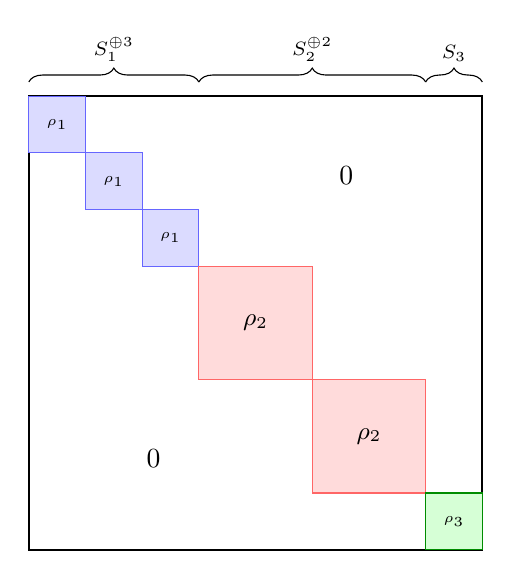
\begin{tikzpicture}[scale=0.72]
	\draw[thick] (0,0) rectangle (8,8);
	% S1 isotypic, three copies of a 1x1
	\draw[fill=blue!14, draw=blue!60] (0,7) rectangle (1,8);
	\draw[fill=blue!14, draw=blue!60] (1,6) rectangle (2,7);
	\draw[fill=blue!14, draw=blue!60] (2,5) rectangle (3,6);
	% S2 isotypic, two copies of a 2x2
	\draw[fill=red!14, draw=red!60] (3,3) rectangle (5,5);
	\draw[fill=red!14, draw=red!60] (5,1) rectangle (7,3);
	% S3 isotypic
	\draw[fill=green!16, draw=green!55!black] (7,0) rectangle (8,1);
	\node at (0.5,7.5) {\tiny $\rho_1$};
	\node at (1.5,6.5) {\tiny $\rho_1$};
	\node at (2.5,5.5) {\tiny $\rho_1$};
	\node at (4,4) {\small $\rho_2$};
	\node at (6,2) {\small $\rho_2$};
	\node at (7.5,0.5) {\tiny $\rho_3$};
	\node at (5.6,6.6) {$0$};
	\node at (2.2,1.6) {$0$};
	% braces
	\draw[decorate, decoration={brace, amplitude=5pt}] (0,8.25) -- (3,8.25) node[midway, above=4pt] {\scriptsize $S_1^{\oplus 3}$};
	\draw[decorate, decoration={brace, amplitude=5pt}] (3,8.25) -- (7,8.25) node[midway, above=4pt] {\scriptsize $S_2^{\oplus 2}$};
	\draw[decorate, decoration={brace, amplitude=5pt}] (7,8.25) -- (8,8.25) node[midway, above=4pt] {\scriptsize $S_3$};
\end{tikzpicture}
\end{center}
\vspace{0.5em}

We can also read off, from Schur's lemma, exactly how big the space of self-maps is.

\begin{proposition}
	If $V \cong \bigoplus_S S^{\oplus n_S}$ then $\dim \End_G(V) = \sum_S n_S^2$. In particular $V$ is irreducible if and only if $\dim\End_G(V) = 1$.
\end{proposition}
\begin{proof}
	Expanding $\Hom_G(\bigoplus_S S^{\oplus n_S}, \bigoplus_T T^{\oplus n_T})$ into a double sum and applying Schur gives $\sum_S n_S^2$. If this is $1$ then exactly one $n_S$ is $1$ and the rest vanish, so $V \cong S$ is irreducible; the converse is Schur.
\end{proof}

This is a genuinely useful irreducibility criterion, and it is the shadow of the character-theoretic criterion $\ip{\chi}{\chi} = 1$ that we will meet shortly.

Finally, let us record what Schur says about the regular representation, since it foreshadows the main counting theorem.

\begin{proposition}
	Let $V$ be a representation of the finite group $G$ and let $S$ be irreducible. Then the multiplicity of $S$ in the regular representation $\C G$ is $\dim S$.
\end{proposition}
\begin{proof}
	By the multiplicity formula it suffices to show $\dim \Hom_G(\C G, S) = \dim S$. Now a $\C G$-module homomorphism $\varphi : \C G \to S$ is determined by $\varphi(e) \in S$, since $\varphi(g) = \varphi(g \cdot e) = g\varphi(e)$ and the $g$ span $\C G$; and conversely any choice of $\varphi(e) = s \in S$ gives a well defined homomorphism $\sum \lambda_g g \mapsto \sum \lambda_g \, g s$. So $\Hom_G(\C G, S) \cong S$ as vector spaces.
\end{proof}

\begin{corollary}
	If $S_1, \dots, S_r$ are the distinct irreducible complex representations of $G$, with $d_i = \dim S_i$, then
	$$\C G \cong \bigoplus_{i=1}^r S_i^{\oplus d_i}, \qquad \text{and hence} \qquad |G| = \sum_{i=1}^r d_i^2.$$
\end{corollary}
\begin{proof}
	The first statement is the proposition, once we know that every irreducible appears -- which it does, with multiplicity $d_i \geq 1$. Comparing dimensions gives $|G| = \sum_i d_i \cdot \dim S_i = \sum d_i^2$.
\end{proof}

We have implicitly used that there are only finitely many irreducibles; this follows since each appears in $\C G$, which is finite dimensional. This identity $|G| = \sum d_i^2$ is one of the two great numerical constraints on the character table -- the other being that $r$ is the number of conjugacy classes. It is remarkably effective: for example, if $|G| = 8$ then the only possibilities for the multiset $\{d_i\}$ with all $d_i \geq 1$ and at least one $d_i = 1$ (the trivial representation) are $\{1,1,1,1,1,1,1,1\}$ and $\{1,1,1,1,2\}$.

\section{Character Theory}

We now come to the heart of the course. The idea is almost absurdly reductive: given a representation $\rho : G \to \GL(V)$, throw away everything about $\rho(g)$ except its trace. What is left is a function $G \to \C$, and it turns out to remember the representation completely.

Why should the trace be the right thing to keep? Because it is the simplest invariant of a linear map which does not depend on a choice of basis, and isomorphic representations differ exactly by a choice of basis.

\subsection{Characters}

\begin{definition}[Character]
	Let $(\rho, V)$ be a representation of $G$ over $\C$. The \vocab{character} of $\rho$ is the function
	$$\chi_V = \chi_\rho : G \to \C, \qquad \chi_\rho(g) = \tr \rho(g),$$
	where the trace is that of the matrix of $\rho(g)$ in any basis. The \vocab{degree} of $\chi$ is $\chi(e) = \dim V$.
\end{definition}

\begin{definition}[Irreducible and linear characters]
	A character is \vocab{irreducible} if it is the character of an irreducible representation. It is \vocab{linear} if it has degree $1$; equivalently, if $\rho : G \to \C^\times$ is a homomorphism.
\end{definition}

Since we will spend the rest of the course computing with characters, we had better establish their basic properties. Every single one of the following is used constantly.

\begin{proposition}[Basic properties]
	Let $(\rho, V)$ be a complex representation of a finite group $G$, with character $\chi$. Then:
	\begin{enumerate}[label=(\roman*)]
		\item $\chi(e) = \dim V$.
		\item $\chi$ is a \vocab{class function}: $\chi(hgh^{-1}) = \chi(g)$ for all $g,h \in G$.
		\item Isomorphic representations have equal characters.
		\item For each $g$, $\chi(g)$ is a sum of $\dim V$ roots of unity; specifically, if $g$ has order $n$ then $\chi(g)$ is a sum of $n$-th roots of unity.
		\item $\chi(g^{-1}) = \overline{\chi(g)}$.
		\item $|\chi(g)| \leq \chi(e)$, with equality if and only if $\rho(g)$ is a scalar.
		\item $\chi(g) = \chi(e)$ if and only if $g \in \kernel\rho$.
	\end{enumerate}
\end{proposition}
\begin{proof}
	(i) $\rho(e) = \id_V$, whose trace is $\dim V$.

	(ii) $\tr(\rho(h)\rho(g)\rho(h)^{-1}) = \tr \rho(g)$, since trace is invariant under conjugation.

	(iii) If $\varphi$ is an isomorphism with $\rho'(g) = \varphi\rho(g)\varphi^{-1}$, take traces.

	(iv) The element $\rho(g)$ satisfies $\rho(g)^n = \id$, so it is diagonalisable with eigenvalues $\lambda_1, \dots, \lambda_d$ ($d = \dim V$) satisfying $\lambda_i^n = 1$, and $\chi(g) = \sum \lambda_i$.

	(v) With notation as in (iv), $\rho(g^{-1}) = \rho(g)^{-1}$ has eigenvalues $\lambda_i^{-1} = \overline{\lambda_i}$ (as $|\lambda_i| = 1$). So $\chi(g^{-1}) = \sum \overline{\lambda_i} = \overline{\chi(g)}$.

	(vi) By the triangle inequality $|\chi(g)| = |\sum\lambda_i| \leq \sum|\lambda_i| = d = \chi(e)$. Equality in the triangle inequality for complex numbers of modulus $1$ forces all $\lambda_i$ to be equal, say to $\lambda$; and then $\rho(g) = \lambda\id_V$ since $\rho(g)$ is diagonalisable.

	(vii) If $g \in \kernel\rho$ then $\rho(g) = \id$ so $\chi(g) = d$. Conversely if $\chi(g) = d$ then equality holds in (vi), so $\rho(g) = \lambda \id$ with $d\lambda = d$, giving $\lambda = 1$.
\end{proof}

Property (vii) is the reason non-faithful representations are useful: characters detect kernels, so from the character table we can read off all the normal subgroups of $G$. We will come back to this.

\begin{proposition}
	If $V, W$ are representations of $G$ then $\chi_{V \oplus W} = \chi_V + \chi_W$.
\end{proposition}
\begin{proof}
	In a basis adapted to the decomposition, $\rho(g)$ is block diagonal with blocks $\rho_V(g)$ and $\rho_W(g)$, and the trace of a block diagonal matrix is the sum of the traces of its blocks.
\end{proof}

So characters of representations are exactly the nonnegative integer combinations of irreducible characters. Such things are sometimes called \emph{proper} characters, or just characters; $\Z$-linear combinations of irreducible characters are called \vocab{virtual characters} or \vocab{generalised characters}.

\begin{example}[The regular character]
	Let $\pi_{\text{reg}}$ be the character of the regular representation $\C G$. In the basis $\{e_g\}$, the matrix of $\rho(h)$ is the permutation matrix of left multiplication by $h$, and its trace counts the $g$ with $hg = g$. So
	$$\pi_{\text{reg}}(g) = \begin{cases} |G| & g = e, \\ 0 & g \neq e.\end{cases}$$
\end{example}

\begin{example}[Permutation characters]
	More generally, if $G$ acts on a finite set $X$ and $\C X$ is the associated permutation representation, then the matrix of $\rho(g)$ has $(x,x)$ entry $1$ exactly when $g\cdot x = x$, and so
	$$\pi_X(g) = |\operatorname{fix}_X(g)| = |\{x \in X: g\cdot x = x\}|.$$
	This is an extremely convenient supply of characters, since counting fixed points is easy.
\end{example}

\begin{example}
	Take $G = S_4$ acting on $X = \{1,2,3,4\}$. Then $\pi_X(e) = 4$, $\pi_X((1\,2)) = 2$, $\pi_X((1\,2)(3\,4)) = 0$, $\pi_X((1\,2\,3)) = 1$ and $\pi_X((1\,2\,3\,4)) = 0$.
\end{example}

\subsection{Class Functions and the Inner Product}

\begin{definition}[Class function]
	A \vocab{class function} on $G$ is a function $f : G \to \C$ which is constant on conjugacy classes. The set of class functions is written $\mathcal{C}(G)$.
\end{definition}

$\mathcal{C}(G)$ is a $\C$-vector space under pointwise operations, and it has an obvious basis: the indicator functions $\delta_{\mathcal{K}}$ of the conjugacy classes $\mathcal{K}$. So
$$\dim_\C \mathcal{C}(G) = \#\{\text{conjugacy classes of } G\} =: r.$$
Characters are class functions, so all the characters of $G$ live in this one $r$-dimensional space -- already a strong constraint, and the source of everything that follows.

We make $\mathcal{C}(G)$ into an inner product space in the natural way.

\begin{definition}[Inner product of class functions]
	For $f, f' \in \mathcal{C}(G)$ define
	$$\ip{f}{f'} = \frac{1}{|G|}\sum_{g \in G} \overline{f(g)}\, f'(g).$$
\end{definition}

This is a Hermitian inner product (linear in the second slot, conjugate-linear in the first, and positive definite since $\ip ff = \frac1{|G|}\sum|f(g)|^2$). If we group the sum by conjugacy classes with representatives $g_1, \dots, g_r$, it becomes
$$\ip{f}{f'} = \sum_{j=1}^r \frac{|\ccl_G(g_j)|}{|G|}\overline{f(g_j)}f'(g_j) = \sum_{j=1}^r \frac{\overline{f(g_j)}f'(g_j)}{|\Cent_G(g_j)|},$$
using $|\ccl_G(g)| \cdot |\Cent_G(g)| = |G|$. This is the form we use in practice.

\begin{remark}
	If $f, f'$ are \emph{characters}, then $\overline{f(g)} = f(g^{-1})$, so
	$$\ip{f}{f'} = \frac{1}{|G|}\sum_{g\in G} f(g^{-1})f'(g),$$
	which is visibly symmetric in $f$ and $f'$. So on characters the inner product is symmetric and we need not fret about which slot is conjugated.
\end{remark}

\subsection{The Orthogonality Relations}

We now prove the central theorem of the course. The strategy is to identify $\ip{\chi_V}{\chi_W}$ with $\dim \Hom_G(V,W)$, and then apply Schur's lemma. Two lemmas do the work.

\begin{lemma}[Fixed points]
	Let $V$ be a representation of $G$ with character $\chi$, and let
	$$V^G = \{ v \in V \mid gv = v \text{ for all } g \in G\}$$
	be the subspace of $G$-invariant vectors. Then
	$$\dim V^G = \frac{1}{|G|}\sum_{g\in G}\chi(g).$$
\end{lemma}
\begin{proof}
	Consider
	$$\pi = \frac1{|G|}\sum_{g \in G}\rho(g) \; \in \; \End(V).$$
	First, $\image \pi \subseteq V^G$: for $h \in G$,
	$$\rho(h)\pi = \frac1{|G|}\sum_{g}\rho(hg) = \frac1{|G|}\sum_{g'}\rho(g') = \pi,$$
	reindexing. Second, $\pi|_{V^G} = \id$: if $v \in V^G$ then every $\rho(g)v = v$, and we average $|G|$ copies of $v$.

	Together these give $\pi^2 = \pi$, so $\pi$ is a projection with image $V^G$. A projection is diagonalisable with eigenvalues $0$ and $1$, and the multiplicity of the eigenvalue $1$ is $\dim \image \pi$. Hence
	$$\dim V^G = \tr \pi = \frac1{|G|}\sum_g \tr\rho(g) = \frac1{|G|}\sum_g \chi(g). \qedhere$$
\end{proof}

\begin{lemma}[The Hom representation]
	Let $V, W$ be representations of $G$. Then $\Hom_\C(V,W)$ becomes a representation of $G$ via
	$$(g\cdot \varphi)(v) = g\,\varphi(g^{-1}v),$$
	and
	\begin{enumerate}[label=(\roman*)]
		\item $\Hom_\C(V,W)^G = \Hom_G(V,W)$;
		\item its character is $\chi_{\Hom(V,W)}(g) = \overline{\chi_V(g)}\,\chi_W(g)$.
	\end{enumerate}
\end{lemma}
\begin{proof}
	That this is a representation is a direct check: $(e\cdot\varphi) = \varphi$, and
	$$(g\cdot(h\cdot\varphi))(v) = g\,(h\cdot\varphi)(g^{-1}v) = gh\,\varphi(h^{-1}g^{-1}v) = ((gh)\cdot\varphi)(v).$$

	(i) We have $g\cdot\varphi = \varphi$ for all $g$ if and only if $g\varphi(g^{-1}v) = \varphi(v)$ for all $g, v$, if and only if $\varphi(g^{-1}v) = g^{-1}\varphi(v)$ for all $g,v$, which is exactly $G$-linearity.

	(ii) Fix $g \in G$. Both $\rho_V(g)$ and $\rho_W(g)$ are diagonalisable, so choose eigenbases $v_1, \dots, v_n$ of $V$ and $w_1, \dots, w_m$ of $W$ with $gv_i = \lambda_i v_i$ and $gw_j = \mu_j w_j$, where all $\lambda_i, \mu_j$ are roots of unity. Let $\varphi_{ij} \in \Hom(V,W)$ be defined by $\varphi_{ij}(v_k) = \delta_{ik}w_j$; these $nm$ maps form a basis. Then
	$$(g\cdot\varphi_{ij})(v_k) = g\,\varphi_{ij}(\lambda_k^{-1}v_k) = \lambda_k^{-1}\delta_{ik}\, gw_j = \lambda_i^{-1}\mu_j\,\varphi_{ij}(v_k),$$
	so $\varphi_{ij}$ is an eigenvector with eigenvalue $\lambda_i^{-1}\mu_j = \overline{\lambda_i}\mu_j$. Summing,
	$$\chi_{\Hom(V,W)}(g) = \sum_{i,j}\overline{\lambda_i}\mu_j = \Big(\sum_i \overline{\lambda_i}\Big)\Big(\sum_j \mu_j\Big) = \overline{\chi_V(g)}\chi_W(g). \qedhere$$
\end{proof}

Putting these together gives the key identity.

\begin{theorem}
	For any representations $V, W$ of the finite group $G$,
	$$\ip{\chi_V}{\chi_W} = \dim_\C \Hom_G(V,W).$$
\end{theorem}
\begin{proof}
	Apply the fixed point lemma to the representation $\Hom_\C(V,W)$:
	$$\dim \Hom_G(V,W) = \dim \Hom_\C(V,W)^G = \frac1{|G|}\sum_{g}\chi_{\Hom(V,W)}(g) = \frac1{|G|}\sum_g \overline{\chi_V(g)}\chi_W(g),$$
	which is $\ip{\chi_V}{\chi_W}$.
\end{proof}

\begin{theorem}[Row orthogonality]
	Let $\chi_1, \dots, \chi_r$ be the characters of the distinct (i.e. pairwise non-isomorphic) irreducible complex representations $S_1, \dots, S_r$ of the finite group $G$. Then
	$$\ip{\chi_i}{\chi_j} = \delta_{ij}.$$
	That is, the irreducible characters are orthonormal in $\mathcal{C}(G)$.
\end{theorem}
\begin{proof}
	Immediate from the previous theorem and Schur's lemma, which says $\dim \Hom_G(S_i, S_j)$ is $1$ if $i=j$ and $0$ otherwise.
\end{proof}

That is the whole proof, and it is worth appreciating how little it needed: averaging (Maschke's idea), a trace computation, and Schur. Written out in coordinates the statement is
$$\frac1{|G|}\sum_{g \in G}\overline{\chi_i(g)}\chi_j(g) = \sum_{k=1}^r \frac{\overline{\chi_i(g_k)}\chi_j(g_k)}{|\Cent_G(g_k)|} = \delta_{ij},$$
a system of $\binom{r+1}{2}$ equations relating the entries of the character table. In practice these equations are so restrictive that they often determine the entire table.

\begin{remark}
	There is a more computational proof, which is the one Frobenius gave. One takes an arbitrary linear map $\psi : S_i \to S_j$, averages it to $\tilde\psi = \frac1{|G|}\sum_g \rho_j(g)\psi\rho_i(g)^{-1}$, applies Schur to $\tilde\psi$, and then reads off matrix entries. It gives the same relations, with more index-pushing and less insight; the reader may enjoy carrying it out.
\end{remark}

\subsection{Consequences of Orthogonality}

The corollaries come thick and fast. Throughout, $\chi_1, \dots, \chi_r$ are the irreducible characters of $G$.

\begin{corollary}
	The irreducible characters are linearly independent in $\mathcal{C}(G)$. In particular $r \leq \#\{\text{conjugacy classes}\}$, so $G$ has only finitely many irreducible representations up to isomorphism.
\end{corollary}
\begin{proof}
	Orthonormal sets are linearly independent, and $\dim\mathcal{C}(G)$ is the number of conjugacy classes.
\end{proof}

\begin{corollary}[Decomposition]
	Let $V$ be a representation with character $\chi$, and write $V \cong \bigoplus_i S_i^{\oplus n_i}$. Then
	$$\chi = \sum_i n_i \chi_i, \qquad n_i = \ip{\chi_i}{\chi} = \ip{\chi}{\chi_i}.$$
\end{corollary}
\begin{proof}
	Characters add over direct sums, giving the first formula; then take the inner product with $\chi_i$ and use orthonormality. (The two expressions for $n_i$ agree because $n_i$ is real.)
\end{proof}

\begin{corollary}[Characters determine representations]
	Two complex representations of a finite group are isomorphic if and only if they have the same character.
\end{corollary}
\begin{proof}
	One direction we knew. Conversely, if $\chi_V = \chi_W$ then the multiplicities $n_i = \ip{\chi_i}{\chi_V} = \ip{\chi_i}{\chi_W}$ agree for every $i$, and a representation is determined up to isomorphism by its multiplicities.
\end{proof}

This is a genuinely surprising statement. A representation of $G$ of degree $d$ is a huge amount of data -- $|G|$ matrices of size $d\times d$ -- and it is all encoded in $r$ complex numbers.

\begin{corollary}[Irreducibility criterion]
	A representation $V$ with character $\chi$ is irreducible if and only if $\ip\chi\chi = 1$.
\end{corollary}
\begin{proof}
	Writing $\chi = \sum n_i\chi_i$, orthonormality gives $\ip\chi\chi = \sum_i n_i^2$. Since the $n_i$ are nonnegative integers, this equals $1$ if and only if exactly one $n_i$ is $1$ and the rest are $0$, i.e. $V \cong S_i$ is irreducible.
\end{proof}

This is the workhorse of the whole subject: to check irreducibility we compute a single number.

\begin{example}[The standard representation of $S_n$ is irreducible]
	Let $\pi$ be the permutation character of $S_n$ on $\{1,\dots,n\}$, so $\pi(\sigma) = |\operatorname{fix}(\sigma)|$. By Burnside's lemma (orbit counting),
	$$\ip{\pi}{\mathbf{1}} = \frac1{|G|}\sum_\sigma |\operatorname{fix}(\sigma)| = \#\{\text{orbits}\} = 1,$$
	and
	$$\ip\pi\pi = \frac1{|G|}\sum_\sigma|\operatorname{fix}(\sigma)|^2 = \#\{\text{orbits of } S_n \text{ on } \{1,\dots,n\}^2\} = 2$$
	for $n \geq 2$ (the diagonal, and its complement). Since $\pi = \mathbf 1 + \chi$ where $\chi$ is the character of the standard representation, we get
	$$2 = \ip\pi\pi = \ip{\mathbf1 + \chi}{\mathbf 1 + \chi} = 1 + 2\ip{\mathbf1}\chi + \ip\chi\chi = 1 + \ip\chi\chi,$$
	using $\ip{\mathbf1}{\chi} = \ip{\mathbf1}{\pi} - 1 = 0$. So $\ip\chi\chi = 1$ and the standard representation is irreducible, of degree $n-1$.
\end{example}

\begin{remark}
	The computation above works verbatim for any \vocab{$2$-transitive} action of a group $G$ on a set $X$: `$2$-transitive' means $G$ acts transitively on ordered pairs of distinct elements, which is exactly the statement that there are two orbits on $X \times X$. So for any $2$-transitive action, $\pi_X - \mathbf 1$ is an irreducible character of degree $|X| - 1$. This gives irreducible characters for free for $S_n$, $A_n$ ($n\geq 4$), $\PGL_2(\F_q)$ acting on the projective line, and many others.
\end{remark}

\subsection{Counting the Irreducibles}

We know $r \leq \#\{\text{conjugacy classes}\}$. We now show equality, which is the second great numerical constraint.

\begin{theorem}
	The irreducible characters $\chi_1, \dots, \chi_r$ form an orthonormal \emph{basis} of $\mathcal{C}(G)$. Consequently, the number of irreducible complex representations of $G$ equals the number of conjugacy classes of $G$.
\end{theorem}
\begin{proof}
	We already know they are orthonormal, so it suffices to show that the only class function orthogonal to all of them is $0$.

	So let $f \in \mathcal{C}(G)$ with $\ip{f}{\chi_i} = 0$ for all $i$. For any representation $(\rho, V)$ define
	$$\varphi_f = \sum_{g\in G}\overline{f(g)}\,\rho(g) \; \in \; \End(V).$$
	We claim $\varphi_f$ is $G$-linear. Indeed, for $h \in G$,
	$$\varphi_f\,\rho(h) = \sum_g \overline{f(g)}\rho(gh) = \sum_k \overline{f(kh^{-1})}\rho(k), \qquad \rho(h)\,\varphi_f = \sum_g \overline{f(g)}\rho(hg) = \sum_k\overline{f(h^{-1}k)}\rho(k),$$
	substituting $k = gh$ and $k = hg$ respectively. But $f$ is a class function, so
	$$f(kh^{-1}) = f\big(h^{-1}(kh^{-1})h\big) = f(h^{-1}k),$$
	and the two expressions agree.

	Now take $V = S_i$ irreducible, of degree $d_i$. By Schur, $\varphi_f = \lambda\id$ for some $\lambda \in \C$, and taking traces,
	$$d_i \lambda = \tr\varphi_f = \sum_g \overline{f(g)}\chi_i(g) = |G|\ip{f}{\chi_i} = 0,$$
	so $\lambda = 0$ and $\varphi_f = 0$ on every irreducible representation. By complete reducibility, $\varphi_f = 0$ on \emph{every} representation of $G$.

	Apply this to the regular representation $V = \C G$, and evaluate at the basis vector $e$:
	$$0 = \varphi_f(e) = \sum_{g\in G}\overline{f(g)}\, g.$$
	The elements $g \in G$ are a basis of $\C G$, so $\overline{f(g)} = 0$ for every $g$, i.e. $f = 0$.
\end{proof}

\begin{corollary}
	A finite group $G$ is abelian if and only if all its irreducible complex representations have degree $1$.
\end{corollary}
\begin{proof}
	We proved `only if' earlier. Conversely, if all $d_i = 1$ then $|G| = \sum_i d_i^2 = r$, so $G$ has $|G|$ conjugacy classes, meaning every class is a singleton, meaning every element is central.
\end{proof}

\subsection{The Character Table}

We can now assemble everything into the object which gives the subject its computational character.

\begin{definition}[Character table]
	Let $G$ have conjugacy classes with representatives $g_1 = e, g_2, \dots, g_r$ and irreducible characters $\chi_1 = \mathbf 1, \chi_2, \dots, \chi_r$. The \vocab{character table} of $G$ is the $r \times r$ matrix
	$$X = \big(\chi_i(g_j)\big)_{1\leq i,j\leq r}.$$
	By convention we list the trivial character first and the identity class first, and we record the class sizes $|\ccl_G(g_j)|$ (or the centraliser orders) alongside.
\end{definition}

It is a square matrix -- that is the content of the counting theorem -- and it satisfies two orthogonality relations, one for rows and one for columns. Schematically:

\begin{center}
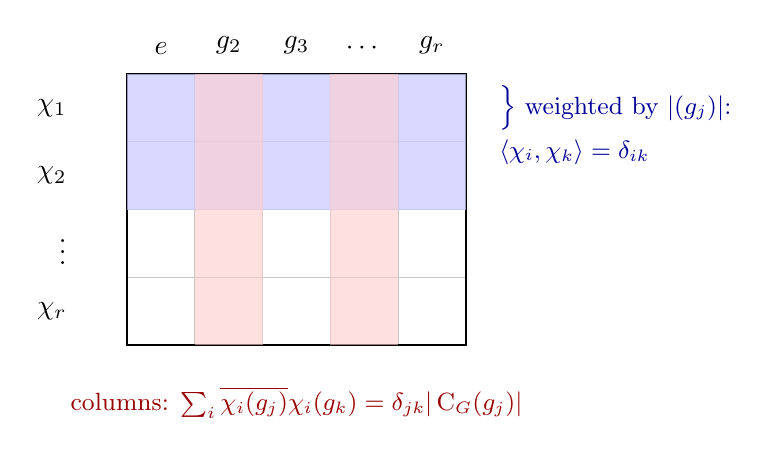
\begin{tikzpicture}[scale=0.86]
	% grid
	\foreach \i in {0,...,4} { \draw[gray!45] (0,\i) -- (5,\i); }
	\foreach \j in {0,...,5} { \draw[gray!45] (\j,0) -- (\j,4); }
	\draw[thick] (0,0) rectangle (5,4);
	% labels
	\node[left] at (-0.75,3.5) {$\chi_1$};
	\node[left] at (-0.75,2.5) {$\chi_2$};
	\node[left] at (-0.75,1.5) {$\vdots$};
	\node[left] at (-0.75,0.5) {$\chi_r$};
	\node[above] at (0.5,4.15) {$e$};
	\node[above] at (1.5,4.15) {$g_2$};
	\node[above] at (2.5,4.15) {$g_3$};
	\node[above] at (3.5,4.15) {$\cdots$};
	\node[above] at (4.5,4.15) {$g_r$};
	% highlight two rows
	\fill[blue!20, opacity=0.75] (0,3) rectangle (5,4);
	\fill[blue!20, opacity=0.75] (0,2) rectangle (5,3);
	% highlight two columns
	\fill[red!20, opacity=0.6] (1,0) rectangle (2,4);
	\fill[red!20, opacity=0.6] (3,0) rectangle (4,4);
	\node[blue!60!black, right] at (5.35,3.5) {\small $\Big\}$ weighted by $|\ccl(g_j)|$:};
	\node[blue!60!black, right] at (5.35,2.85) {\small $\ip{\chi_i}{\chi_k} = \delta_{ik}$};
	\node[red!60!black] at (2.5,-0.85) {\small columns: $\sum_i \overline{\chi_i(g_j)}\chi_i(g_k) = \delta_{jk}|\Cent_G(g_j)|$};
\end{tikzpicture}
\end{center}
\vspace{0.3em}

Let us prove the column relation. It is a formal consequence of the row relation, by a small piece of matrix algebra.

\begin{theorem}[Column orthogonality]
	With notation as above, for any $1 \leq j, k \leq r$,
	$$\sum_{i=1}^r \overline{\chi_i(g_j)}\,\chi_i(g_k) = \delta_{jk}\,|\Cent_G(g_j)|.$$
	In particular, taking $j = k = 1$ recovers $\sum_i d_i^2 = |G|$.
\end{theorem}
\begin{proof}
	Let $D$ be the diagonal matrix with entries $D_{jj} = |\ccl_G(g_j)|/|G| = 1/|\Cent_G(g_j)|$. Row orthogonality says
	$$\delta_{ik} = \ip{\chi_k}{\chi_i} = \sum_j \frac{\overline{\chi_k(g_j)}\chi_i(g_j)}{|\Cent_G(g_j)|} = \big(X D \overline{X}^{\,T}\big)_{ik},$$
	so $X D \overline X^{\,T} = I$. Thus the square matrix $X$ is invertible with $X^{-1} = D\overline X^{\,T}$, and therefore $X^{-1}X = I$ as well:
	$$I = D\overline X^{\,T} X, \qquad \text{i.e.}\qquad \delta_{jk} = \frac{1}{|\Cent_G(g_j)|}\sum_i \overline{\chi_i(g_j)}\chi_i(g_k),$$
	which rearranges to the claim.
\end{proof}

\begin{corollary}
	Taking $j = k$, for every $g \in G$ we have $\sum_i |\chi_i(g)|^2 = |\Cent_G(g)|$.
\end{corollary}

Column orthogonality is enormously useful in practice: it lets us fill in a missing row or column of a character table once the rest is known, and it provides an independent check on every table we compute. Whenever the reader writes down a character table, they should verify:
\begin{enumerate}[label=(\roman*)]
	\item the table is square, with $r$ = number of conjugacy classes;
	\item $\sum_i d_i^2 = |G|$;
	\item each row has $\ip{\chi_i}{\chi_i} = 1$ and distinct rows are orthogonal;
	\item each column $j$ satisfies $\sum_i|\chi_i(g_j)|^2 = |\Cent_G(g_j)| = |G|/|\ccl(g_j)|$.
\end{enumerate}
All of the tables in these notes have been checked against all four.

\begin{corollary}
	Let $g \in G$ with $g \neq e$. Then $\sum_i d_i \chi_i(g) = 0$.
\end{corollary}
\begin{proof}
	This is column orthogonality applied to the columns of $e$ and of $g$, using $\chi_i(e) = d_i$; alternatively, it says $\pi_{\text{reg}}(g) = 0$, which we computed directly.
\end{proof}

\subsection{First Character Tables}

Let us put the machinery to work.

\begin{example}[Cyclic groups]
	Let $G = C_m = \gen{g}$. Every element is its own conjugacy class, so $r = m$, and all irreducibles have degree $1$ since $G$ is abelian. Indeed $\sum_{i=1}^m d_i^2 = m$ forces every $d_i = 1$. The characters are $\chi_j(g^k) = \omega^{jk}$ with $\omega = e^{2\pi i/m}$. For $m = 4$, with $i = \sqrt{-1}$:
	\begin{center}
	\renewcommand{\arraystretch}{1.25}
	\setlength{\tabcolsep}{9pt}
	\begin{tabular}{c|cccc}
	\toprule
	 & $e$ & $g$ & $g^2$ & $g^3$\\
	\midrule
	$\chi_0$ & $1$ & $1$ & $1$ & $1$\\
	$\chi_1$ & $1$ & $i$ & $-1$ & $-i$\\
	$\chi_2$ & $1$ & $-1$ & $1$ & $-1$\\
	$\chi_3$ & $1$ & $-i$ & $-1$ & $i$\\
	\bottomrule
	\end{tabular}
	\end{center}
	Every centraliser is all of $G$, of order $4$, and indeed every column has $\sum_i|\chi_i(g^k)|^2 = 4$. Rows are orthogonal because $\sum_{k=0}^3 \omega^{(j - j')k} = 0$ for $j \neq j'$ -- the character table of a cyclic group is (a scalar multiple of) the discrete Fourier transform matrix.
\end{example}

\begin{example}[$S_3$]
	The group $S_3$ has order $6$ and three conjugacy classes, with representatives $e$, $(1\,2)$ and $(1\,2\,3)$, of sizes $1, 3, 2$. So there are three irreducible characters with $d_1^2 + d_2^2 + d_3^2 = 6$; since $d_i \geq 1$ and at least one $d_i = 1$, the only solution is $\{1,1,2\}$.

	We know two of the degree-$1$ characters already: the trivial character and the sign character. The degree-$2$ character is that of the standard representation, which we showed is irreducible; its character is $\pi - \mathbf 1$ where $\pi$ is the permutation character $\pi = (3,1,0)$. So $\chi_3 = (2, 0, -1)$. Alternatively, column orthogonality determines the last row up to a scalar of modulus one.
	\begin{center}
	\renewcommand{\arraystretch}{1.25}
	\setlength{\tabcolsep}{10pt}
	\begin{tabular}{c|ccc}
	\toprule
	class size & $1$ & $3$ & $2$\\
	 & $e$ & $(1\,2)$ & $(1\,2\,3)$\\
	\midrule
	$\mathbf 1$ & $1$ & $1$ & $1$\\
	$\sign$ & $1$ & $-1$ & $1$\\
	$\chi_3$ & $2$ & $0$ & $-1$\\
	\bottomrule
	\end{tabular}
	\end{center}
	Let us verify. Degrees: $1 + 1 + 4 = 6 = |S_3|$. Rows: $\ip{\chi_3}{\chi_3} = \frac16(1\cdot 4 + 3\cdot 0 + 2\cdot 1) = \frac{6}{6} = 1$; $\ip{\mathbf1}{\chi_3} = \frac16(2 + 0 - 2) = 0$; $\ip{\mathbf1}{\sign} = \frac16(1 - 3 + 2) = 0$; $\ip{\sign}{\chi_3} = \frac16(2 - 0 - 2) = 0$. Columns: $1 + 1 + 4 = 6 = |\Cent(e)|$; $1 + 1 + 0 = 2 = |\Cent((1\,2))| = 6/3$; $1+1+1 = 3 = |\Cent((1\,2\,3))| = 6/2$. Everything checks out.
\end{example}

\begin{example}[Recovering a row]
	Suppose we know that a group $G$ of order $12$ has four conjugacy classes of sizes $1,3,4,4$ and that three of its irreducible characters are $(1,1,1,1)$, $(1,1,\omega,\omega^2)$, $(1,1,\omega^2,\omega)$ where $\omega = e^{2\pi i/3}$. Then the degrees satisfy $1+1+1+d_4^2 = 12$, so $d_4 = 3$; and column orthogonality against the first column gives, for the class of size $3$,
	$$1\cdot 1 + 1\cdot 1 + 1\cdot 1 + 3\,\chi_4(g_2) = 0 \implies \chi_4(g_2) = -1,$$
	and similarly $1 + \omega^2 + \omega + 3\chi_4(g_3) = 0$ gives $\chi_4(g_3) = 0$, and likewise $\chi_4(g_4) = 0$. The group, of course, is $A_4$; we will meet it again.
\end{example}

\section{Permutation Representations and Normal Subgroups}

Before building more representations by algebraic means, let us extract everything we can from the ones we get for free -- those coming from actions on sets -- and see how the character table detects the normal subgroup structure of $G$.

\subsection{Permutation Characters}

Recall that an action of $G$ on a finite set $X$ gives the permutation representation $\C X$, with character $\pi_X(g) = |\operatorname{fix}_X(g)|$.

\begin{proposition}
	Let $G$ act on the finite set $X$, with permutation character $\pi_X$.
	\begin{enumerate}[label=(\roman*)]
		\item $\ip{\pi_X}{\mathbf 1}$ is the number of orbits of $G$ on $X$.
		\item $\ip{\pi_X}{\pi_X}$ is the number of orbits of $G$ on $X\times X$.
		\item If $|X| \geq 2$ and $G$ is transitive on $X$, then $\pi_X - \mathbf 1$ is a character of degree $|X|-1$; it is irreducible if and only if $G$ is $2$-transitive on $X$.
	\end{enumerate}
\end{proposition}
\begin{proof}
	(i) This is Burnside's orbit-counting lemma: $\ip{\pi_X}{\mathbf 1} = \frac1{|G|}\sum_g|\operatorname{fix}(g)|$, which is the number of orbits.

	(ii) The permutation character of the action on $X \times X$ is $\pi_{X\times X}(g) = |\operatorname{fix}_{X\times X}(g)| = |\operatorname{fix}_X(g)|^2 = \pi_X(g)^2$. Since $\pi_X$ is real valued, $\ip{\pi_X}{\pi_X} = \ip{\pi_{X\times X}}{\mathbf 1}$, and we apply (i).

	(iii) By (i), transitivity gives $\ip{\pi_X}{\mathbf 1} = 1$, so $\mathbf 1$ occurs exactly once in $\pi_X$ and $\chi := \pi_X - \mathbf 1$ is a character (of an actual representation, namely the complement of the fixed line $\gen{\sum_x e_x}$). Then
	$$\ip{\chi}{\chi} = \ip{\pi_X}{\pi_X} - 2\ip{\pi_X}{\mathbf 1} + 1 = \ip{\pi_X}{\pi_X} - 1,$$
	which equals $1$ exactly when $G$ has two orbits on $X\times X$. Since the diagonal is always one orbit, and its complement is a single orbit precisely when $G$ is $2$-transitive, we are done.
\end{proof}

\begin{example}[$S_n$ and $A_n$]
	$S_n$ is $2$-transitive on $\{1,\dots,n\}$ for $n \geq 2$, and $A_n$ is $2$-transitive for $n \geq 4$. So both have an irreducible character of degree $n-1$, the standard character.
\end{example}

\begin{example}[Two-orbit tricks]
	Let $G = S_4$ act on the set $X$ of $\binom42 = 6$ unordered pairs from $\{1,2,3,4\}$. Then $\pi_X = (6, 2, 2, 0, 0)$ on the classes $e, (1\,2), (1\,2)(3\,4), (1\,2\,3), (1\,2\,3\,4)$ -- for instance $(1\,2)$ fixes the pairs $\{1,2\}$ and $\{3,4\}$. Then
	$$\ip{\pi_X}{\pi_X} = \tfrac1{24}\big(36 + 6\cdot 4 + 3\cdot 4 + 0 + 0\big) = \tfrac{72}{24} = 3,$$
	so $\pi_X$ is a sum of three distinct irreducibles (or has some other decomposition with $\sum n_i^2 = 3$, which forces three distinct constituents). Since $\ip{\pi_X}{\mathbf 1} = \frac1{24}(6 + 12 + 6) = 1$, one of them is trivial. This is a good source of characters, and we will use it when building the table of $S_4$.
\end{example}

\subsection{Lifting Characters}

Non-faithful representations of $G$ are really representations of quotients of $G$, and this is a two-way street.

\begin{proposition}[Lifting]
	Let $N \normal G$ with quotient map $q : G \to G/N$. Then
	$$\tilde\rho \longmapsto \rho := \tilde\rho \circ q$$
	is a bijection between representations of $G/N$ and representations of $\rho$ of $G$ with $N \leq \kernel\rho$. It preserves irreducibility, direct sums and isomorphism, and on characters it is $\chi(g) = \tilde\chi(gN)$.
\end{proposition}
\begin{proof}
	If $\tilde\rho : G/N \to \GL(V)$ is a representation then $\rho = \tilde\rho\circ q$ is a composite of homomorphisms, hence a representation of $G$, with $N \leq \kernel \rho$. Conversely if $\rho$ is a representation of $G$ with $N \leq \kernel\rho$ then $\rho$ factors uniquely through $q$ by the universal property of quotient groups. The two constructions are mutually inverse.

	A subspace is $\rho(G)$-invariant if and only if it is $\tilde\rho(G/N)$-invariant, since $\rho(G) = \tilde\rho(G/N)$ as subgroups of $\GL(V)$; so irreducibility is preserved. The character statement is immediate from $\rho(g) = \tilde\rho(gN)$.
\end{proof}

\begin{center}
\begin{tikzpicture}[scale=1]
	\node (G) at (0,1.5) {$G$};
	\node (GL) at (3.4,1.5) {$\GL(V)$};
	\node (Q) at (0,0) {$G/N$};
	\draw[->] (G) -- node[above] {\small $\rho$} (GL);
	\draw[->>] (G) -- node[left] {\small $q$} (Q);
	\draw[->, dashed] (Q) -- node[below right=-2pt] {\small $\tilde\rho$} (GL.south west);
	\node[right] at (4.35,0.6) {\small (exists iff $N \leq \kernel\rho$)};
\end{tikzpicture}
\end{center}

So the character table of $G/N$ sits inside that of $G$: its rows are exactly those $\chi_i$ with $N \leq \kernel\chi_i$, and its columns are the classes of $G/N$, which are the images of the classes of $G$.

\begin{example}[Lifting from $S_3$]
	$S_4$ has the normal subgroup $V_4 = \{e, (1\,2)(3\,4), (1\,3)(2\,4), (1\,4)(2\,3)\}$ with $S_4/V_4 \cong S_3$. Lifting the three irreducible characters of $S_3$ gives three irreducible characters of $S_4$, of degrees $1, 1, 2$: the trivial character, the sign character, and a degree-$2$ character taking the value $2$ on $e$ and on $(1\,2)(3\,4)$, the value $0$ on transpositions and $4$-cycles, and $-1$ on $3$-cycles. This is exactly how we shall build the character table of $S_4$.
\end{example}

More strikingly, the character table sees \emph{all} the normal subgroups.

\begin{proposition}
	Let $\chi$ be a character of $G$. Then $\kernel\chi := \{g \in G : \chi(g) = \chi(e)\}$ is a normal subgroup of $G$, namely the kernel of any representation affording $\chi$.
\end{proposition}
\begin{proof}
	We proved earlier that $\chi(g) = \chi(e)$ if and only if $\rho(g) = \id$.
\end{proof}

\begin{theorem}
	Every normal subgroup of $G$ is an intersection of kernels of irreducible characters. Precisely, if $N \normal G$ then
	$$N = \bigcap \{\kernel\chi_i \; : \; N \leq \kernel \chi_i\}.$$
\end{theorem}
\begin{proof}
	The inclusion $\subseteq$ is clear. For the reverse, note that the irreducible characters $\chi_i$ with $N \leq \kernel\chi_i$ are exactly the lifts of the irreducible characters of $G/N$. Let $g$ lie in the right hand side; then $\tilde\chi(gN) = \tilde\chi(N)$ for every irreducible character $\tilde\chi$ of $G/N$. Since the regular representation of $G/N$ is faithful and decomposes into irreducibles containing every irreducible, the intersection of the kernels of all irreducible representations of any finite group is trivial. Hence $gN = N$, i.e. $g \in N$.
\end{proof}

\begin{corollary}
	A finite group $G$ is simple if and only if for every non-trivial irreducible character $\chi_i$ ($i \neq 1$) and every $g \neq e$, we have $\chi_i(g) \neq \chi_i(e)$.
\end{corollary}
\begin{proof}
	If some $\chi_i \neq \mathbf 1$ has $\chi_i(g) = \chi_i(e)$ with $g \neq e$, then $\kernel\chi_i$ is a normal subgroup containing $g$, and it is proper since $\chi_i$ is not trivial (if $\kernel\chi_i = G$ then $\rho_i$ is trivial so $\chi_i = d_i\mathbf 1$, forcing $d_i=1$ and $\chi_i = \mathbf 1$). Conversely, if $N$ is a proper nontrivial normal subgroup then by the theorem some $\chi_i$ with $i \neq 1$ has $N \leq \kernel \chi_i$, and any $g \in N\setminus\{e\}$ works.
\end{proof}

This is a genuinely practical test, and we will use it to confirm that $A_5$ is simple purely by staring at a $5\times5$ table.

\subsection{Linear Characters and the Derived Subgroup}

The degree-$1$ characters are the easiest to find, and they are exactly accounted for by the abelianisation.

\begin{proposition}
	Let $G' = [G,G]$ be the derived subgroup. The linear characters of $G$ are precisely the lifts of the (linear) characters of the abelian group $G/G'$, and there are exactly $|G/G'|$ of them. They form a group under pointwise multiplication, isomorphic to $G/G'$ when $G/G'$ is written multiplicatively (non-canonically).
\end{proposition}
\begin{proof}
	A homomorphism $\rho : G \to \C^\times$ has abelian image, so $G' \leq \kernel\rho$, so it is a lift from $G/G'$. Conversely all such lifts are linear characters. Since $G/G'$ is abelian, all of its irreducible characters are linear and there are $|G/G'|$ of them.

	Pointwise product of linear characters is a linear character, and the inverse of $\chi$ is $\overline\chi$; so they form a group, which is the character group of the finite abelian group $G/G'$, non-canonically isomorphic to it.
\end{proof}

\begin{example}
	$S_n$ has $S_n' = A_n$ for $n\geq 2$, so $S_n$ has exactly two linear characters: $\mathbf 1$ and $\sign$. $A_5$ is perfect ($A_5' = A_5$), so its only linear character is the trivial one. And $Q_8$ has $Q_8' = \{\pm 1\}$ with quotient $C_2\times C_2$, so $Q_8$ has four linear characters.
\end{example}

\section{New Characters from Old}

We have a good supply of representations coming from group actions, but to fill in a character table we usually need to manufacture more. There are three main constructions -- duals, tensor products, and (later) induction -- and each has a clean effect on characters.

\subsection{Dual Representations}

\begin{definition}[Dual representation]
	Let $(\rho, V)$ be a representation of $G$ and $V^* = \Hom_\C(V,\C)$ its dual space. The \vocab{dual} (or \vocab{contragredient}) representation is
	$$\rho^*(g)(f) = f\circ\rho(g^{-1}), \qquad \text{i.e.} \qquad (g\cdot f)(v) = f(g^{-1}v).$$
\end{definition}

The inverse is essential: without it we would get an antihomomorphism. Note this is the special case $W = \C$ (trivial) of the $\Hom$ representation from the proof of orthogonality.

\begin{proposition}
	$\chi_{V^*}(g) = \chi_V(g^{-1}) = \overline{\chi_V(g)}$.
\end{proposition}
\begin{proof}
	Choose a basis $v_1,\dots,v_n$ of $V$ of eigenvectors for $\rho(g)$, with $gv_i = \lambda_i v_i$, and let $v_1^*,\dots,v_n^*$ be the dual basis. Then $(g\cdot v_i^*)(v_j) = v_i^*(\lambda_j^{-1}v_j) = \lambda_j^{-1}\delta_{ij}$, so $g\cdot v_i^* = \lambda_i^{-1}v_i^*$. Hence $\chi_{V^*}(g) = \sum_i\lambda_i^{-1} = \chi_V(g^{-1})$, which equals $\overline{\chi_V(g)}$ as the $\lambda_i$ are roots of unity.
\end{proof}

\begin{definition}[Self-dual]
	A representation $V$ is \vocab{self-dual} if $V \cong V^*$, equivalently if $\chi_V$ is real valued.
\end{definition}

\begin{proposition}
	If every element of $G$ is conjugate to its inverse (a \vocab{real} group -- for example, any $S_n$, or any $D_{2n}$), then every character of $G$ is real valued and every representation is self-dual.
\end{proposition}
\begin{proof}
	$\overline{\chi(g)} = \chi(g^{-1}) = \chi(g)$ since $\chi$ is a class function and $g^{-1}$ is conjugate to $g$.
\end{proof}

\subsection{Tensor Products}

The tensor product is the construction that makes the set of characters into a ring, and it is by far the most productive way of building new irreducibles from known ones.

Recall from \emph{Groups, Rings and Modules} the tensor product $V \otimes W$ of vector spaces: if $v_1,\dots,v_n$ is a basis of $V$ and $w_1,\dots,w_m$ a basis of $W$, then $V\otimes W$ has basis $\{v_i\otimes w_j\}$, so $\dim(V\otimes W) = \dim V\dim W$, and $\otimes$ is bilinear. Any bilinear map $V \times W \to U$ factors uniquely through a linear map $V \otimes W \to U$.

\begin{definition}[Tensor product of representations]
	If $(\rho, V)$ and $(\rho', W)$ are representations of $G$, define $\rho\otimes\rho'$ on $V\otimes W$ by
	$$g\cdot(v\otimes w) = (gv)\otimes(gw),$$
	extended linearly.
\end{definition}

One should check this is well defined: for fixed $g$, the map $(v,w)\mapsto gv\otimes gw$ is bilinear, so induces a linear map on $V \otimes W$; and $\rho\otimes\rho'(gh) = (\rho\otimes\rho')(g)(\rho\otimes\rho')(h)$ holds on the spanning set of pure tensors.

\begin{proposition}
	$\chi_{V\otimes W}(g) = \chi_V(g)\,\chi_W(g)$.
\end{proposition}
\begin{proof}
	Fix $g$ and choose eigenbases $(v_i)$ for $\rho(g)$ with eigenvalues $\lambda_i$, and $(w_j)$ for $\rho'(g)$ with eigenvalues $\mu_j$. Then $g\cdot(v_i\otimes w_j) = \lambda_i\mu_j\,(v_i\otimes w_j)$, so the $v_i\otimes w_j$ form an eigenbasis and
	$$\chi_{V\otimes W}(g) = \sum_{i,j}\lambda_i\mu_j = \Big(\sum_i\lambda_i\Big)\Big(\sum_j\mu_j\Big) = \chi_V(g)\chi_W(g). \qedhere$$
\end{proof}

\begin{remark}
	Note carefully: this is \emph{not} the same as the representation of $G\times G$ on $V\otimes W$, which we will meet in a moment. Here both factors are acted on by the same $g$; this is sometimes called the `inner' tensor product.
\end{remark}

\begin{corollary}
	$\Hom_\C(V,W) \cong V^*\otimes W$ as representations of $G$.
\end{corollary}
\begin{proof}
	Both have character $\overline{\chi_V}\chi_W$, and characters determine representations. (One can of course write down the isomorphism $f\otimes w\mapsto (v\mapsto f(v)w)$ directly.)
\end{proof}

\begin{proposition}
	If $\chi$ is a character and $\lambda$ is a \emph{linear} character, then $\lambda\chi$ is a character, and $\chi$ is irreducible if and only if $\lambda\chi$ is.
\end{proposition}
\begin{proof}
	$\lambda\chi$ is the character of $L\otimes V$ where $L$ is the one-dimensional space affording $\lambda$. Since $|\lambda(g)| = 1$ for all $g$, we have $\ip{\lambda\chi}{\lambda\chi} = \frac1{|G|}\sum_g|\lambda(g)|^2|\chi(g)|^2 = \ip\chi\chi$, so one is $1$ if and only if the other is.
\end{proof}

This is a cheap and very effective way to produce new irreducibles: tensoring the character table of $S_n$ with $\sign$ permutes its rows.

The tensor product of two irreducibles is usually \emph{not} irreducible, and decomposing it is a basic computation.

\begin{example}
	In $S_3$, with $\chi_3 = (2,0,-1)$ the degree-$2$ character, we have $\chi_3^2 = (4,0,1)$. Then
	$$\ip{\chi_3^2}{\mathbf 1} = \tfrac16(4 + 0 + 2) = 1, \quad \ip{\chi_3^2}{\sign} = \tfrac16(4 - 0 + 2) = 1, \quad \ip{\chi_3^2}{\chi_3} = \tfrac16(8 + 0 - 2) = 1,$$
	so $\chi_3\otimes\chi_3 = \mathbf 1 + \sign + \chi_3$, consistent with degrees $4 = 1+1+2$.
\end{example}

\subsection{Symmetric and Exterior Squares}

The decomposition in the last example was not an accident of $S_3$: for any $V$, the space $V\otimes V$ has a canonical decomposition into two pieces, and it is often the fastest way to find new irreducibles.

Let $\tau : V\otimes V \to V\otimes V$ be the linear map determined by $\tau(v\otimes w) = w\otimes v$ (well defined since $(v,w)\mapsto w\otimes v$ is bilinear). Then $\tau^2 = \id$, and $\tau$ is $G$-linear since $g$ acts diagonally.

\begin{definition}[Symmetric and exterior squares]
	Set
	$$S^2V = \{x \in V\otimes V : \tau(x) = x\}, \qquad \Lambda^2V = \{x\in V\otimes V: \tau(x) = -x\}.$$
	These are the \vocab{symmetric square} and \vocab{exterior square} of $V$.
\end{definition}

\begin{proposition}
	$V \otimes V = S^2V\oplus\Lambda^2V$ as representations of $G$. If $v_1,\dots,v_n$ is a basis of $V$ then $S^2V$ has basis $\{v_iv_j := v_i\otimes v_j + v_j\otimes v_i : i\leq j\}$ and $\Lambda^2V$ has basis $\{v_i\wedge v_j := v_i\otimes v_j - v_j\otimes v_i : i<j\}$, so
	$$\dim S^2 V = \binom{n+1}2, \qquad \dim\Lambda^2V = \binom n2.$$
\end{proposition}
\begin{proof}
	Since $\tau^2 = \id$ and we are in characteristic $0$, $V\otimes V$ decomposes into the $\pm1$ eigenspaces of $\tau$ via $x = \frac12(x+\tau x) + \frac12(x - \tau x)$. Both eigenspaces are $G$-invariant since $\tau$ is $G$-linear. The bases are immediate.
\end{proof}

\begin{proposition}
	If $V$ has character $\chi$, then
	$$\chi_{S^2V}(g) = \tfrac12\big(\chi(g)^2 + \chi(g^2)\big), \qquad \chi_{\Lambda^2V}(g) = \tfrac12\big(\chi(g)^2 - \chi(g^2)\big).$$
\end{proposition}
\begin{proof}
	Fix $g$ and take an eigenbasis $v_1,\dots,v_n$ with $gv_i = \lambda_i v_i$. Then $g(v_iv_j) = \lambda_i\lambda_j v_iv_j$ and $g(v_i\wedge v_j) = \lambda_i\lambda_j\, v_i\wedge v_j$. So
	$$\chi_{S^2V}(g) = \sum_{i\leq j}\lambda_i\lambda_j, \qquad \chi_{\Lambda^2V}(g) = \sum_{i<j}\lambda_i\lambda_j.$$
	Now $\chi(g)^2 = \big(\sum_i\lambda_i\big)^2 = \sum_i\lambda_i^2 + 2\sum_{i<j}\lambda_i\lambda_j$, while $\chi(g^2) = \sum_i\lambda_i^2$ since $g^2 v_i = \lambda_i^2v_i$. Hence $\sum_{i<j}\lambda_i\lambda_j = \frac12(\chi(g)^2 - \chi(g^2))$, and adding $\sum_i\lambda_i^2 = \chi(g^2)$ gives $\sum_{i\leq j}\lambda_i\lambda_j = \frac12(\chi(g)^2+\chi(g^2))$.
\end{proof}

\begin{remark}
	More generally one can form $S^nV$ and $\Lambda^nV$ for all $n$, and the reader who has met the tensor algebra will recognise these as the graded pieces of the symmetric and exterior algebras. For this course the squares are what we need, though $\Lambda^n$ makes an appearance for $\SU(2)$.
\end{remark}

\begin{example}[Finding a new irreducible of $S_5$]
	Let $\chi = \pi - \mathbf 1$ be the standard character of $S_5$, of degree $4$. We will see later that $\Lambda^2\chi$ has degree $\binom42 = 6$ and is irreducible -- a character we could not easily have found by any other elementary means.
\end{example}

\subsection{Representations of a Product}

\begin{proposition}
	Let $G, H$ be finite groups. If $V$ is a representation of $G$ and $W$ of $H$, then $V\otimes W$ is a representation of $G\times H$ via $(g,h)\cdot(v\otimes w) = gv\otimes hw$, with character
	$$\chi_{V\otimes W}(g,h) = \chi_V(g)\chi_W(h).$$
	Moreover, if $V$ and $W$ are irreducible then so is $V\otimes W$, and every irreducible representation of $G\times H$ arises this way, uniquely.
\end{proposition}
\begin{proof}
	The character formula follows exactly as before (diagonalise $\rho_V(g)$ and $\rho_W(h)$ separately). For irreducibility,
	$$\ip{\chi_V\chi_W}{\chi_V\chi_W}_{G\times H} = \frac1{|G||H|}\sum_{g,h}|\chi_V(g)|^2|\chi_W(h)|^2 = \ip{\chi_V}{\chi_V}_G\ip{\chi_W}{\chi_W}_H = 1.$$
	Distinct pairs give distinct (indeed orthogonal) characters by the same computation. Finally, the conjugacy classes of $G\times H$ are the products of a class of $G$ with a class of $H$, so there are $r_Gr_H$ of them; and we have produced $r_Gr_H$ pairwise non-isomorphic irreducibles. Hence there are no others.
\end{proof}

\begin{example}
	Since $C_6 \cong C_2\times C_3$, the six characters of $C_6$ are the products of the two characters of $C_2$ with the three of $C_3$ -- which is exactly what one sees from $\omega_6 = \omega_2\omega_3$.
\end{example}

\subsection{The Character Ring}

We have seen that sums and products of characters are characters. It is convenient to complete this to a ring.

\begin{definition}[Character ring]
	The \vocab{character ring} (or \vocab{representation ring}) of $G$ is
	$$R(G) = \Big\{\sum_{i=1}^r n_i\chi_i \; : \; n_i \in \Z\Big\} \subseteq \mathcal{C}(G),$$
	the set of virtual characters, with pointwise addition and multiplication.
\end{definition}

\begin{proposition}
	$R(G)$ is a commutative ring with $1 = \mathbf 1$, free as a $\Z$-module with basis $\chi_1,\dots,\chi_r$; and $\chi \in R(G)$ is an irreducible character if and only if $\ip\chi\chi = 1$ and $\chi(e) > 0$.
\end{proposition}
\begin{proof}
	Closure under multiplication is because $\chi_i\chi_j$ is a genuine character, hence a nonnegative combination of the $\chi_k$. Freeness is linear independence of the $\chi_i$. For the last part, write $\chi = \sum n_i\chi_i$ with $n_i\in\Z$; then $\ip\chi\chi = \sum n_i^2 = 1$ forces $\chi = \pm\chi_i$ for a single $i$, and $\chi(e) = \pm d_i > 0$ picks out the sign.
\end{proof}

This last criterion is used constantly, especially with induced characters: one produces a virtual character by subtracting known constituents, checks its norm is $1$, and checks the sign of its degree.

\section{Character Tables in Practice}

We now have enough theory to compute. This section works out the character tables of a good number of small groups completely; the reader should treat them as templates, since almost every character table computation in this course is one of these arguments in disguise.

The general strategy is always the same.
\begin{enumerate}[label=(\arabic*)]
	\item Find the conjugacy classes and their sizes. This tells you how many irreducible characters to expect.
	\item Find the linear characters, by computing $G/G'$.
	\item Use $\sum d_i^2 = |G|$ to pin down the remaining degrees, often uniquely.
	\item Manufacture characters: permutation characters, lifts from quotients, tensor products with linear characters, symmetric and exterior squares, and later induction.
	\item Test irreducibility with $\ip\chi\chi = 1$, and strip off known constituents when it fails.
	\item If one row is still missing, get it from column orthogonality.
	\item Check everything.
\end{enumerate}

\subsection{Dihedral Groups}

Let $G = D_{2n} = \gen{r,s \mid r^n = s^2 = e,\; srs^{-1} = r^{-1}}$, of order $2n$. Note $sr^ks^{-1} = r^{-k}$, so $r^k$ and $r^{-k}$ are always conjugate; and $r^k(sr^j)r^{-k} = sr^{j-2k}$, so the reflections $sr^j$ fall into classes according to $j$ modulo $2$.

\textbf{The case $n$ odd}, say $n = 2m+1$. Then $\gcd(2,n) = 1$, so $j \mapsto j - 2k$ is transitive modulo $n$ and all $n$ reflections are conjugate. The classes are
$$\{e\}, \quad \{r^k, r^{-k}\}\ (1\leq k\leq m), \quad \{\text{the } n \text{ reflections}\},$$
so there are $m + 2$ of them. Since $srs^{-1}r^{-1} = r^{-2}$ generates $\gen r$ (as $n$ is odd), $G' = \gen r$ and $G/G' \cong C_2$: there are exactly two linear characters.

For $1 \leq j\leq m$ define $\rho_j : G \to \GL_2(\C)$ by
$$\rho_j(r) = \begin{pmatrix}\omega^j & 0\\ 0 & \omega^{-j}\end{pmatrix}, \qquad \rho_j(s) = \begin{pmatrix}0&1\\1&0\end{pmatrix}, \qquad \omega = e^{2\pi i/n}.$$
One checks the defining relations, so this is a representation, with character $\chi_j(r^k) = \omega^{jk}+\omega^{-jk} = 2\cos(2\pi jk/n)$ and $\chi_j(sr^k) = 0$. It is irreducible:
$$\ip{\chi_j}{\chi_j} = \frac1{2n}\sum_{k=0}^{n-1}\big|\omega^{jk}+\omega^{-jk}\big|^2 = \frac1{2n}\sum_{k=0}^{n-1}\big(2 + \omega^{2jk}+\omega^{-2jk}\big) = \frac{1}{2n}\cdot 2n = 1,$$
since $\sum_k \omega^{2jk} = 0$ when $n \nmid 2j$, which holds as $n$ is odd and $1\leq j\leq m$. The $\chi_j$ are pairwise distinct, and $1 + 1 + 4m = 4m+2 = 2n$, so we have them all.

\begin{center}
\renewcommand{\arraystretch}{1.35}
\setlength{\tabcolsep}{11pt}
\begin{tabular}{c|ccc}
\toprule
class size & $1$ & $2$ & $n$\\
 & $e$ & $r^k$ \; ($1\leq k\leq m$) & $s$\\
\midrule
$\mathbf 1$ & $1$ & $1$ & $1$\\
$\varepsilon$ & $1$ & $1$ & $-1$\\
$\chi_j$ \; ($1\leq j\leq m$) & $2$ & $2\cos\frac{2\pi jk}{n}$ & $0$\\
\bottomrule
\end{tabular}
\end{center}

\textbf{The case $n$ even}, say $n = 2m$. Now $r^m$ is central, and the reflections split into two classes $\{sr^{\text{even}}\}$ and $\{sr^{\text{odd}}\}$, each of size $m$. The classes are
$$\{e\},\quad \{r^m\},\quad \{r^k,r^{-k}\}\ (1\leq k\leq m-1),\quad \{sr^{2i}\},\quad\{sr^{2i+1}\},$$
giving $m+3$ classes. Here $G' = \gen{r^2}$ has index $4$, so there are four linear characters, determined by $r\mapsto\pm1$, $s\mapsto\pm1$. The same $\rho_j$ as before are irreducible for $1\leq j \leq m-1$ (the computation is identical; $n\nmid 2j$ still holds), and $4 + 4(m-1) = 4m = 2n$, so again we have everything.

\begin{center}
\renewcommand{\arraystretch}{1.35}
\setlength{\tabcolsep}{9pt}
\begin{tabular}{c|ccccc}
\toprule
class size & $1$ & $1$ & $2$ & $m$ & $m$\\
 & $e$ & $r^m$ & $r^k$ \; ($1\leq k \leq m-1$) & $s$ & $sr$\\
\midrule
$\mathbf 1$ & $1$ & $1$ & $1$ & $1$ & $1$\\
$\varepsilon_1$ & $1$ & $1$ & $1$ & $-1$ & $-1$\\
$\varepsilon_2$ & $1$ & $(-1)^m$ & $(-1)^k$ & $1$ & $-1$\\
$\varepsilon_3$ & $1$ & $(-1)^m$ & $(-1)^k$ & $-1$ & $1$\\
$\chi_j$ \; ($1\leq j\leq m-1$) & $2$ & $2(-1)^j$ & $2\cos\frac{2\pi jk}{n}$ & $0$ & $0$\\
\bottomrule
\end{tabular}
\end{center}

Geometrically the $\chi_j$ are exactly the characters of the rotation-reflection action of $D_{2n}$ on the plane, but with the rotation sped up by a factor of $j$: $\rho_j$ realises $D_{2n}$ as the symmetries of an $n$-gon which has been wrapped $j$ times around itself.

\begin{example}[$D_8$]
	Take $n = 4$, so $m=2$. The classes are $\{e\}$, $\{r^2\}$, $\{r,r^3\}$, $\{s,r^2s\}$, $\{rs,r^3s\}$ of sizes $1,1,2,2,2$. There is one two-dimensional character, $\chi_1$, with $\chi_1(e)=2$, $\chi_1(r^2) = 2(-1)^1 = -2$, $\chi_1(r) = 2\cos(\pi/2) = 0$, and $0$ on both reflection classes.
	\begin{center}
	\renewcommand{\arraystretch}{1.3}
	\setlength{\tabcolsep}{11pt}
	\begin{tabular}{c|ccccc}
	\toprule
	class size & $1$ & $1$ & $2$ & $2$ & $2$\\
	 & $e$ & $r^2$ & $r$ & $s$ & $rs$\\
	\midrule
	$\mathbf 1$ & $1$ & $1$ & $1$ & $1$ & $1$\\
	$\varepsilon_1$ & $1$ & $1$ & $1$ & $-1$ & $-1$\\
	$\varepsilon_2$ & $1$ & $1$ & $-1$ & $1$ & $-1$\\
	$\varepsilon_3$ & $1$ & $1$ & $-1$ & $-1$ & $1$\\
	$\chi$ & $2$ & $-2$ & $0$ & $0$ & $0$\\
	\bottomrule
	\end{tabular}
	\end{center}
	Checks: $1+1+1+1+4 = 8 = |D_8|$. $\ip\chi\chi = \frac18(4 + 4 + 0+0+0) = 1$. $\ip{\mathbf1}\chi = \frac18(2 - 2) = 0$, and similarly for the other linear characters. Columns: $e$ gives $1+1+1+1+4 = 8 = |\Cent(e)|$; $r^2$ gives $1+1+1+1+4 = 8$, correct since $r^2$ is central; $r$ gives $1+1+1+1+0 = 4 = 8/2$; and likewise for $s$ and $rs$.
\end{example}

\begin{example}[The quaternion group $Q_8$]
	Let $Q_8 = \{\pm1,\pm i,\pm j,\pm k\}$ with $i^2=j^2=k^2=ijk=-1$. The classes are $\{1\},\{-1\},\{\pm i\},\{\pm j\},\{\pm k\}$, of sizes $1,1,2,2,2$. We have $Q_8' = \{\pm1\}$ with $Q_8/Q_8'\cong C_2\times C_2$, giving four linear characters, and then $8 = 4\cdot 1 + d^2$ forces one more of degree $2$. That degree-$2$ representation is the obvious one: regard $\HH = \R\gen{1,i,j,k}$ inside $M_2(\C)$ via
	$$1\mapsto \begin{pmatrix}1&0\\0&1\end{pmatrix},\quad i \mapsto \begin{pmatrix}i&0\\0&-i\end{pmatrix},\quad j\mapsto\begin{pmatrix}0&1\\-1&0\end{pmatrix},\quad k\mapsto\begin{pmatrix}0&i\\i&0\end{pmatrix},$$
	whose traces are $2, 0,0,0$ on $1,i,j,k$ and $-2$ on $-1$.
	\begin{center}
	\renewcommand{\arraystretch}{1.3}
	\setlength{\tabcolsep}{11pt}
	\begin{tabular}{c|ccccc}
	\toprule
	class size & $1$ & $1$ & $2$ & $2$ & $2$\\
	 & $1$ & $-1$ & $i$ & $j$ & $k$\\
	\midrule
	$\mathbf 1$ & $1$ & $1$ & $1$ & $1$ & $1$\\
	$\chi_2$ & $1$ & $1$ & $1$ & $-1$ & $-1$\\
	$\chi_3$ & $1$ & $1$ & $-1$ & $1$ & $-1$\\
	$\chi_4$ & $1$ & $1$ & $-1$ & $-1$ & $1$\\
	$\chi_5$ & $2$ & $-2$ & $0$ & $0$ & $0$\\
	\bottomrule
	\end{tabular}
	\end{center}
	The same four checks go through exactly as for $D_8$.
\end{example}

\begin{remark}[Character tables do not determine groups]
	Compare the last two tables: they are \emph{identical}. But $D_8 \not\cong Q_8$ -- for instance $D_8$ has five elements of order dividing $2$ and $Q_8$ has two. So the character table, remarkable as it is, does not determine the group.

	What distinguishes them is the \emph{squaring} map, which the character table does not record. A convenient way to package this is the \vocab{Frobenius--Schur indicator}
	$$\iota(\chi) = \frac1{|G|}\sum_{g\in G}\chi(g^2),$$
	which turns out to be $+1$ if the representation can be written over $\R$, $-1$ if $\chi$ is real valued but the representation cannot, and $0$ if $\chi$ is not real valued. For the degree-$2$ character $\chi$ of $D_8$, every element squares to $e$ except $r, r^3$ which square to $r^2$, so
	$$\iota(\chi) = \tfrac18\big(1\cdot 2 + 1\cdot 2 + 2\cdot(-2) + 2\cdot 2 + 2\cdot 2\big) = \tfrac88 = 1,$$
	consistent with $\rho$ being the honest rotation-reflection action on $\R^2$. For $Q_8$, however, $(\pm i)^2 = (\pm j)^2 = (\pm k)^2 = -1$, so
	$$\iota(\chi_5) = \tfrac18\big(1\cdot 2 + 1\cdot 2 + 2\cdot(-2) + 2\cdot(-2) + 2\cdot(-2)\big) = \tfrac{-8}{8} = -1,$$
	and indeed the two-dimensional representation of $Q_8$ is quaternionic, not real.
\end{remark}

\subsection{The Alternating Group \texorpdfstring{$A_4$}{A4}}

Let $G = A_4$, of order $12$, the rotation group of a regular tetrahedron.

\begin{center}
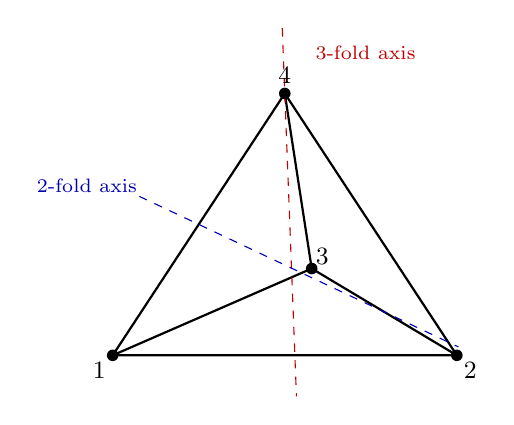
\begin{tikzpicture}[scale=1.9]
	\coordinate (A) at (-1.15,-0.6);
	\coordinate (B) at (1.15,-0.6);
	\coordinate (C) at (0.18,-0.02);
	\coordinate (D) at (0,1.15);
	\draw[thick] (A) -- (B) -- (D) -- cycle;
	\draw[thick] (A) -- (C) -- (B);
	\draw[thick] (C) -- (D);
	% 3-fold axis through D and the centroid of ABC
	\coordinate (M) at (0.06,-0.407);
	\draw[dashed, color=red!75!black] ($(D)!-0.28!(M)$) -- ($(D)!1.3!(M)$);
	% 2-fold axis through midpoints of AD and BC
	\coordinate (P) at (-0.575,0.275);
	\coordinate (Q) at (0.665,-0.31);
	\draw[dashed, color=blue!70!black] ($(P)!-0.32!(Q)$) -- ($(P)!1.4!(Q)$);
	\foreach \p in {A,B,C,D} \fill (\p) circle (1.1pt);
	\node[below left=-1pt] at (A) {\small $1$};
	\node[below right=-1pt] at (B) {\small $2$};
	\node[above right=-2pt] at (C) {\small $3$};
	\node[above] at (D) {\small $4$};
	\node[color=red!75!black, right] at (0.14,1.42) {\scriptsize $3$-fold axis};
	\node[color=blue!70!black, above left=-2pt] at (-0.96,0.46) {\scriptsize $2$-fold axis};
\end{tikzpicture}
\end{center}

The conjugacy classes of $S_4$ meeting $A_4$ are those of $e$, of $(1\,2)(3\,4)$, and of $(1\,2\,3)$; the first two remain single $A_4$-classes but the class of $3$-cycles splits in two, because $\Cent_{S_4}((1\,2\,3)) = \gen{(1\,2\,3)} \leq A_4$. So the classes of $A_4$ are
$$\{e\}\ (1),\qquad \{(1\,2)(3\,4),(1\,3)(2\,4),(1\,4)(2\,3)\}\ (3),\qquad \ccl((1\,2\,3))\ (4),\qquad \ccl((1\,3\,2))\ (4),$$
four classes in all. Geometrically the two classes of $3$-cycles are the rotations by $+2\pi/3$ and by $-2\pi/3$ about the four $3$-fold axes.

Now $A_4' = V_4$ (the double transpositions together with $e$), and $A_4/V_4\cong C_3$. So there are three linear characters, the lifts of the characters of $C_3$, and $12 = 1+1+1+d_4^2$ gives $d_4 = 3$. The degree-$3$ character is the standard character $\pi - \mathbf 1$ of the action on $\{1,2,3,4\}$, with $\pi = (4,0,1,1)$. Writing $\omega = e^{2\pi i/3}$:

\begin{center}
\renewcommand{\arraystretch}{1.3}
\setlength{\tabcolsep}{12pt}
\begin{tabular}{c|cccc}
\toprule
class size & $1$ & $3$ & $4$ & $4$\\
 & $e$ & $(1\,2)(3\,4)$ & $(1\,2\,3)$ & $(1\,3\,2)$\\
\midrule
$\mathbf 1$ & $1$ & $1$ & $1$ & $1$\\
$\chi_2$ & $1$ & $1$ & $\omega$ & $\omega^2$\\
$\chi_3$ & $1$ & $1$ & $\omega^2$ & $\omega$\\
$\chi_4$ & $3$ & $-1$ & $0$ & $0$\\
\bottomrule
\end{tabular}
\end{center}

Checks: degrees $1+1+1+9 = 12$. Rows: $\ip{\chi_4}{\chi_4} = \frac1{12}(9 + 3\cdot1 + 0 + 0) = 1$; $\ip{\mathbf1}{\chi_4} = \frac1{12}(3 - 3) = 0$; $\ip{\chi_2}{\chi_2} = \frac1{12}(1 + 3 + 4 + 4) = 1$; $\ip{\chi_2}{\chi_3} = \frac1{12}(1 + 3 + 4\overline\omega\,\omega^2 + 4\overline{\omega^2}\omega) = \frac1{12}(4 + 4\omega + 4\omega^2) = 0$ since $1 + \omega+\omega^2 = 0$; $\ip{\mathbf 1}{\chi_2} = \frac1{12}(1+3+4\omega+4\omega^2) = 0$. Columns: $12$, then $1+1+1+1 = 4 = 12/3$, then $1+1+1+0 = 3 = 12/4$ twice. All correct.

Note the character table shows immediately that $A_4$ is not simple: $\kernel\chi_2 = \{e\}\cup\ccl((1\,2)(3\,4)) = V_4$ is a proper nontrivial normal subgroup.

\subsection{The Symmetric Group \texorpdfstring{$S_4$}{S4}}

Let $G = S_4$, of order $24$, which is the rotation group of the cube: the four space diagonals are permuted, and this gives an isomorphism onto $S_4$.

\begin{center}
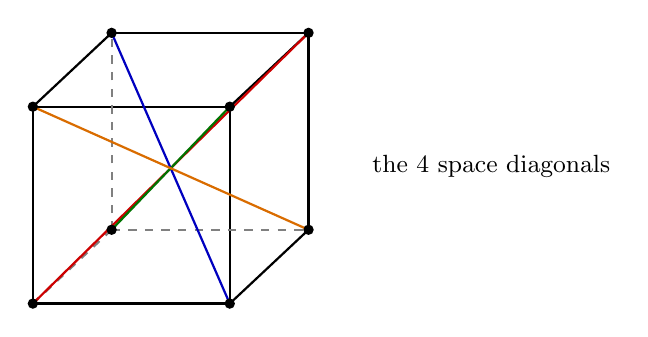
\begin{tikzpicture}[scale=1.25]
	\coordinate (a) at (0,0); \coordinate (b) at (2,0);
	\coordinate (c) at (2,2); \coordinate (d) at (0,2);
	\coordinate (e) at (0.8,0.75); \coordinate (f) at (2.8,0.75);
	\coordinate (g) at (2.8,2.75); \coordinate (h) at (0.8,2.75);
	\draw[thick] (a)--(b)--(c)--(d)--cycle;
	\draw[thick] (f)--(g)--(h);
	\draw[thick, dashed, gray] (e)--(f); \draw[thick, dashed, gray] (e)--(h);
	\draw[thick] (b)--(f); \draw[thick] (c)--(g); \draw[thick] (d)--(h);
	\draw[thick, dashed, gray] (a)--(e);
	% diagonals
	\draw[color=red!80!black, thick] (a)--(g);
	\draw[color=blue!75!black, thick] (b)--(h);
	\draw[color=green!45!black, thick] (c)--(e);
	\draw[color=orange!85!black, thick] (d)--(f);
	\foreach \p in {a,b,c,d,e,f,g,h} \fill (\p) circle (1.5pt);
	\node[right] at (3.35,1.4) {\small the $4$ space diagonals};
\end{tikzpicture}
\end{center}

The classes are indexed by cycle types: $e$ (size $1$), transpositions (size $6$), double transpositions (size $3$), $3$-cycles (size $8$), $4$-cycles (size $6$). Five classes, and $1+6+3+8+6 = 24$. Since $S_4' = A_4$, there are two linear characters $\mathbf 1$ and $\sign$, and
$$24 = 1 + 1 + d_3^2+d_4^2+d_5^2$$
with $d_i\geq 2$; the only solution is $\{2,3,3\}$.

We get the two degree-$3$ characters at once: $\chi_4 = \pi - \mathbf1$ is the standard character (irreducible since $S_4$ is $2$-transitive), and $\chi_5 = \sign\cdot\chi_4$ is another, distinct from $\chi_4$ since $\chi_4$ is not zero on transpositions. Here $\pi = (4,2,0,1,0)$, so $\chi_4 = (3,1,-1,0,-1)$ and $\chi_5 = (3,-1,-1,0,1)$.

The degree-$2$ character is the lift of the degree-$2$ character of $S_4/V_4\cong S_3$. Under the quotient map, $e$ and the double transpositions go to the identity, transpositions and $4$-cycles go to transpositions, and $3$-cycles go to $3$-cycles. Reading off from the table of $S_3$, we get $\chi_3 = (2,0,2,-1,0)$.

\begin{center}
\renewcommand{\arraystretch}{1.3}
\setlength{\tabcolsep}{10pt}
\begin{tabular}{c|ccccc}
\toprule
class size & $1$ & $6$ & $3$ & $8$ & $6$\\
 & $e$ & $(1\,2)$ & $(1\,2)(3\,4)$ & $(1\,2\,3)$ & $(1\,2\,3\,4)$\\
\midrule
$\mathbf 1$ & $1$ & $1$ & $1$ & $1$ & $1$\\
$\sign$ & $1$ & $-1$ & $1$ & $1$ & $-1$\\
$\chi_3$ & $2$ & $0$ & $2$ & $-1$ & $0$\\
$\chi_4$ & $3$ & $1$ & $-1$ & $0$ & $-1$\\
$\chi_5$ & $3$ & $-1$ & $-1$ & $0$ & $1$\\
\bottomrule
\end{tabular}
\end{center}

Let us check this properly.
\begin{itemize}
	\item Degrees: $1+1+4+9+9 = 24 = |S_4|$.
	\item $\ip{\chi_3}{\chi_3} = \frac1{24}(1\cdot4 + 6\cdot 0 + 3\cdot 4 + 8\cdot 1 + 6\cdot 0) = \frac{24}{24}=1$.
	\item $\ip{\chi_4}{\chi_4} = \frac1{24}(9 + 6 + 3 + 0 + 6) = \frac{24}{24}=1$, and by symmetry $\ip{\chi_5}{\chi_5} = 1$.
	\item $\ip{\mathbf1}{\sign} = \frac1{24}(1 - 6 + 3 + 8 - 6) = 0$; \; $\ip{\mathbf1}{\chi_3} = \frac1{24}(2 + 0 + 6 - 8 + 0) = 0$; \; $\ip{\mathbf1}{\chi_4} = \frac1{24}(3 + 6 - 3 + 0 - 6) = 0$; \; $\ip{\mathbf1}{\chi_5} = \frac1{24}(3-6-3+0+6) = 0$.
	\item $\ip{\sign}{\chi_3} = \frac1{24}(2 - 0 + 6 - 8 - 0) = 0$; \; $\ip{\sign}{\chi_4} = \frac1{24}(3 - 6 - 3 + 0 + 6) = 0$; \; $\ip{\sign}{\chi_5} = \frac1{24}(3 + 6 - 3 + 0 - 6) = 0$.
	\item $\ip{\chi_3}{\chi_4} = \frac1{24}(6 + 0 - 6 + 0 + 0) = 0$; \; $\ip{\chi_3}{\chi_5} = \frac1{24}(6 - 0 - 6 + 0 + 0) = 0$; \; $\ip{\chi_4}{\chi_5} = \frac1{24}(9 - 6 + 3 + 0 - 6) = 0$.
	\item Columns: $e$: $1+1+4+9+9 = 24$. \;$(1\,2)$: $1+1+0+1+1 = 4 = 24/6$. \;$(1\,2)(3\,4)$: $1+1+4+1+1 = 8 = 24/3$. \;$(1\,2\,3)$: $1+1+1+0+0 = 3 = 24/8$. \;$(1\,2\,3\,4)$: $1+1+0+1+1 = 4 = 24/6$.
\end{itemize}
Every relation holds, so the table is correct.

\begin{remark}
	As a sanity check on $\chi_3$: earlier we computed the permutation character of $S_4$ on the six unordered pairs to be $\pi_X = (6,2,2,0,0)$, and found $\ip{\pi_X}{\pi_X}=3$ with $\ip{\pi_X}{\mathbf 1}=1$. Indeed
	$$\pi_X = \mathbf 1 + \chi_3 + \chi_4 = (1,1,1,1,1)+(2,0,2,-1,0)+(3,1,-1,0,-1) = (6,2,2,0,0). \checkmark$$
\end{remark}

\subsection{The Alternating Group \texorpdfstring{$A_5$}{A5}}

Now for the most interesting small example. $A_5$ has order $60$ and is the rotation group of the regular icosahedron (equivalently, of the dodecahedron).

\begin{center}
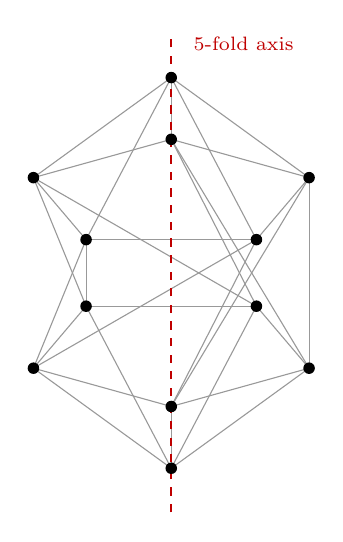
\begin{tikzpicture}[scale=1.6]
	\coordinate (T) at (0,1.55);
	\coordinate (B) at (0,-1.55);
	\foreach \i in {0,...,4} {
		\pgfmathsetmacro{\ang}{90 + 72*\i}
		\coordinate (U\i) at ({1.15*cos(\ang)}, {0.62 + 0.44*sin(\ang)});
		\pgfmathsetmacro{\angl}{54 + 72*\i}
		\coordinate (L\i) at ({1.15*cos(\angl)}, {-0.62 + 0.44*sin(\angl)});
	}
	\foreach \i in {0,...,4} {
		\pgfmathtruncatemacro{\j}{mod(\i+1,5)}
		\draw[thin, gray!80] (U\i) -- (U\j);
		\draw[thin, gray!80] (L\i) -- (L\j);
		\draw[thin, gray!80] (T) -- (U\i);
		\draw[thin, gray!80] (B) -- (L\i);
		\draw[thin, gray!80] (U\i) -- (L\i);
		\draw[thin, gray!80] (U\j) -- (L\i);
	}
	\draw[dashed, color=red!75!black, thick] (0,-1.9) -- (0,1.9);
	\foreach \i in {0,...,4} { \fill (U\i) circle (1.3pt); \fill (L\i) circle (1.3pt); }
	\fill (T) circle (1.3pt); \fill (B) circle (1.3pt);
	\node[color=red!75!black, right] at (0.1,1.82) {\scriptsize $5$-fold axis};
\end{tikzpicture}
\end{center}

The conjugacy classes of $A_5$ are those of $e$, of $(1\,2)(3\,4)$, of $(1\,2\,3)$, and \emph{two} classes of $5$-cycles. (The class of $5$-cycles in $S_5$ has $24$ elements and splits, since $\Cent_{S_5}((1\,2\,3\,4\,5)) = \gen{(1\,2\,3\,4\,5)}\leq A_5$; the classes of $(1\,2)(3\,4)$ and $(1\,2\,3)$ do not split, as $(1\,2)$ and $(4\,5)$ respectively centralise a representative while lying outside $A_5$.) Sizes:
$$1,\quad 15,\quad 20,\quad 12,\quad 12, \qquad \text{summing to } 60.$$
Geometrically these are: the identity; the $15$ rotations by $\pi$ about the $15$ edge-midpoint axes; the $20$ rotations by $\pm2\pi/3$ about the $10$ face axes; and the $24$ rotations by $\pm2\pi/5$ and $\pm4\pi/5$ about the $6$ vertex axes, splitting $12+12$.

$A_5$ is perfect, so $\mathbf 1$ is the only linear character, and $60 = 1 + d_2^2+d_3^2+d_4^2+d_5^2$ with $d_i\geq 2$ and (as we shall prove later) each $d_i$ dividing $60$. Let us instead just build characters.

\textbf{Degree $4$.} $A_5$ is $2$-transitive on $\{1,\dots,5\}$, so $\chi_4 := \pi - \mathbf 1$ is irreducible of degree $4$, where $\pi = (5,1,2,0,0)$. Thus $\chi_4 = (4,0,1,-1,-1)$.

\textbf{Degree $5$.} Compute the symmetric square. We need $\chi_4(g^2)$: for $g = e$ or a double transposition, $g^2 = e$ so $\chi_4(g^2) = 4$; for a $3$-cycle, $g^2$ is a $3$-cycle so $\chi_4(g^2) = 1$; and for a $5$-cycle $g$, $g^2$ is a $5$-cycle in the \emph{other} class, but $\chi_4$ takes the value $-1$ on both, so $\chi_4(g^2) = -1$. Hence
$$\chi_{S^2}(g) = \tfrac12(\chi_4(g)^2 + \chi_4(g^2)) = (10, 2, 1, 0, 0).$$
Now $\ip{\chi_{S^2}}{\mathbf 1} = \frac1{60}(10 + 15\cdot2 + 20\cdot 1 + 0 + 0) = 1$ and $\ip{\chi_{S^2}}{\chi_4} = \frac1{60}(40 + 0 + 20 + 0 + 0) = 1$. So
$$\chi_5 := \chi_{S^2} - \mathbf 1 - \chi_4 = (5,1,-1,0,0),$$
and $\ip{\chi_5}{\chi_5} = \frac1{60}(25 + 15 + 20 + 0 + 0) = 1$: irreducible, of degree $5$.

\textbf{Degree $3$, twice.} Compute the exterior square:
$$\chi_{\Lambda^2}(g) = \tfrac12(\chi_4(g)^2 - \chi_4(g^2)) = (6,-2,0,1,1).$$
Then $\ip{\chi_{\Lambda^2}}{\chi_{\Lambda^2}} = \frac1{60}(36 + 15\cdot 4 + 0 + 12 + 12) = \frac{120}{60} = 2$, so it is a sum of two distinct irreducibles; and it is orthogonal to $\mathbf 1$ and to $\chi_4$ (check: $\frac1{60}(6 - 30 + 0 + 12+12) = 0$ and $\frac1{60}(24 + 0 + 0 - 12 - 12) = 0$) and to $\chi_5$ (check: $\frac1{60}(30 - 30 + 0 + 0 + 0) = 0$). So $\chi_{\Lambda^2} = \chi_2 + \chi_3$ for two new irreducibles of degrees summing to $6$; since $60 = 1 + 16+25+d_2^2+d_3^2$ gives $d_2^2+d_3^2 = 18$ with $d_2+d_3 = 6$, we get $d_2 = d_3 = 3$.

To find the entries, write $\chi_2 = (3,a,b,c,c')$ and $\chi_3 = (3,\tilde a,\tilde b,\tilde c,\tilde c')$ with $\chi_2+\chi_3 = (6,-2,0,1,1)$. Column orthogonality gives, for the class of $(1\,2)(3\,4)$ (centraliser order $60/15 = 4$),
$$1 + a^2+\tilde a^2 + 0^2 + 1^2 = 4 \implies a^2 + \tilde a^2 = 2, \quad a + \tilde a = -2 \implies a = \tilde a = -1.$$
For the class of $(1\,2\,3)$ (centraliser order $3$): $1 + b^2+\tilde b^2 + 1 + 1 = 3$, so $b = \tilde b = 0$. For the class of $(1\,2\,3\,4\,5)$ (centraliser order $5$): $1 + c^2 + \tilde c^2 + 1 + 0 = 5$, so $c^2+\tilde c^2 = 3$ while $c + \tilde c = 1$; hence $c\tilde c = \frac12((c+\tilde c)^2 - (c^2+\tilde c^2)) = -1$, so $c,\tilde c$ are the roots of $x^2 - x - 1 = 0$, that is
$$\alpha = \frac{1+\sqrt5}{2}, \qquad \beta = \frac{1-\sqrt5}{2}.$$
The same holds on the other class of $5$-cycles, with the two values swapped (they must be, or $\chi_2 = \chi_3$).

\begin{center}
\renewcommand{\arraystretch}{1.35}
\setlength{\tabcolsep}{9pt}
\begin{tabular}{c|ccccc}
\toprule
class size & $1$ & $15$ & $20$ & $12$ & $12$\\
 & $e$ & $(1\,2)(3\,4)$ & $(1\,2\,3)$ & $(1\,2\,3\,4\,5)$ & $(1\,3\,5\,2\,4)$\\
\midrule
$\mathbf 1$ & $1$ & $1$ & $1$ & $1$ & $1$\\
$\chi_2$ & $3$ & $-1$ & $0$ & $\alpha$ & $\beta$\\
$\chi_3$ & $3$ & $-1$ & $0$ & $\beta$ & $\alpha$\\
$\chi_4$ & $4$ & $0$ & $1$ & $-1$ & $-1$\\
$\chi_5$ & $5$ & $1$ & $-1$ & $0$ & $0$\\
\bottomrule
\end{tabular}
\end{center}
where $\alpha = \frac{1+\sqrt5}2$ and $\beta = \frac{1-\sqrt5}2$, so that $\alpha+\beta = 1$, $\alpha\beta = -1$ and $\alpha^2+\beta^2 = 3$.

Let us verify everything, using these three identities.
\begin{itemize}
	\item Degrees: $1 + 9 + 9 + 16 + 25 = 60 = |A_5|$.
	\item $\ip{\chi_2}{\chi_2} = \frac1{60}(9 + 15 + 0 + 12\alpha^2 + 12\beta^2) = \frac{9+15+36}{60} = 1$; same for $\chi_3$.
	\item $\ip{\chi_4}{\chi_4} = \frac1{60}(16 + 0 + 20 + 12 + 12) = 1$; \; $\ip{\chi_5}{\chi_5} = \frac1{60}(25 + 15 + 20 + 0 + 0) = 1$.
	\item $\ip{\chi_2}{\chi_3} = \frac1{60}(9 + 15 + 0 + 12\alpha\beta + 12\beta\alpha) = \frac{9+15-24}{60} = 0$.
	\item $\ip{\mathbf1}{\chi_2} = \frac1{60}(3 - 15 + 0 + 12\alpha + 12\beta) = \frac{3-15+12}{60}=0$; same for $\chi_3$.
	\item $\ip{\mathbf1}{\chi_4} = \frac1{60}(4+0+20-12-12) = 0$; \; $\ip{\mathbf1}{\chi_5} = \frac1{60}(5+15-20+0+0)=0$.
	\item $\ip{\chi_2}{\chi_4} = \frac1{60}(12 + 0 + 0 - 12\alpha - 12\beta) = \frac{12-12}{60} = 0$; same for $\chi_3$.
	\item $\ip{\chi_2}{\chi_5} = \frac1{60}(15 - 15 + 0 + 0 + 0)=0$; same for $\chi_3$; \; $\ip{\chi_4}{\chi_5} = \frac1{60}(20 + 0 - 20 + 0 + 0) = 0$.
	\item Columns: $e$: $1+9+9+16+25 = 60$. \;$(1\,2)(3\,4)$: $1+1+1+0+1 = 4 = 60/15$. \;$(1\,2\,3)$: $1+0+0+1+1 = 3 = 60/20$. \;Each $5$-class: $1 + \alpha^2+\beta^2+1+0 = 1+3+1 = 5 = 60/12$.
\end{itemize}

Finally, the table shows that $A_5$ is simple: for each $i\neq 1$ and each $g\neq e$ we have $\chi_i(g)\neq\chi_i(e)$, since the entries $-1,0,\alpha,\beta,1$ are never equal to $3,4$ or $5$. So no proper nontrivial normal subgroup exists.

\begin{remark}
	The appearance of the golden ratio is not a coincidence: the two degree-$3$ representations are the two ways of realising $A_5$ as the rotation group of the icosahedron (differing by the outer automorphism of $A_5$, which swaps the two classes of $5$-cycles), and the trace of a rotation by $2\pi/5$ in $\R^3$ is $1 + 2\cos(2\pi/5) = \frac{1+\sqrt5}{2} = \alpha$.
\end{remark}

\subsection{The Symmetric Group \texorpdfstring{$S_5$}{S5}}

Finally $S_5$, of order $120$, which has seven conjugacy classes, indexed by cycle type:
$$\begin{array}{lccccccc}
\text{type} & 1^5 & 2\,1^3 & 2^2 1 & 3\,1^2 & 3\,2 & 4\,1 & 5\\
\text{size} & 1 & 10 & 15 & 20 & 20 & 30 & 24
\end{array}$$
(these sum to $120$). Since $S_5' = A_5$, there are two linear characters. Let $\pi = (5,3,1,2,0,1,0)$ be the natural permutation character, so the standard character is
$$\chi_3 = \pi - \mathbf 1 = (4,2,0,1,-1,0,-1),$$
irreducible by $2$-transitivity, and $\chi_4 = \sign\cdot\chi_3 = (4,-2,0,1,1,0,-1)$ is a second one of degree $4$.

For more, take squares of $\chi_3$. We need the class of $g^2$ for each $g$: $e,(1\,2),(1\,2)(3\,4)$ all square into $1^5$; $(1\,2\,3)$ and $(1\,2\,3)(4\,5)$ square to $3$-cycles; $(1\,2\,3\,4)$ squares to a $2^2$-element; and a $5$-cycle squares to a $5$-cycle. Hence
$$\chi_3(g^2) = (4,4,4,1,1,0,-1),$$
and so
\begin{align*}
	\chi_{S^2}(g) &= \tfrac12\big(\chi_3(g)^2+\chi_3(g^2)\big) = (10,4,2,1,1,0,0),\\
	\chi_{\Lambda^2}(g) &= \tfrac12\big(\chi_3(g)^2-\chi_3(g^2)\big) = (6,0,-2,0,0,0,1).
\end{align*}
Now $\ip{\chi_{\Lambda^2}}{\chi_{\Lambda^2}} = \frac1{120}(36 + 0 + 15\cdot4+0+0+0+24) = \frac{120}{120} = 1$, so $\chi_5 := \chi_{\Lambda^2}$ is irreducible of degree $6$. (Note $\sign\cdot\chi_5 = \chi_5$: this character is `self-associate'.)

For the symmetric square, $\ip{\chi_{S^2}}{\mathbf 1} = \frac1{120}(10+40+30+20+20+0+0) = 1$ and $\ip{\chi_{S^2}}{\chi_3} = \frac1{120}(40 + 80 + 0 + 20 - 20 + 0 + 0) = 1$, so
$$\chi_6 := \chi_{S^2} - \mathbf 1 - \chi_3 = (5,1,1,-1,1,-1,0),$$
with $\ip{\chi_6}{\chi_6} = \frac1{120}(25 + 10 + 15 + 20 + 20 + 30 + 0) = 1$: irreducible of degree $5$. And $\chi_7 = \sign\cdot\chi_6 = (5,-1,1,-1,-1,1,0)$ is a seventh, distinct from $\chi_6$. Degrees: $1+1+16+16+25+25+36 = 120$, so we have them all.

\begin{center}
\renewcommand{\arraystretch}{1.35}
\setlength{\tabcolsep}{7pt}
\begin{tabular}{c|ccccccc}
\toprule
class size & $1$ & $10$ & $15$ & $20$ & $20$ & $30$ & $24$\\
 & $e$ & $(1\,2)$ & $(1\,2)(3\,4)$ & $(1\,2\,3)$ & $(1\,2\,3)(4\,5)$ & $(1\,2\,3\,4)$ & $(1\,2\,3\,4\,5)$\\
\midrule
$\mathbf 1$ & $1$ & $1$ & $1$ & $1$ & $1$ & $1$ & $1$\\
$\sign$ & $1$ & $-1$ & $1$ & $1$ & $-1$ & $-1$ & $1$\\
$\chi_3$ & $4$ & $2$ & $0$ & $1$ & $-1$ & $0$ & $-1$\\
$\chi_4$ & $4$ & $-2$ & $0$ & $1$ & $1$ & $0$ & $-1$\\
$\chi_5$ & $6$ & $0$ & $-2$ & $0$ & $0$ & $0$ & $1$\\
$\chi_6$ & $5$ & $1$ & $1$ & $-1$ & $1$ & $-1$ & $0$\\
$\chi_7$ & $5$ & $-1$ & $1$ & $-1$ & $-1$ & $1$ & $0$\\
\bottomrule
\end{tabular}
\end{center}

Verification of the column relations, which is the quickest global check:
$$\begin{array}{ll}
e: & 1+1+16+16+36+25+25 = 120 = |\Cent(e)|,\\
(1\,2): & 1+1+4+4+0+1+1 = 12 = 120/10,\\
(1\,2)(3\,4): & 1+1+0+0+4+1+1 = 8 = 120/15,\\
(1\,2\,3): & 1+1+1+1+0+1+1 = 6 = 120/20,\\
(1\,2\,3)(4\,5): & 1+1+1+1+0+1+1 = 6 = 120/20,\\
(1\,2\,3\,4): & 1+1+0+0+0+1+1 = 4 = 120/30,\\
(1\,2\,3\,4\,5): & 1+1+1+1+1+0+0 = 5 = 120/24.
\end{array}$$
And a sample of the row relations: $\ip{\chi_3}{\chi_4} = \frac1{120}(16 - 40 + 0 + 20 - 20 + 0 + 24) = 0$; $\ip{\chi_6}{\chi_7} = \frac1{120}(25 - 10 + 15 + 20 - 20 - 30 + 0) = 0$; $\ip{\chi_3}{\chi_5} = \frac1{120}(24 + 0 + 0 + 0 + 0 + 0 - 24) = 0$; $\ip{\chi_5}{\chi_6} = \frac1{120}(30 + 0 - 30 + 0+0+0+0) = 0$; $\ip{\mathbf 1}{\chi_5} = \frac1{120}(6 + 0 - 30 + 0 + 0 + 0 + 24) = 0$. (All twenty-one orthogonality relations hold; the reader is invited to spot-check a few more.)

\begin{remark}
	Notice the shape of the answer: seven irreducible characters, in three `associate pairs' $\{\mathbf1,\sign\}$, $\{\chi_3,\chi_4\}$, $\{\chi_6,\chi_7\}$ swapped by tensoring with $\sign$, and one self-associate character $\chi_5$. There is a beautiful combinatorial explanation in terms of partitions of $5$ and their transposes, which we come to in the section on the symmetric group.
\end{remark}

\section{Restriction and Induction}

So far all our constructions have taken place inside a fixed group. We now allow ourselves to move between a group and its subgroups, which turns out to be the single most powerful technique for building character tables of larger groups.

Throughout this section $H \leq G$ is a subgroup of index $n = |G:H|$.

\subsection{Restriction}

This direction is trivial to define and surprisingly informative.

\begin{definition}[Restriction]
	Let $(\rho, V)$ be a representation of $G$ and $H\leq G$. The \vocab{restriction} $\Res^G_H V$ (also written $V\!\downarrow_H$) is the representation of $H$ on the same space $V$ given by $\rho|_H$. On characters, $\Res^G_H\chi$ is just $\chi|_H$.
\end{definition}

Restricting an irreducible representation of $G$ to $H$ almost never gives an irreducible representation of $H$, but the failure is controlled.

\begin{proposition}
	Let $V$ be an irreducible representation of $G$ with character $\chi$, and write $\Res^G_H\chi = \sum_i c_i\psi_i$ over the irreducible characters $\psi_i$ of $H$. Then
	$$\sum_i c_i^2 = \ip{\Res^G_H\chi}{\Res^G_H\chi}_H \leq |G:H|,$$
	with equality if and only if $\chi(g) = 0$ for every $g \in G\setminus H$.
\end{proposition}
\begin{proof}
	We have
	$$\ip{\chi|_H}{\chi|_H}_H = \frac1{|H|}\sum_{h\in H}|\chi(h)|^2 = \frac{|G|}{|H|}\cdot\frac1{|G|}\sum_{h\in H}|\chi(h)|^2 \leq |G:H|\cdot\frac1{|G|}\sum_{g\in G}|\chi(g)|^2 = |G:H|,$$
	since $\ip\chi\chi_G = 1$. The inequality is an equality exactly when the omitted terms $|\chi(g)|^2$, $g\notin H$, all vanish.
\end{proof}

\begin{corollary}
	If $\chi$ is irreducible of degree $d$ and $H\leq G$ has index $n$, then $\Res^G_H\chi$ has at most $n$ irreducible constituents counted with multiplicity, and in particular $d \leq n\cdot\max_i\psi_i(1)$.
\end{corollary}

\begin{example}
	Restrict the degree-$2$ character $\chi = (2,0,-1)$ of $S_3$ to $H = A_3 = C_3$. We get $\chi|_H = (2,-1,-1)$ on $(e, (1\,2\,3),(1\,3\,2))$, which is $\omega + \omega^2$-flavoured: indeed $\chi|_H = \chi_1 + \chi_2$, the two nontrivial characters of $C_3$. Here $\ip{\chi|_H}{\chi|_H} = 2 = |G:H|$, consistent with $\chi$ vanishing off $A_3$.
\end{example}

\subsection{Induction}

The other direction is the interesting one: from a representation of $H$ we manufacture a representation of $G$, of degree multiplied by $|G:H|$.

Choose left coset representatives $g_1 = e, g_2,\dots,g_n$ for $H$ in $G$, so that $G = \bigsqcup_{i=1}^n g_iH$.

\begin{center}
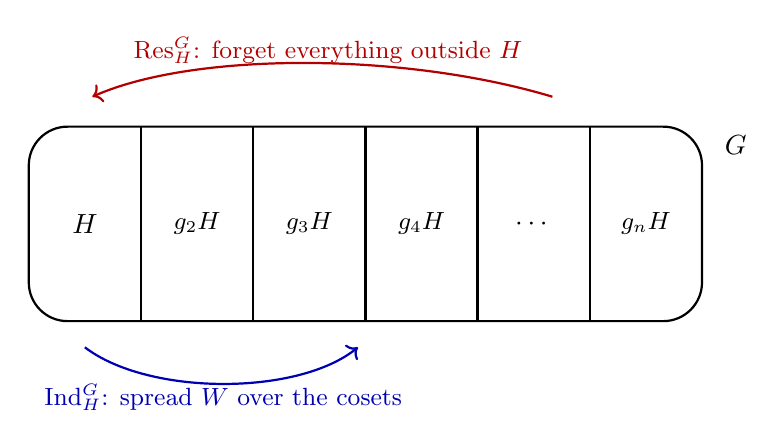
\begin{tikzpicture}[scale=0.95]
	\draw[rounded corners=14pt, thick] (0,0) rectangle (9,2.6);
	\node at (9.45,2.35) {$G$};
	\foreach \x in {1.5,3,4.5,6,7.5} {\draw[thick] (\x,0) -- (\x,2.6);}
	\node at (0.75,1.3) {$H$};
	\node at (2.25,1.3) {\small $g_2H$};
	\node at (3.75,1.3) {\small $g_3H$};
	\node at (5.25,1.3) {\small $g_4H$};
	\node at (6.75,1.3) {$\cdots$};
	\node at (8.25,1.3) {\small $g_nH$};
	% arrows
	\draw[->, thick, color=blue!70!black] (0.75,-0.35) .. controls (1.6,-1.0) and (3.6,-1.0) .. (4.4,-0.35);
	\node[color=blue!70!black] at (2.6,-1.02) {\small $\Ind_H^G$: spread $W$ over the cosets};
	\draw[->, thick, color=red!70!black] (7.0,3.0) .. controls (5.0,3.6) and (2.2,3.6) .. (0.85,3.0);
	\node[color=red!70!black] at (4.0,3.62) {\small $\Res^G_H$: forget everything outside $H$};
\end{tikzpicture}
\end{center}
\vspace{1.4em}

\begin{definition}[Induced representation]
	Let $W$ be a representation of $H$. The \vocab{induced representation} is the vector space
	$$\Ind_H^GW = \bigoplus_{i=1}^n g_i\otimes W,$$
	where $g_i\otimes W$ is a copy of $W$ labelled by the coset $g_iH$, with $G$ acting as follows: given $g \in G$ and $i$, write $g g_i = g_j h$ with $h \in H$ (which determines $j$ and $h$ uniquely), and set
	$$g\cdot(g_i\otimes w) = g_j\otimes hw.$$
	Its degree is $|G:H|\cdot\dim W$.
\end{definition}

\begin{remark}
	Invariantly, $\Ind_H^GW = \C G\otimes_{\C H}W$, the extension of scalars along $\C H\hookrightarrow\C G$; this makes the independence of the choice of coset representatives obvious, and identifies induction as the left adjoint of restriction. Readers who found tensor products of modules congenial in \emph{Groups, Rings and Modules} may prefer this definition; the concrete one above is what we compute with.
\end{remark}

One should check this is a representation. If $g' g_j = g_k h'$ then $g'g\,g_i = g'g_jh = g_kh'h$, so
$$g'\cdot(g\cdot(g_i\otimes w)) = g'\cdot (g_j\otimes hw) = g_k\otimes h'hw = (g'g)\cdot(g_i\otimes w),$$
as required, and the identity acts trivially.

\begin{theorem}[Induced character formula]
	Let $\psi$ be the character of a representation $W$ of $H\leq G$. Then the character of $\Ind_H^GW$ is
	$$\Ind_H^G\psi\,(g) = \sum_{\substack{1\leq i\leq n \\ g_i^{-1}gg_i\in H}}\psi\big(g_i^{-1}gg_i\big) \; = \; \frac1{|H|}\sum_{\substack{x\in G\\ x^{-1}gx\in H}}\psi\big(x^{-1}gx\big).$$
	In particular $\Ind_H^G\psi\,(e) = |G:H|\,\psi(e)$, and $\Ind_H^G\psi(g) = 0$ if no conjugate of $g$ lies in $H$.
\end{theorem}
\begin{proof}
	Write the matrix of $g$ in a basis adapted to the decomposition $\bigoplus_i g_i\otimes W$, as an $n\times n$ array of blocks of size $\dim W$. The action sends the $i$-th block into the $j$-th block, where $gg_i \in g_jH$. So the $(i,i)$ diagonal block is nonzero only when $gg_i\in g_iH$, i.e. $g_i^{-1}gg_i\in H$, and then it is the matrix of $\rho_W(g_i^{-1}gg_i)$. Taking traces of the diagonal blocks gives the first formula.

	For the second, every $x\in G$ is uniquely $x = g_ih$ with $h\in H$, and
	$$x^{-1}gx = h^{-1}(g_i^{-1}gg_i)h,$$
	which lies in $H$ if and only if $g_i^{-1}gg_i$ does, and then has the same $\psi$-value since $\psi$ is a class function on $H$. So each term of the first sum is repeated exactly $|H|$ times in the second.
\end{proof}

There is a third form of the formula which is often the most efficient for hand computation.

\begin{corollary}
	Let $g \in G$ and suppose $\ccl_G(g)\cap H$ is the disjoint union of the $H$-conjugacy classes of $h_1,\dots,h_m$ (possibly $m = 0$). Then
	$$\Ind_H^G\psi\,(g) = |\Cent_G(g)|\sum_{k=1}^m\frac{\psi(h_k)}{|\Cent_H(h_k)|}.$$
\end{corollary}
\begin{proof}
	In the sum $\frac1{|H|}\sum_{x: x^{-1}gx\in H}\psi(x^{-1}gx)$, group the $x$ by the value of $x^{-1}gx$. For a fixed $h\in\ccl_G(g)\cap H$, the number of $x$ with $x^{-1}gx = h$ is $|\Cent_G(g)|$. So the sum is $\frac{|\Cent_G(g)|}{|H|}\sum_{h\in\ccl_G(g)\cap H}\psi(h)$, and grouping the $h$ into $H$-classes of sizes $|H|/|\Cent_H(h_k)|$ gives the result.
\end{proof}

\subsection{Frobenius Reciprocity}

Restriction and induction are adjoint to one another, and this single fact organises everything.

\begin{theorem}[Frobenius reciprocity]
	Let $H\leq G$, let $\psi$ be a class function on $H$ and $\chi$ a class function on $G$. Then
	$$\ip{\Res^G_H\chi}{\psi}_H = \ip{\chi}{\Ind_H^G\psi}_G.$$
\end{theorem}
\begin{proof}
	Extend $\Ind_H^G$ to all class functions on $H$ by the formula of the theorem above (which makes sense for any class function). Then
	\begin{align*}
		\ip{\chi}{\Ind_H^G\psi}_G &= \frac1{|G|}\sum_{g\in G}\overline{\chi(g)}\cdot\frac1{|H|}\sum_{\substack{x\in G\\x^{-1}gx\in H}}\psi(x^{-1}gx)\\
		&= \frac1{|G||H|}\sum_{x\in G}\ \sum_{\substack{g\in G\\ x^{-1}gx\in H}}\overline{\chi(g)}\,\psi(x^{-1}gx).
	\end{align*}
	For fixed $x$, substitute $h = x^{-1}gx$; as $g$ runs over those elements of $G$ with $x^{-1}gx\in H$, $h$ runs over $H$, and $\chi(g) = \chi(xhx^{-1}) = \chi(h)$ since $\chi$ is a class function on $G$. So the inner sum is $\sum_{h\in H}\overline{\chi(h)}\psi(h)$, independent of $x$. Hence
	$$\ip\chi{\Ind_H^G\psi}_G = \frac{|G|}{|G||H|}\sum_{h\in H}\overline{\chi(h)}\psi(h) = \ip{\Res^G_H\chi}{\psi}_H. \qedhere$$
\end{proof}

\begin{corollary}
	$\Ind_H^G\psi$ is a character of $G$ whenever $\psi$ is a character of $H$, and induction takes nonnegative integer combinations of irreducible characters to nonnegative integer combinations.
\end{corollary}
\begin{proof}
	We constructed the induced representation, so this is automatic; but note it also follows formally, since $\ip{\chi_i}{\Ind\psi} = \ip{\Res\chi_i}{\psi} \geq 0$ is a nonnegative integer for every irreducible $\chi_i$.
\end{proof}

\begin{corollary}
	If $H \leq G$ and $\psi$ is an irreducible character of $H$, then every irreducible constituent of $\Ind_H^G\psi$ has $\psi$ as a constituent of its restriction to $H$, and vice versa.
\end{corollary}

\begin{example}[Permutation characters are induced]
	Let $G$ act transitively on $X$ and let $H = \stab_G(x_0)$. Then $\C X \cong \Ind_H^G\mathbf 1_H$: both have the same character, since
	$$\Ind_H^G\mathbf 1(g) = \frac{1}{|H|}\big|\{x\in G : x^{-1}gx\in H\}\big| = \big|\{xH : gxH = xH\}\big| = |\operatorname{fix}_X(g)|,$$
	using the identification $X \leftrightarrow G/H$. Frobenius reciprocity then reproves that $\ip{\pi_X}{\mathbf 1_G} = \ip{\mathbf1_H}{\mathbf 1_H} = 1$ for transitive actions.
\end{example}

\begin{example}[The two-dimensional character of $D_8$]
	Take $G = D_8$ and $H = \gen r\cong C_4$, of index $2$, with coset representatives $e, s$. Let $\psi(r^k) = i^k$ be a faithful character of $H$. Since $H$ is normal, every conjugate of $r^k$ lies in $H$, and
	$$\Ind_H^G\psi(r^k) = \psi(r^k) + \psi(s^{-1}r^ks) = i^k + i^{-k},$$
	which is $2, 0, -2, 0$ for $k = 0,1,2,3$; while for a reflection $g$, no conjugate lies in $H$, so $\Ind\psi(g) = 0$. Thus $\Ind_H^G\psi = (2,-2,0,0,0)$ on the classes $e, r^2, r, s, rs$ -- exactly the degree-$2$ irreducible character of $D_8$. This is how one builds the dihedral characters `from above'.
\end{example}

\begin{example}[Building characters of $A_5$ by induction]
	Take $G = A_5$ and $H = A_4$, the stabiliser of the point $5$, of index $5$.

	Inducing the trivial character gives the permutation character on $5$ points, $(5,1,2,0,0) = \mathbf 1 + \chi_4$.

	Now induce the linear character $\psi = \chi_2$ of $A_4$, with values $(1,1,\omega,\omega^2)$ on the classes $e$, $(1\,2)(3\,4)$, $(1\,2\,3)$, $(1\,3\,2)$ of $A_4$. Use the centraliser form of the induced character formula, recalling $|\Cent_{A_5}|$ has values $60, 4, 3, 5, 5$ on the five classes of $A_5$, and $|\Cent_{A_4}|$ has values $12, 4, 3, 3$ on the classes of $A_4$.
	\begin{itemize}
		\item $g = e$: \; $\Ind\psi(e) = 60\cdot\frac{1}{12} = 5$, as it must be ($5 = |G:H|\cdot 1$).
		\item $g = (1\,2)(3\,4)$: the $A_5$-class of $g$ meets $A_4$ in the single $A_4$-class of double transpositions, so $\Ind\psi(g) = 4\cdot\frac{1}{4} = 1$.
		\item $g = (1\,2\,3)$: the $A_5$-class of $3$-cycles meets $A_4$ in \emph{two} $A_4$-classes, on which $\psi$ takes the values $\omega$ and $\omega^2$. So $\Ind\psi(g) = 3\big(\frac{\omega}{3}+\frac{\omega^2}{3}\big) = \omega+\omega^2 = -1$.
		\item $g$ a $5$-cycle: $A_4$ contains no elements of order $5$, so $\Ind\psi(g) = 0$.
	\end{itemize}
	Hence $\Ind_{A_4}^{A_5}\chi_2 = (5,1,-1,0,0) = \chi_5$, which we found earlier as $S^2\chi_4 - \mathbf 1-\chi_4$. Two different routes to the same character is always reassuring.
\end{example}

\begin{remark}[Transitivity of induction]
	If $K\leq H\leq G$ then $\Ind_H^G\Ind_K^H = \Ind_K^G$, and likewise $\Res$ is transitive. Both follow from Frobenius reciprocity: for any irreducible $\chi$ of $G$,
	$$\ip{\chi}{\Ind_H^G\Ind_K^H\psi} = \ip{\Res_H\chi}{\Ind_K^H\psi} = \ip{\Res_K\chi}{\psi} = \ip\chi{\Ind_K^G\psi}.$$
\end{remark}

\subsection{A Character Table Built by Induction}

Here is a complete worked example where induction is genuinely the only easy route. Let
$$G = C_7\rtimes C_3 = \gen{a, b \mid a^7 = b^3 = e,\ bab^{-1} = a^2},$$
a nonabelian group of order $21$. (Such a group exists because $2$ has order $3$ modulo $7$.)

\textbf{Conjugacy classes.} Conjugating $a$ by $b$ repeatedly gives $a\mapsto a^2\mapsto a^4\mapsto a^8 = a$, so $\{a,a^2,a^4\}$ is a class; similarly $\{a^3,a^6,a^5\}$ is a class. The elements $a^ib$ are all conjugate: since $\Cent_G(b)\supseteq\gen b$ has order at least $3$ and $b\notin Z(G)$, the class of $b$ has size dividing $7$ and greater than $1$, so exactly $7$; likewise for $b^2$. So the classes are
$$\{e\}\ (1),\quad \{a,a^2,a^4\}\ (3),\quad\{a^3,a^5,a^6\}\ (3),\quad \ccl(b)\ (7),\quad\ccl(b^2)\ (7),$$
totalling $1+3+3+7+7 = 21$. So there are five irreducible characters.

\textbf{Degrees.} We have $G' = \gen a$ (as $bab^{-1}a^{-1} = a$), so $G/G'\cong C_3$ and there are exactly three linear characters $\mathbf 1,\chi_2,\chi_3$, given by $a\mapsto1$, $b\mapsto\omega^{\pm1}$ with $\omega = e^{2\pi i/3}$. Then $21 = 3 + d_4^2+d_5^2$ gives $d_4 = d_5 = 3$.

\textbf{The degree-$3$ characters.} Take $H = \gen a\cong C_7$, of index $3$, and let $\zeta = e^{2\pi i/7}$ with $\psi(a^k) = \zeta^k$. Since $H\normal G$, every conjugate of an element of $H$ lies in $H$, and the coset representatives $e, b, b^2$ give
$$\Ind_H^G\psi\,(a^k) = \psi(a^k)+\psi(b^{-1}a^kb) + \psi(b^{-2}a^kb^2) = \zeta^k+\zeta^{4k}+\zeta^{2k},$$
using $b^{-1}ab = a^4$ and $b^{-2}ab^2 = a^2$. No conjugate of $b$ or $b^2$ lies in $H$, so $\Ind_H^G\psi$ vanishes there. Writing
$$\eta = \zeta+\zeta^2+\zeta^4, \qquad \overline\eta = \zeta^3+\zeta^5+\zeta^6,$$
(the sums over the quadratic residues and non-residues modulo $7$) we get $\Ind_H^G\psi = (3,\eta,\overline\eta,0,0)$. Note
$$\eta+\overline\eta = \sum_{k=1}^6\zeta^k = -1, \qquad \eta\,\overline\eta = 2.$$
The first is the vanishing of the sum of all seventh roots of unity other than $1$. For the second, expand into nine terms:
$$(\zeta+\zeta^2+\zeta^4)(\zeta^3+\zeta^5+\zeta^6) = \big(\zeta^4+\zeta^6+1\big)+\big(\zeta^5+1+\zeta\big)+\big(1+\zeta^2+\zeta^3\big) = 3 + \sum_{k=1}^6\zeta^k = 2.$$
So $\eta,\overline\eta$ are the roots of $x^2+x+2$, that is $\eta = \frac{-1+i\sqrt7}{2}$ (which is indeed the complex conjugate of $\overline\eta$, justifying the notation). Then
$$\ip{\Ind\psi}{\Ind\psi} = \frac1{21}\big(9 + 3|\eta|^2+3|\overline\eta|^2\big) = \frac{9+6+6}{21} = 1,$$
so $\chi_4 := \Ind_H^G\psi$ is irreducible; and $\chi_5 = \overline{\chi_4} = (3,\overline\eta,\eta,0,0)$ is a second one, obtained by inducing $\psi^3$ instead.

\begin{center}
\renewcommand{\arraystretch}{1.35}
\setlength{\tabcolsep}{11pt}
\begin{tabular}{c|ccccc}
\toprule
class size & $1$ & $3$ & $3$ & $7$ & $7$\\
 & $e$ & $a$ & $a^3$ & $b$ & $b^2$\\
\midrule
$\mathbf 1$ & $1$ & $1$ & $1$ & $1$ & $1$\\
$\chi_2$ & $1$ & $1$ & $1$ & $\omega$ & $\omega^2$\\
$\chi_3$ & $1$ & $1$ & $1$ & $\omega^2$ & $\omega$\\
$\chi_4$ & $3$ & $\eta$ & $\overline\eta$ & $0$ & $0$\\
$\chi_5$ & $3$ & $\overline\eta$ & $\eta$ & $0$ & $0$\\
\bottomrule
\end{tabular}
\end{center}
where $\eta = \frac{-1+i\sqrt7}{2}$, so $\eta+\overline\eta = -1$ and $\eta\overline\eta = 2$.

Checks: degrees $1+1+1+9+9 = 21$. Rows: $\ip{\chi_4}{\chi_4} = \frac1{21}(9+6+6) = 1$; $\ip{\chi_4}{\chi_5} = \frac1{21}(9 + 3\overline\eta^{\,2}+3\eta^2) = \frac{9 + 3(\eta^2+\overline\eta^2)}{21} = \frac{9+3(1-4)}{21} = 0$, using $\eta^2+\overline\eta^2 = (\eta+\overline\eta)^2 - 2\eta\overline\eta = -3$; $\ip{\mathbf1}{\chi_4} = \frac1{21}(3+3\eta+3\overline\eta) = 0$; $\ip{\chi_2}{\chi_4} = \frac1{21}(3+3\eta+3\overline\eta+0+0) = 0$; $\ip{\mathbf1}{\chi_2} = \frac1{21}(1+3+3+7\omega+7\omega^2) = \frac{7 - 7}{21} = 0$. Columns: $e$ gives $21$; $a$ gives $1+1+1+|\eta|^2+|\overline\eta|^2 = 3+2+2 = 7 = 21/3$, and likewise for $a^3$; $b$ gives $1+1+1+0+0 = 3 = 21/7$, and likewise for $b^2$. All correct.

\begin{remark}
	This $G$ is the smallest nonabelian group of odd order, and it is a Frobenius group: the complement is $\gen b\cong C_3$, which satisfies $\gen b\cap g\gen bg^{-1} = 1$ for $g\notin\gen b$, and the Frobenius kernel is $\gen a\cong C_7$. Frobenius' theorem below explains, from the characters alone, why $\gen a$ had to be normal.
\end{remark}

\subsection{Mackey's Formulae}

We record, without full proofs, the theorem which describes what happens when induction and restriction are composed the `wrong' way round. It is not needed in the sequel, but it is the natural completion of the story.

Let $H, K \leq G$. The set $K\backslash G/H$ of \vocab{double cosets} $KgH$ partitions $G$; each double coset is a union of left cosets of $H$. For $g \in G$, write $H^g = g^{-1}Hg$ and let ${}^gW$ denote the representation of $gHg^{-1}$ on $W$ given by $(ghg^{-1})\cdot w = hw$.

\begin{theorem}[Mackey's restriction formula]
	With notation as above, for a representation $W$ of $H$,
	$$\Res^G_K\Ind_H^GW \; \cong \; \bigoplus_{KgH\,\in\, K\backslash G/H}\Ind^K_{K\cap\, {}^gH}\Res^{{}^gH}_{K\cap\, {}^gH}\big({}^gW\big),$$
	where ${}^gH = gHg^{-1}$. The right hand side does not depend on the choice of double coset representatives.
\end{theorem}

The proof is a bookkeeping exercise: the space $\Ind_H^GW = \bigoplus_{xH}x\otimes W$ is permuted by $K$ according to the action of $K$ on $G/H$, whose orbits are exactly the double cosets, and one identifies the summand corresponding to each orbit.

\begin{corollary}[Mackey's irreducibility criterion]
	Let $H\leq G$ and $W$ an irreducible representation of $H$. Then $\Ind_H^GW$ is irreducible if and only if, for every $g \in G\setminus H$, the representations
	$$\Res^{H}_{H\cap\, {}^gH}W \qquad\text{and}\qquad \Res^{{}^gH}_{H\cap\, {}^gH}\big({}^gW\big)$$
	of $H\cap{}^gH$ have no irreducible constituent in common.
\end{corollary}
\begin{proof}[Proof sketch]
	By Frobenius reciprocity and Mackey with $K = H$,
	$$\ip{\Ind_H^GW}{\Ind_H^GW}_G = \ip{W}{\Res^G_H\Ind_H^GW}_H = \sum_{HgH}\ip{\Res_{H\cap{}^gH}W}{\Res_{H\cap{}^gH}({}^gW)}_{H\cap{}^gH}.$$
	The term for the double coset $H$ itself contributes $\ip WW_H = 1$, and all other terms are nonnegative; so the total is $1$ if and only if all the others vanish.
\end{proof}

\begin{corollary}
	If $H\normal G$ and $W$ is irreducible, then $\Ind_H^GW$ is irreducible if and only if ${}^gW\not\cong W$ for all $g\in G\setminus H$.
\end{corollary}

\subsection{An Application: Frobenius' Theorem}

Here is a striking theorem which cannot (to this day) be proved without characters. It is the reason induction earns its keep.

\begin{definition}[Frobenius group]
	Let $G$ be a finite group with a subgroup $1 < H < G$ such that
	$$H\cap gHg^{-1} = 1\qquad\text{for all } g\in G\setminus H.$$
	We call $H$ a \vocab{Frobenius complement} and $G$ a \vocab{Frobenius group}.
\end{definition}

Equivalently, $G$ acts transitively on $G/H$ in such a way that no nonidentity element fixes two points, but some nonidentity element fixes a point.

\begin{theorem}[Frobenius, 1901]
	Let $G$ be a Frobenius group with complement $H$. Then
	$$K = \Big(G\setminus\bigcup_{g\in G}gHg^{-1}\Big)\cup\{1\}$$
	is a normal subgroup of $G$ with $|K| = |G:H|$ and $G = KH$, $K\cap H = 1$.
\end{theorem}

$K$ is called the \vocab{Frobenius kernel}. We build up to the proof with a lemma which is the whole point.

\begin{lemma}
	Let $G, H$ be as above and let $\varphi$ be a class function on $H$ with $\varphi(1) = 0$. Then $\Res^G_H\Ind_H^G\varphi = \varphi$.
\end{lemma}
\begin{proof}
	Let $h \in H$ with $h\neq 1$. By the induced character formula,
	$$\Ind_H^G\varphi(h) = \frac1{|H|}\sum_{\substack{x\in G\\ x^{-1}hx\in H}}\varphi(x^{-1}hx).$$
	If $x^{-1}hx \in H$ with $h\neq 1$, then $h\in H\cap xHx^{-1}$, which is trivial unless $x\in H$; so the sum runs over $x\in H$ only, giving $\frac1{|H|}\cdot|H|\varphi(h) = \varphi(h)$. And at $h = 1$ we get $\Ind\varphi(1) = |G:H|\varphi(1) = 0 = \varphi(1)$.
\end{proof}

\begin{proof}[Proof of Frobenius' theorem]
	First note $N_G(H) = H$: if $g$ normalises $H$ and $g\notin H$ then $H = H\cap gHg^{-1} = 1$, a contradiction. So $H$ has exactly $|G:H| =: m$ distinct conjugates, and by hypothesis they pairwise intersect trivially. Hence
	$$\Big|\bigcup_g gHg^{-1}\Big| = m(|H|-1) + 1 = |G| - m + 1,$$
	so the set $K$ defined in the statement has exactly $m$ elements. We must show it is a subgroup, and normal.

	Let $\psi$ be an irreducible character of $H$ with $\psi\neq\mathbf 1_H$, and set
	$$\varphi = \psi - \psi(1)\mathbf 1_H, \qquad \theta_\psi = \Ind_H^G\varphi + \psi(1)\mathbf 1_G.$$
	This $\theta_\psi$ is a virtual character of $G$ (a $\Z$-combination of irreducible characters), and by the lemma $\Res^G_H\theta_\psi = \varphi + \psi(1)\mathbf 1_H = \psi$. Now compute its norm using Frobenius reciprocity and the lemma:
	$$\ip{\Ind\varphi}{\Ind\varphi}_G = \ip{\varphi}{\Res\Ind\varphi}_H = \ip\varphi\varphi_H = 1 + \psi(1)^2,$$
	$$\ip{\Ind\varphi}{\mathbf 1_G}_G = \ip{\varphi}{\mathbf 1_H}_H = -\psi(1).$$
	Therefore
	$$\ip{\theta_\psi}{\theta_\psi} = \big(1+\psi(1)^2\big) + 2\psi(1)\big({-\psi(1)}\big) + \psi(1)^2 = 1.$$
	Since also $\theta_\psi(1) = |G:H|\cdot 0 + \psi(1) > 0$, the virtual character $\theta_\psi$ is an \emph{irreducible character} of $G$.

	Now put
	$$K' = \bigcap_{\substack{\psi\in\Irr(H)\\ \psi\neq\mathbf1}}\kernel\theta_\psi,$$
	an intersection of kernels of characters, hence a normal subgroup of $G$.

	If $g \in K$ (so $g = 1$ or $g$ lies in no conjugate of $H$) then no conjugate of $g$ lies in $H\setminus\{1\}$, so the induced character formula gives $\Ind\varphi(g) = \frac{1}{|H|}\cdot|\{x : x^{-1}gx = 1\}|\cdot\varphi(1) = 0$ for $g\neq 1$, and hence $\theta_\psi(g) = \psi(1) = \theta_\psi(1)$. So $K\subseteq K'$.

	Conversely, if $g \in K'\cap H$ then $\psi(g) = \theta_\psi(g) = \theta_\psi(1) = \psi(1)$ for every irreducible $\psi\neq\mathbf1$ of $H$, and trivially for $\mathbf 1$ too; since the irreducible characters of $H$ separate its elements from the identity (their common kernel is trivial), $g = 1$. So $K'\cap H = 1$, whence $|K'||H| = |K'H|\leq|G|$ and $|K'|\leq m$.

	Combining, $K\subseteq K'$ with $|K| = m \geq |K'| \geq |K|$, so $K = K'$ is a normal subgroup of order $m = |G:H|$. Finally $K\cap H = 1$ and $|K||H| = |G|$ give $G = KH$.
\end{proof}

\begin{example}
	Take $G = A_4$ and $H = \gen{(1\,2\,3)}$. The conjugates of $H$ are the four Sylow $3$-subgroups, which pairwise intersect trivially, and $N_{A_4}(H) = H$; so $H$ is a Frobenius complement. The elements of $A_4$ lying in no conjugate of $H$ are exactly the three double transpositions, so the theorem produces
	$$K = \{e, (1\,2)(3\,4),(1\,3)(2\,4),(1\,4)(2\,3)\} = V_4,$$
	which is indeed normal, of order $4 = |A_4:H|$. Of course we knew that already, but the point is that the argument never looked at the multiplication table.
\end{example}

\begin{example}
	More generally, if $G = \F_q\rtimes\F_q^\times$ is the group of affine maps $x\mapsto ax+b$ on $\F_q$, then $H = \F_q^\times$ (the stabiliser of $0$) is a Frobenius complement and $K = \F_q$ (the translations) is the Frobenius kernel. Every sharply $2$-transitive group is of this shape.
\end{example}

\section{Arithmetic Properties of Characters}

Characters are sums of roots of unity, so their values are constrained not just analytically (by orthogonality) but \emph{arithmetically}. Exploiting this gives two beautiful theorems: that the degree of an irreducible representation divides the order of the group, and Burnside's theorem that every group of order $p^aq^b$ is soluble.

\subsection{Algebraic Integers}

\begin{definition}[Algebraic integer]
	A complex number $\alpha$ is an \vocab{algebraic integer} if it is a root of some monic polynomial with coefficients in $\Z$. We write $\mathbb{A}$ for the set of algebraic integers.
\end{definition}

\begin{example}
	Every $n\in\Z$ is an algebraic integer (root of $X - n$), as is every root of unity (root of $X^n - 1$), and $\sqrt 2$, and $\frac{1+\sqrt5}{2}$ (root of $X^2 - X - 1$ -- so the $A_5$ table consists of algebraic integers, as it must).
\end{example}

The following criterion is the practical way to recognise algebraic integers, and it is what makes $\mathbb A$ a ring.

\begin{proposition}
	Let $\alpha\in\C$. Then $\alpha\in\mathbb A$ if and only if there is a finitely generated nonzero additive subgroup $M \leq (\C,+)$ with $\alpha M\subseteq M$.
\end{proposition}
\begin{proof}
	($\Rightarrow$) If $\alpha^n + c_{n-1}\alpha^{n-1}+\cdots+c_0 = 0$ with $c_i\in\Z$, take $M = \Z\gen{1,\alpha,\dots,\alpha^{n-1}}$; then $\alpha M\subseteq M$ because $\alpha^n$ is an integer combination of lower powers.

	($\Leftarrow$) Let $M$ be generated by $m_1,\dots,m_k$, not all zero. Then $\alpha m_i = \sum_j A_{ij}m_j$ for some integer matrix $A$. So $(\alpha I - A)\mathbf m = 0$ where $\mathbf m = (m_1,\dots,m_k)^T\neq 0$, hence $\det(\alpha I - A) = 0$. But $\det(XI - A)$ is a monic polynomial in $X$ with integer coefficients.
\end{proof}

\begin{corollary}
	$\mathbb A$ is a subring of $\C$.
\end{corollary}
\begin{proof}
	If $\alpha M\subseteq M$ and $\beta N\subseteq N$ with $M, N$ finitely generated and nonzero, let $MN$ be the additive group generated by all $mn$. It is finitely generated (by the products of generators), nonzero, and stable under both $\alpha+\beta$ and $\alpha\beta$.
\end{proof}

\begin{proposition}
	$\mathbb A\cap\Q = \Z$.
\end{proposition}
\begin{proof}
	Certainly $\Z\subseteq\mathbb A\cap\Q$. Conversely let $\alpha = a/b\in\Q$ in lowest terms with $b>0$, satisfying $\alpha^n+c_{n-1}\alpha^{n-1}+\cdots+c_0 = 0$. Multiplying by $b^n$,
	$$a^n = -b\big(c_{n-1}a^{n-1}+c_{n-2}a^{n-2}b+\cdots+c_0b^{n-1}\big),$$
	so $b\mid a^n$. Since $\gcd(a,b)=1$ this forces $b = 1$.
\end{proof}

\begin{corollary}
	All character values are algebraic integers.
\end{corollary}
\begin{proof}
	$\chi(g)$ is a sum of roots of unity, and $\mathbb A$ is a ring containing all roots of unity.
\end{proof}

\subsection{Central Characters}

To get further we need algebraic integers built out of the class sizes as well.

\begin{definition}[Class sums]
	For a conjugacy class $C$ of $G$, the \vocab{class sum} is $\widehat C = \sum_{g\in C}g \in \C G$.
\end{definition}

\begin{proposition}
	The class sums $\widehat{C_1},\dots,\widehat{C_r}$ form a $\C$-basis of the centre $Z(\C G)$, and
	$$\widehat{C_i}\,\widehat{C_j} = \sum_{k=1}^r a_{ijk}\,\widehat{C_k}$$
	for some \emph{nonnegative integers} $a_{ijk}$.
\end{proposition}
\begin{proof}
	An element $z = \sum_g\lambda_gg$ is central if and only if $hzh^{-1} = z$ for all $h$, i.e. $\lambda_{hgh^{-1}} = \lambda_g$, i.e. $g\mapsto\lambda_g$ is constant on classes. So $Z(\C G)$ has the class sums as a basis. The product $\widehat{C_i}\widehat{C_j}$ is central, hence a combination of class sums, and its coefficient at $g\in C_k$ is
	$$a_{ijk} = \big|\{(x,y)\in C_i\times C_j : xy = g\}\big| \in \Z_{\geq0}. \qedhere
	$$
\end{proof}

\begin{proposition}[Central character]
	Let $(\rho,V)$ be an irreducible representation of $G$ with character $\chi$ of degree $d$. Then for each class $C$ with representative $g$,
	$$\rho\big(\widehat C\big) = \omega_\chi(C)\,\id_V, \qquad\text{where}\qquad \omega_\chi(C) = \frac{|C|\,\chi(g)}{d}.$$
	The function $\omega_\chi$ is called the \vocab{central character}.
\end{proposition}
\begin{proof}
	The map $\rho(\widehat C) = \sum_{x\in C}\rho(x)$ commutes with every $\rho(h)$, since conjugation by $h$ permutes $C$. So it is a $G$-endomorphism of the irreducible $V$, hence a scalar $\lambda\,\id_V$ by Schur. Taking traces, $d\lambda = \sum_{x\in C}\chi(x) = |C|\chi(g)$.
\end{proof}

\begin{proposition}
	Each $\omega_\chi(C)$ is an algebraic integer.
\end{proposition}
\begin{proof}
	Applying $\rho$ to $\widehat{C_i}\widehat{C_j} = \sum_ka_{ijk}\widehat{C_k}$ and comparing scalars,
	$$\omega_\chi(C_i)\,\omega_\chi(C_j) = \sum_{k}a_{ijk}\,\omega_\chi(C_k), \qquad a_{ijk}\in\Z.$$
	So $M := \Z\gen{\omega_\chi(C_1),\dots,\omega_\chi(C_r)}$ is a finitely generated additive group, nonzero (it contains $\omega_\chi(\{e\}) = 1$), with $\omega_\chi(C_i)M\subseteq M$ for each $i$. By the criterion, each $\omega_\chi(C_i)$ is an algebraic integer.
\end{proof}

\subsection{Degrees Divide the Group Order}

\begin{theorem}
	Let $\chi$ be an irreducible character of the finite group $G$. Then $\chi(1)$ divides $|G|$.
\end{theorem}
\begin{proof}
	Write $d = \chi(1)$ and let $C_1,\dots,C_r$ be the classes with representatives $g_1,\dots,g_r$. Then
	$$\frac{|G|}{d} = \frac{1}{d}\sum_{j=1}^r|C_j|\,\chi(g_j)\overline{\chi(g_j)} = \sum_{j=1}^r\frac{|C_j|\chi(g_j)}{d}\cdot\overline{\chi(g_j)} = \sum_{j=1}^r\omega_\chi(C_j)\,\overline{\chi(g_j)},$$
	using $\ip\chi\chi = 1$ in the first equality. The right hand side is a sum of products of algebraic integers, hence an algebraic integer; and the left hand side is rational. So $|G|/d\in\mathbb A\cap\Q = \Z$.
\end{proof}

\begin{remark}
	With a little more work one shows the sharper statement that $\chi(1)$ divides $|G:Z(G)|$; and a theorem of Ito says that if $A\normal G$ is abelian then $\chi(1)$ divides $|G:A|$. We shall not need these.
\end{remark}

\begin{example}
	This is a strong constraint. If $|G| = 12$, the degrees of the irreducibles divide $12$ and their squares sum to $12$, with at least one degree equal to $1$. The possible degree multisets are $\{1^{12}\}$, $\{1^4,2^2\}$ and $\{1^3,3\}$ -- and indeed $C_{12}$, $D_{12}$ and $A_4$ realise these.
\end{example}

\subsection{Burnside's Lemma on Vanishing}

\begin{lemma}
	Let $\chi$ be an irreducible character of $G$ of degree $d$, and let $C = \ccl_G(g)$ be a class with $\gcd(|C|, d) = 1$. Then either $\chi(g) = 0$ or $|\chi(g)| = d$ (equivalently, $\rho(g)$ is a scalar).
\end{lemma}
\begin{proof}
	Choose $a,b\in\Z$ with $a|C| + bd = 1$. Then
	$$\frac{\chi(g)}{d} = \frac{a|C|\chi(g) + bd\chi(g)}{d} = a\,\omega_\chi(C) + b\,\chi(g)$$
	is an algebraic integer; call it $\alpha$.

	Now $\chi(g)$ is a sum of $d$ roots of unity, all lying in $\Q(\zeta)$ where $\zeta = e^{2\pi i/n}$ and $n$ is the order of $g$. Let $f$ be the minimal polynomial of $\alpha$ over $\Q$; since $\alpha$ is an algebraic integer, $f$ is monic with integer coefficients. Each root of $f$ is $\sigma(\alpha)$ for some field embedding $\sigma : \Q(\alpha)\to\C$, and each such $\sigma$ extends to $\Q(\zeta)$, where it must send $\zeta\mapsto\zeta^k$ for some $k$ coprime to $n$. Hence
	$$\sigma(\alpha) = \frac1d\big(\lambda_1^k+\cdots+\lambda_d^k\big)$$
	is again an average of $d$ roots of unity, so $|\sigma(\alpha)|\leq 1$ by the triangle inequality.

	The product of all roots of $f$ is $\pm f(0)\in\Z$, and has modulus at most $1$ with equality only if every root has modulus exactly $1$. So either some root has modulus $<1$, in which case $|f(0)| < 1$ and hence $f(0) = 0$, forcing $\alpha = 0$ (as $f$ is irreducible), or $|\alpha| = 1$.

	In the first case $\chi(g) = 0$. In the second $|\chi(g)| = d$, and we showed earlier that this forces $\rho(g)$ to be a scalar matrix.
\end{proof}

\begin{theorem}[Burnside]
	Let $G$ be a finite group with a conjugacy class of size $p^k$ for some prime $p$ and some $k\geq 1$. Then $G$ is not simple.
\end{theorem}
\begin{proof}
	Let $g\neq e$ with $|\ccl_G(g)| = p^k$, $k\geq1$, and let $\chi_1 = \mathbf1,\chi_2,\dots,\chi_r$ be the irreducible characters, of degrees $d_i$. Column orthogonality between the columns of $e$ and of $g$ gives
	$$0 = \sum_{i=1}^r d_i\chi_i(g) = 1 + \sum_{i=2}^rd_i\chi_i(g).$$

	Suppose, for contradiction, that for every $i\geq 2$ either $p\mid d_i$ or $\chi_i(g) = 0$. Then
	$$1 = -\sum_{\substack{i\geq2 \\ p\mid d_i}}d_i\chi_i(g) = -p\sum_{\substack{i\geq2\\p\mid d_i}}\frac{d_i}{p}\chi_i(g),$$
	so $\frac1p = -\sum(d_i/p)\chi_i(g)$ is an algebraic integer. But $\frac1p\in\Q\setminus\Z$, contradicting $\mathbb A\cap\Q = \Z$.

	So there is some $i\geq 2$ with $p\nmid d_i$ and $\chi_i(g)\neq0$. Then $\gcd(d_i, p^k) = 1$, so by the lemma $\rho_i(g)$ is a scalar. Let
	$$N = \kernel\rho_i, \qquad Z = \{x\in G : \rho_i(x)\text{ is a scalar}\}.$$
	Both are normal subgroups of $G$ (the second is the preimage of the centre of $\rho_i(G)$, which is normal in $\rho_i(G)$). If $N\neq 1$ then, since $\chi_i\neq\mathbf1$ gives $N\neq G$, the group $G$ is not simple. So assume $N = 1$, i.e. $\rho_i$ is faithful. Then $Z$ contains $g\neq e$, so $Z\neq 1$. And $Z\neq G$: otherwise $\rho_i(G)$ would consist of scalars, hence be abelian, hence (by faithfulness) $G$ would be abelian and every class would have size $1$, contradicting $|\ccl(g)| = p^k>1$. So $Z$ is a proper nontrivial normal subgroup.
\end{proof}

\subsection{Burnside's \texorpdfstring{$p^aq^b$}{p\textasciicircum a q\textasciicircum b} Theorem}

\begin{theorem}[Burnside, 1904]
	Let $p, q$ be primes and $a, b\geq0$. Then every group of order $p^aq^b$ is soluble.
\end{theorem}
\begin{proof}
	Induct on $|G|$. The case $|G| = 1$ is trivial.

	If $a = 0$ or $b = 0$ then $G$ is a $p$-group. Every nontrivial finite $p$-group has nontrivial centre (by the class equation), so $Z(G)\neq1$; then $Z(G)$ is abelian and $G/Z(G)$ is a smaller $p$-group, soluble by induction, so $G$ is soluble.

	So assume $a, b\geq 1$. Let $Q$ be a Sylow $q$-subgroup of $G$, which is nontrivial, and choose $g\in Z(Q)$ with $g\neq e$ (possible as $Z(Q)\neq1$). Then $Q\leq\Cent_G(g)$, so $|G:\Cent_G(g)|$ divides $|G|/|Q| = p^a$. Hence $|\ccl_G(g)| = p^k$ for some $0\leq k\leq a$.

	If $k = 0$ then $g\in Z(G)$, so $Z(G)\neq1$; then $Z(G)$ and $G/Z(G)$ both have order of the form $p^{a'}q^{b'}$ and are smaller than $G$, so both are soluble by induction, hence so is $G$.

	If $k\geq1$ then by the previous theorem $G$ is not simple, so there is $1 < N\normal G$ with $N\neq G$. Both $N$ and $G/N$ have order dividing $p^aq^b$, hence of the form $p^{a'}q^{b'}$, and both are smaller than $G$; so both are soluble by induction, and therefore $G$ is soluble.
\end{proof}

\begin{remark}
	It is worth pausing on what has happened. The statement of Burnside's theorem mentions only groups and their orders; no representation appears anywhere. Yet the only known proofs for over sixty years went through character theory, and the character-free proof eventually found (by Bender, Goldschmidt and Matsuyama in the 1970s) is substantially harder. This is the standard advertisement for representation theory, and it is a fair one.
\end{remark}

\begin{remark}
	The bound is sharp in the sense that three primes are not enough: $|A_5| = 60 = 2^2\cdot3\cdot5$ and $A_5$ is not soluble.
\end{remark}

\section{Representations of the Symmetric Group}

The symmetric groups deserve a section of their own. They are the groups for which the general theory works out most completely: there is a purely combinatorial parametrisation of the irreducible representations, an explicit construction of each, and even a closed formula for the degrees. Everything is indexed by \emph{partitions}.

\subsection{Partitions and Conjugacy Classes}

\begin{definition}[Partition]
	A \vocab{partition} of $n$ is a sequence $\lambda = (\lambda_1,\lambda_2,\dots,\lambda_k)$ of integers with $\lambda_1\geq\lambda_2\geq\cdots\geq\lambda_k\geq 1$ and $\sum_i\lambda_i = n$. We write $\lambda\vdash n$, and let $p(n)$ be the number of partitions of $n$.
\end{definition}

\begin{proposition}
	The conjugacy classes of $S_n$ are in bijection with the partitions of $n$, via cycle type. Consequently $S_n$ has exactly $p(n)$ irreducible complex representations.
\end{proposition}
\begin{proof}
	Every permutation is a product of disjoint cycles, and the multiset of cycle lengths (including fixed points as $1$-cycles) is a partition of $n$. Conjugation relabels: if $\sigma$ has cycle $(a_1\,a_2\,\cdots\,a_m)$ then $\tau\sigma\tau^{-1}$ has cycle $(\tau(a_1)\,\cdots\,\tau(a_m))$. So conjugate permutations have the same cycle type, and conversely two permutations of the same cycle type are conjugated by any $\tau$ matching up their cycles. The last sentence is the theorem that the number of irreducibles equals the number of classes.
\end{proof}

\begin{remark}
	The class of cycle type $1^{m_1}2^{m_2}\cdots n^{m_n}$ has size
	$$\frac{n!}{\prod_{i=1}^n i^{m_i}\,m_i!}.$$
	For example in $S_5$ the type $2^21$ has $\frac{120}{2^2\cdot2!\cdot1} = 15$ elements, agreeing with our table.
\end{remark}

So we are looking for a family of irreducible representations indexed by partitions. The combinatorial device that makes this work is the Young diagram.

\begin{definition}[Young diagram]
	The \vocab{Young diagram} of $\lambda = (\lambda_1,\dots,\lambda_k)\vdash n$ is the left-justified array of $n$ boxes with $\lambda_i$ boxes in row $i$.
\end{definition}

Here are all the partitions of $4$:

\begin{center}
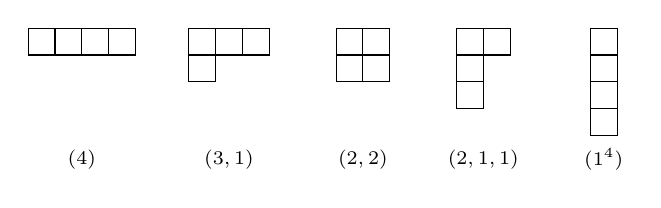
\begin{tikzpicture}[scale=0.34]
	\def\bx#1#2{\draw (#1,-#2) rectangle ++(1,1);}
	% (4)
	\begin{scope}[shift={(0,0)}]
		\foreach \c in {0,1,2,3} {\bx{\c}{0}}
		\node at (2,-3.9) {\scriptsize $(4)$};
	\end{scope}
	% (3,1)
	\begin{scope}[shift={(6,0)}]
		\foreach \c in {0,1,2} {\bx{\c}{0}}
		\bx{0}{1}
		\node at (1.5,-3.9) {\scriptsize $(3,1)$};
	\end{scope}
	% (2,2)
	\begin{scope}[shift={(11.5,0)}]
		\foreach \c in {0,1} {\bx{\c}{0}\bx{\c}{1}}
		\node at (1,-3.9) {\scriptsize $(2,2)$};
	\end{scope}
	% (2,1,1)
	\begin{scope}[shift={(16,0)}]
		\foreach \c in {0,1} {\bx{\c}{0}}
		\bx{0}{1}\bx{0}{2}
		\node at (1,-3.9) {\scriptsize $(2,1,1)$};
	\end{scope}
	% (1,1,1,1)
	\begin{scope}[shift={(21,0)}]
		\foreach \r in {0,1,2,3} {\bx{0}{\r}}
		\node at (0.5,-3.9) {\scriptsize $(1^4)$};
	\end{scope}
\end{tikzpicture}
\end{center}

and all the partitions of $5$:

\begin{center}
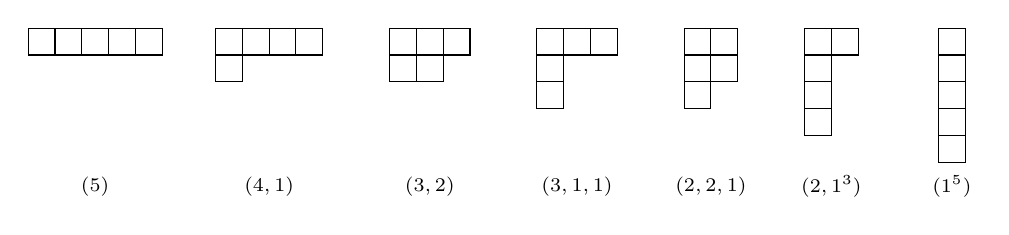
\begin{tikzpicture}[scale=0.34]
	\def\bx#1#2{\draw (#1,-#2) rectangle ++(1,1);}
	\begin{scope}[shift={(0,0)}]
		\foreach \c in {0,...,4} {\bx{\c}{0}}
		\node at (2.5,-4.9) {\scriptsize $(5)$};
	\end{scope}
	\begin{scope}[shift={(7,0)}]
		\foreach \c in {0,...,3} {\bx{\c}{0}}
		\bx{0}{1}
		\node at (2,-4.9) {\scriptsize $(4,1)$};
	\end{scope}
	\begin{scope}[shift={(13.5,0)}]
		\foreach \c in {0,1,2} {\bx{\c}{0}}
		\foreach \c in {0,1} {\bx{\c}{1}}
		\node at (1.5,-4.9) {\scriptsize $(3,2)$};
	\end{scope}
	\begin{scope}[shift={(19,0)}]
		\foreach \c in {0,1,2} {\bx{\c}{0}}
		\bx{0}{1}\bx{0}{2}
		\node at (1.5,-4.9) {\scriptsize $(3,1,1)$};
	\end{scope}
	\begin{scope}[shift={(24.5,0)}]
		\foreach \c in {0,1} {\bx{\c}{0}\bx{\c}{1}}
		\bx{0}{2}
		\node at (1,-4.9) {\scriptsize $(2,2,1)$};
	\end{scope}
	\begin{scope}[shift={(29,0)}]
		\foreach \c in {0,1} {\bx{\c}{0}}
		\bx{0}{1}\bx{0}{2}\bx{0}{3}
		\node at (1,-4.9) {\scriptsize $(2,1^3)$};
	\end{scope}
	\begin{scope}[shift={(34,0)}]
		\foreach \r in {0,...,4} {\bx{0}{\r}}
		\node at (0.5,-4.9) {\scriptsize $(1^5)$};
	\end{scope}
\end{tikzpicture}
\end{center}
\vspace{0.5em}

There are $p(4) = 5$ and $p(5) = 7$ of them, matching the five irreducible characters of $S_4$ and the seven of $S_5$ that we computed by hand.

\begin{definition}[Conjugate partition]
	The \vocab{conjugate} (or \vocab{transpose}) partition $\lambda'$ is obtained by reflecting the Young diagram in its main diagonal; that is, $\lambda_j' = \#\{i : \lambda_i \geq j\}$.
\end{definition}

For instance $(3,1)' = (2,1,1)$ and $(4,1)' = (2,1,1,1)$, while $(2,2)' = (2,2)$ and $(3,1,1)' = (3,1,1)$ are \vocab{self-conjugate}. Compare this with the tables we computed: the irreducible characters of $S_4$ and $S_5$ came in pairs swapped by tensoring with $\sign$, together with one or two fixed characters. That is exactly transposition of diagrams, as we now explain.

\subsection{Tableaux, Tabloids and Specht Modules}

\begin{definition}[Young tableau]
	A \vocab{($\lambda$-)tableau} is a filling of the Young diagram of $\lambda\vdash n$ with the numbers $1,\dots,n$, each used once. Two tableaux are \vocab{row equivalent} if corresponding rows contain the same sets of entries; an equivalence class is a \vocab{tabloid}, written $\{t\}$.
\end{definition}

The group $S_n$ acts on tableaux by acting on the entries, and this descends to an action on tabloids.

\begin{definition}[Permutation module]
	$M^\lambda$ is the permutation representation of $S_n$ on the set of $\lambda$-tabloids.
\end{definition}

\begin{example}
	If $\lambda = (n)$ there is a single tabloid, and $M^{(n)}$ is the trivial representation. If $\lambda = (1^n)$ a tabloid is just an ordering of $1,\dots,n$, so $M^{(1^n)} = \C S_n$ is the regular representation. If $\lambda = (n-1,1)$, a tabloid is determined by the entry in the second row, so $M^{(n-1,1)} = \C^n$ is the natural permutation representation.
\end{example}

These modules are far from irreducible, but each contains a distinguished irreducible submodule. Fix a $\lambda$-tableau $t$, and let
$$R_t = \{\sigma\in S_n : \sigma \text{ preserves each row of } t\}, \qquad C_t = \{\sigma\in S_n : \sigma\text{ preserves each column of } t\}$$
be its row and column groups.

\begin{definition}[Young symmetriser and Specht module]
	Define the \vocab{signed column sum} $b_t = \sum_{\sigma\in C_t}\sign(\sigma)\,\sigma \in \C S_n$, and the \vocab{polytabloid}
	$$e_t = b_t\cdot\{t\} \in M^\lambda.$$
	The \vocab{Specht module} is
	$$S^\lambda = \C S_n\text{-span of } \{e_t : t \text{ a }\lambda\text{-tableau}\} \; \leq \; M^\lambda.$$
\end{definition}

Since $\sigma e_t = e_{\sigma t}$, the span of the polytabloids is automatically a submodule.

\begin{theorem}[James]
	The Specht modules $S^\lambda$, for $\lambda\vdash n$, are irreducible, pairwise non-isomorphic, and every irreducible complex representation of $S_n$ is isomorphic to exactly one of them. Moreover
	$$S^{\lambda'} \cong S^\lambda\otimes\sign.$$
\end{theorem}

We do not prove this here -- the proof rests on a combinatorial lemma about tableaux (`if $\lambda \neq \mu$ and $b_t\cdot\{s\}\neq 0$ then $\lambda$ dominates $\mu$') together with an application of Schur's lemma. What matters for us is that the parametrisation exists and that we can compute with it. In particular, since transposing partitions is an involution on $\{\lambda\vdash n\}$ with fixed points the self-conjugate partitions, the last statement explains the pairing we observed.

\begin{proposition}[Hook length formula, Frame--Robinson--Thrall]
	For a box $(i,j)$ of the diagram of $\lambda$, define its \vocab{hook length} $h(i,j)$ to be $1$ plus the number of boxes strictly to its right in row $i$ plus the number strictly below it in column $j$. Then
	$$\dim S^\lambda = \frac{n!}{\prod_{(i,j)\in\lambda}h(i,j)}.$$
\end{proposition}

\begin{example}[The irreducibles of $S_4$]
	Let us compute the degrees. For $\lambda = (3,1)$ the hook lengths are
	\begin{center}
	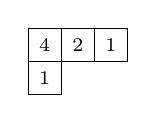
\begin{tikzpicture}[scale=0.42]
		\foreach \c/\v in {0/4, 1/2, 2/1} {\draw (\c,0) rectangle ++(1,1); \node at (\c+0.5,0.5) {\scriptsize $\v$};}
		\draw (0,-1) rectangle ++(1,1); \node at (0.5,-0.5) {\scriptsize $1$};
	\end{tikzpicture}
	\end{center}
	so $\dim S^{(3,1)} = 24/(4\cdot2\cdot1\cdot1) = 3$. Similarly $\dim S^{(2,2)} = 24/(3\cdot2\cdot2\cdot1) = 2$, and $\dim S^{(4)} = \dim S^{(1^4)} = 1$, with $\dim S^{(2,1,1)} = \dim S^{(3,1)} = 3$ by transposition. So the degrees are
	$$1,\; 3,\; 2,\; 3,\; 1 \qquad\text{with}\qquad 1+9+4+9+1 = 24 = |S_4|,$$
	exactly the degrees we found. Matching up: $S^{(4)} = \mathbf 1$, $S^{(1^4)} = \sign$, $S^{(3,1)}$ is the standard representation, $S^{(2,1,1)} = $ standard $\otimes\,\sign$, and $S^{(2,2)}$ is the degree-$2$ representation lifted from $S_4/V_4\cong S_3$.
\end{example}

\begin{example}[The irreducibles of $S_5$]
	The hook length formula gives
	$$\dim S^{(5)} = 1,\quad \dim S^{(4,1)} = \tfrac{120}{5\cdot3\cdot2\cdot1\cdot1} = 4,\quad \dim S^{(3,2)} = \tfrac{120}{4\cdot3\cdot1\cdot2\cdot1} = 5,\quad \dim S^{(3,1,1)} = \tfrac{120}{5\cdot2\cdot1\cdot2\cdot1} = 6,$$
	and the remaining three by transposition: $\dim S^{(2,2,1)} = 5$, $\dim S^{(2,1^3)} = 4$, $\dim S^{(1^5)} = 1$. The squares sum to
	$$1 + 16+25+36+25+16+1 = 120 = |S_5|.\ \checkmark$$
	Comparing with our computed table: $\lambda = (4,1)$ gives $\chi_3$ (degree $4$), $(2,1^3)$ gives $\chi_4 = \sign\cdot\chi_3$; $(3,2)$ gives $\chi_6$ (degree $5$) and $(2,2,1)$ gives $\chi_7$; and $(3,1,1)$, which is self-conjugate, gives the degree-$6$ character $\chi_5 = \Lambda^2\chi_3$. That is exactly the pattern of associate pairs and one self-associate character that we noticed at the time.
\end{example}

\begin{remark}
	There is also a combinatorial rule -- the Murnaghan--Nakayama rule -- computing the value of $\chi^\lambda$ on a permutation of cycle type $\mu$, by removing `rim hooks' from the diagram of $\lambda$. It is the natural generalisation of the recursion one finds by hand for small $n$. The interested reader will find all of this in James' book \emph{The Representation Theory of the Symmetric Groups}; for this course, the existence of the parametrisation and the hook length formula are the takeaway.
\end{remark}

\section{Representations of Topological Groups}

Everything so far has used the finiteness of $G$ in one essential place: the averaging operator $\frac1{|G|}\sum_{g\in G}$. If we can replace that sum by an integral, the entire theory goes through. This is possible exactly when $G$ is a compact topological group, and the resulting theory is one of the most useful things in mathematics -- it is, among other things, where the quantum mechanics of angular momentum comes from.

\subsection{Topological Groups and Compactness}

\begin{definition}[Topological group]
	A \vocab{topological group} is a group $G$ with a topology such that multiplication $G\times G\to G$ and inversion $G\to G$ are continuous.
\end{definition}

\begin{example}
	\begin{enumerate}[label=(\roman*)]
		\item Any group with the discrete topology; in particular any finite group.
		\item $(\R,+)$, $(\C^\times,\times)$, and $\GL_n(\C)$ with the topology inherited from $\C^{n^2}$.
		\item The compact groups $\OO(n)$, $\SO(n)$, $\U(n)$, $\SU(n)$, and the circle $S^1 = \{z\in\C : |z| = 1\} \cong \U(1)$.
	\end{enumerate}
	Of these, the ones in (iii) together with the finite groups are compact; $\R$, $\C^\times$ and $\GL_n(\C)$ are not.
\end{example}

\begin{definition}[Continuous representation]
	A \vocab{representation} of a topological group $G$ is a continuous homomorphism $\rho : G \to \GL(V)$ for a finite dimensional complex vector space $V$, where $\GL(V)$ has its usual topology. (Equivalently, all the matrix entries $\rho(g)_{ij}$ are continuous functions of $g$.)
\end{definition}

The continuity requirement is not a formality. The circle $S^1$ has uncountably many one-dimensional representations as an abstract group -- it is a divisible abelian group, so has vast numbers of homomorphisms to $\C^\times$ -- but only countably many continuous ones, as we shall see.

The replacement for averaging is the following.

\begin{definition}[Haar measure]
	Let $G$ be a compact topological group. A \vocab{Haar integral} on $G$ is a linear functional $f\mapsto\int_Gf$ on the space $C(G,\R)$ of continuous real functions such that
	\begin{enumerate}[label=(\roman*)]
		\item $\int_G 1 = 1$ (normalisation);
		\item $\int_G f(xg)\dd g = \int_G f(gx)\dd g = \int_G f(g)\dd g$ for all $x\in G$ (translation invariance);
		\item $\int_G f \geq 0$ whenever $f\geq0$ (positivity).
	\end{enumerate}
\end{definition}

\begin{theorem}
	Every compact Hausdorff topological group admits a unique Haar integral.
\end{theorem}

We shall not prove this -- it is a piece of analysis rather than algebra, and for the two groups we care about we can just write the integral down.

\begin{example}
	\begin{enumerate}[label=(\roman*)]
		\item If $G$ is finite, $\int_Gf = \frac1{|G|}\sum_{g\in G}f(g)$.
		\item If $G = S^1$, $\displaystyle\int_Gf = \frac1{2\pi}\int_0^{2\pi}f(e^{i\theta})\dd\theta$.
		\item If $G = \SU(2)$, which we will see is the unit sphere $S^3\subset\R^4$, the Haar integral is $\frac{1}{2\pi^2}$ times the usual surface integral over $S^3$ (and $2\pi^2$ is exactly the surface area of the unit $3$-sphere).
	\end{enumerate}
\end{example}

With the Haar integral in hand, the finite theory transfers essentially verbatim. We record what survives.

\begin{theorem}
	Let $G$ be a compact Hausdorff topological group and let $V, W$ be (continuous, finite dimensional, complex) representations of $G$. Then:
	\begin{enumerate}[label=(\roman*)]
		\item $V$ admits a $G$-invariant Hermitian inner product; equivalently $\rho(G)\leq\U(V)$ in a suitable basis.
		\item (Maschke) Every subrepresentation of $V$ has a $G$-invariant complement, so $V$ is completely reducible.
		\item (Schur) $\dim\Hom_G(V,W) = 1$ if $V\cong W$ are irreducible and $0$ if they are non-isomorphic irreducibles.
		\item (Orthogonality) With $\ip{f}{f'} = \int_G\overline{f(g)}f'(g)\dd g$, the irreducible characters are orthonormal; a representation is irreducible if and only if $\ip{\chi}{\chi} = 1$; and characters determine representations up to isomorphism.
	\end{enumerate}
\end{theorem}
\begin{proof}
	For (i), start from any inner product $(\cdot,\cdot)$ and set $\ip vw = \int_G(gv,gw)\dd g$, which converges since $g\mapsto (gv,gw)$ is continuous on a compact space; invariance is property (ii) of the Haar integral, and positive definiteness follows from (iii) together with $\int_G1 = 1$. Then (ii) follows by taking orthogonal complements, exactly as in the finite case. The proof of (iii) never used finiteness, only that $V$ is a finite dimensional complex vector space.

	For (iv), the proof of orthogonality goes through word for word: the map $\pi = \int_G\rho(g)\dd g$ is a projection onto $V^G$ with $\dim V^G = \int_G\chi_V$, the space $\Hom_\C(V,W)$ is a representation with $\Hom_\C(V,W)^G = \Hom_G(V,W)$ and character $\overline{\chi_V}\chi_W$, and combining gives $\ip{\chi_V}{\chi_W} = \dim\Hom_G(V,W)$. Schur finishes it.
\end{proof}

\begin{remark}
	One thing does \emph{not} transfer: a compact group generally has infinitely many irreducible representations, so there is no finite `character table' and no statement that $\sum d_i^2 = |G|$. The Peter--Weyl theorem is the correct replacement: the matrix coefficients of the irreducible representations span a dense subspace of $C(G)$, and $L^2(G)$ decomposes as $\widehat\bigoplus_i V_i^{\oplus d_i}$. For $G = S^1$ this is precisely the theory of Fourier series.
\end{remark}

\subsection{Representations of the Circle}

\begin{theorem}
	Every irreducible representation of $S^1$ is one dimensional, of the form $\rho_n : z\mapsto z^n$ for a unique $n\in\Z$.
\end{theorem}
\begin{proof}
	Since $S^1$ is abelian, Schur's lemma gives that every irreducible representation is one dimensional (the argument is identical to the finite case). So let $\rho : S^1\to\C^\times$ be a continuous homomorphism. The image $\rho(S^1)$ is a compact subgroup of $\C^\times$, hence bounded, and closed under taking powers; a complex number $\lambda$ with $|\lambda|\neq1$ has $|\lambda^n|\to\infty$ or $\to0$, so $\rho(S^1)\subseteq S^1$.

	Now consider $\psi : \R\to S^1$, $\psi(x) = \rho(e^{2\pi i x})$, a continuous homomorphism from $(\R,+)$. Lifting through the covering $\R\to S^1$ (or, concretely, choosing a continuous branch of $\frac{1}{2\pi i}\log\psi$ near $0$ and extending by additivity) gives a continuous homomorphism $\alpha : \R\to\R$ with $\psi(x) = e^{2\pi i\alpha(x)}$. A continuous additive map $\R\to\R$ is $x\mapsto\lambda x$: indeed $\alpha(q) = q\alpha(1)$ for $q\in\Q$ by additivity, and continuity extends this to $\R$. Finally $\psi(1) = \rho(1) = 1$ forces $\lambda = \alpha(1)\in\Z$, and then $\rho(z) = z^\lambda$.
\end{proof}

So the characters of $S^1$ are $\chi_n(e^{i\theta}) = e^{in\theta}$, and orthonormality reads
$$\frac1{2\pi}\int_0^{2\pi}e^{-im\theta}e^{in\theta}\dd\theta = \delta_{mn},$$
which the reader will recognise. Decomposing a representation of $S^1$ into irreducibles is decomposing a function into its Fourier modes; the Peter--Weyl theorem for $S^1$ is the completeness of the Fourier basis in $L^2(S^1)$.

\subsection{The Group \texorpdfstring{$\SU(2)$}{SU(2)}}

\begin{definition}
	$\SU(2) = \{A\in\GL_2(\C) : \overline A^{\,T}A = I,\ \det A = 1\}$.
\end{definition}

\begin{proposition}
	$$\SU(2) = \left\{\begin{pmatrix}a & b\\ -\overline b & \overline a\end{pmatrix} : a,b\in\C,\ |a|^2+|b|^2 = 1\right\},$$
	and hence $\SU(2)$ is homeomorphic to the unit sphere $S^3\subseteq\C^2 = \R^4$. In particular it is compact and connected.
\end{proposition}
\begin{proof}
	If $A = \left(\begin{smallmatrix}a&b\\c&d\end{smallmatrix}\right)$ has determinant $1$ then $A^{-1} = \left(\begin{smallmatrix}d&-b\\-c&a\end{smallmatrix}\right)$, and unitarity says $A^{-1} = \overline A^{\,T} = \left(\begin{smallmatrix}\overline a&\overline c\\ \overline b&\overline d\end{smallmatrix}\right)$. Comparing entries gives $d = \overline a$ and $c = -\overline b$, and then $\det A = |a|^2+|b|^2 = 1$. Conversely all such matrices are in $\SU(2)$.
\end{proof}

\begin{remark}
	Equivalently, $\SU(2)$ is the group of unit quaternions: identifying $\HH = \R\gen{1,i,j,k}$ with the set of matrices $\left(\begin{smallmatrix}a&b\\-\overline b&\overline a\end{smallmatrix}\right)$ (no norm condition), the quaternion norm is $\det$, and the unit quaternions are exactly $\SU(2)$. This is why $Q_8\leq\SU(2)$, and it is the source of the degree-$2$ representation of $Q_8$ we met earlier.
\end{remark}

The key to everything is the \vocab{maximal torus}
$$T = \left\{ t_\theta := \begin{pmatrix}e^{i\theta}&0\\0&e^{-i\theta}\end{pmatrix} : \theta\in\R\right\} \cong S^1 \; \leq \; \SU(2).$$

\begin{proposition}
	Every element of $\SU(2)$ is conjugate to some $t_\theta \in T$, and $t_\theta$ is conjugate to $t_{\theta'}$ if and only if $\theta' \equiv\pm\theta$. Consequently the conjugacy classes of $\SU(2)$ are in bijection with $[-1,1]$, via $A\mapsto\frac12\tr A = \cos\theta$.
\end{proposition}
\begin{proof}
	A unitary matrix is diagonalisable by a unitary change of basis (the spectral theorem from \emph{Linear Algebra}), so $A = PDP^{-1}$ with $P\in\U(2)$ and $D$ diagonal unitary. Since $\det A = 1$ the diagonal entries are $e^{\pm i\theta}$, so $D\in T$. Replacing $P$ by $\lambda^{-1}P$ where $\lambda^2 = \det P$ gives $P\in\SU(2)$ without changing $PDP^{-1}$.

	Now let $s = \left(\begin{smallmatrix}0&1\\-1&0\end{smallmatrix}\right)\in\SU(2)$. A direct computation gives $st_\theta s^{-1} = t_{-\theta}$, so $t_\theta\sim t_{-\theta}$. Conversely conjugate matrices have the same eigenvalues, so $t_\theta\sim t_{\theta'}$ forces $\{e^{i\theta},e^{-i\theta}\} = \{e^{i\theta'},e^{-i\theta'}\}$. Finally $\tr t_\theta = 2\cos\theta$ determines $\{\pm\theta\}$ modulo $2\pi$.
\end{proof}

The picture is worth having. Think of $\SU(2) = S^3$ as a sphere with poles $I$ and $-I$: the conjugacy classes are the `latitudes', which are honest $2$-spheres of radius $\sqrt{1-x^2}$ where $x = \frac12\tr$, degenerating to points at the poles. The maximal torus is a great circle through both poles, meeting each latitude in exactly the two points $t_\theta$ and $t_\theta^{-1} = t_{-\theta}$.

\begin{center}
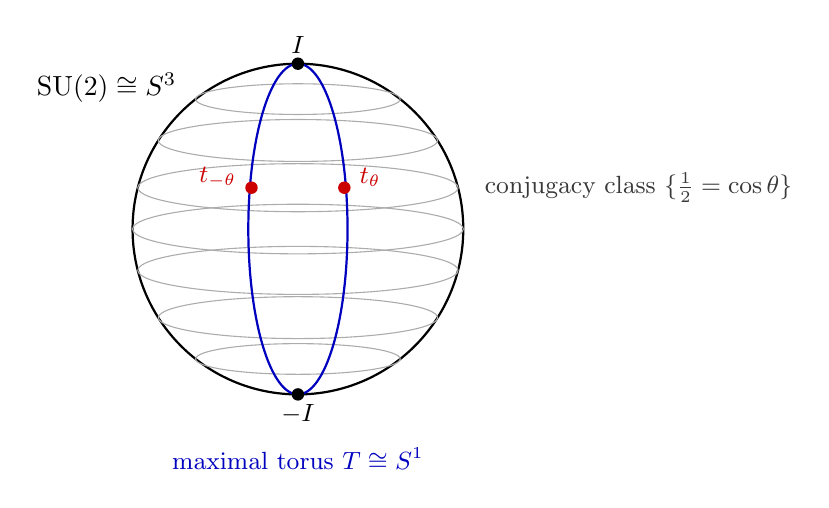
\begin{tikzpicture}[scale=1.5]
	\draw[thick] (0,0) circle (1.4);
	% latitudes (conjugacy classes)
	\foreach \y in {-1.1,-0.75,-0.35,0,0.35,0.75,1.1} {
		\pgfmathsetmacro{\rx}{sqrt(1.96-\y*\y)}
		\draw[gray!65] (0,\y) ellipse ({\rx} and {0.15*\rx});
	}
	% maximal torus: great circle through poles
	\draw[thick, color=blue!75!black] (0,0) ellipse (0.42 and 1.4);
	\fill (0,1.4) circle (1.5pt) node[above] {\small $I$};
	\fill (0,-1.4) circle (1.5pt) node[below] {\small $-I$};
	% intersection points on the latitude y = 0.35
	\fill[color=red!80!black] (0.393,0.35) circle (1.5pt);
	\fill[color=red!80!black] (-0.393,0.35) circle (1.5pt);
	\node[color=red!80!black, right] at (0.44,0.44) {\small $t_\theta$};
	\node[color=red!80!black, left] at (-0.44,0.44) {\small $t_{-\theta}$};
	\node[color=blue!75!black] at (0,-1.95) {\small maximal torus $T\cong S^1$};
	\node[color=gray!45!black, right] at (1.5,0.35) {\small conjugacy class $\{\tfrac12\tr = \cos\theta\}$};
	\node at (-1.62,1.2) {$\SU(2)\cong S^3$};
\end{tikzpicture}
\end{center}
\vspace{0.4em}

\begin{corollary}
	A class function on $\SU(2)$ is determined by its restriction to $T$, and that restriction satisfies $f(t_\theta) = f(t_{-\theta})$.
\end{corollary}

Integration of class functions can be pushed down to $T$ as well; the resulting formula is the simplest instance of the \emph{Weyl integration formula}.

\begin{proposition}[Weyl integration formula for $\SU(2)$]
	For a continuous class function $f$ on $\SU(2)$,
	$$\int_{\SU(2)}f = \frac2\pi\int_0^\pi f(t_\theta)\,\sin^2\theta\dd\theta.$$
\end{proposition}
\begin{proof}[Sketch]
	Under $\SU(2)\cong S^3$, the conjugacy class with $\frac12\tr = \cos\theta$ is the $2$-sphere of radius $\sin\theta$ obtained by intersecting $S^3$ with the hyperplane at height $\cos\theta$; its surface area is $4\pi\sin^2\theta$. Slicing $S^3$ by these spheres and using $\int_{\SU(2)}f = \frac1{2\pi^2}\int_{S^3}f$,
	$$\int_{\SU(2)}f = \frac1{2\pi^2}\int_0^\pi f(t_\theta)\cdot4\pi\sin^2\theta\dd\theta = \frac2\pi\int_0^\pi f(t_\theta)\sin^2\theta\dd\theta. \qedhere$$
\end{proof}

\subsection{The Irreducible Representations of \texorpdfstring{$\SU(2)$}{SU(2)}}

\begin{definition}
	Let $V_n$ be the space of homogeneous polynomials of degree $n$ in two variables $X, Y$ over $\C$:
	$$V_n = \C\gen{X^n,\ X^{n-1}Y,\ \dots,\ Y^n}, \qquad \dim V_n = n+1.$$
	Let $\GL_2(\C)$ -- and hence $\SU(2)$ -- act by
	$$\begin{pmatrix}a&b\\c&d\end{pmatrix}\cdot f(X,Y) = f(aX+cY,\ bX+dY).$$
\end{definition}

One checks this is a (continuous, polynomial in the entries) representation. Note $V_0$ is the trivial representation, $V_1$ is the standard representation on $\C^2$, and in general $V_n\cong S^nV_1$.

\begin{proposition}
	The character of $V_n$ satisfies
	$$\chi_n(t_\theta) = e^{in\theta}+e^{i(n-2)\theta}+\cdots+e^{-in\theta} = \frac{\sin\big((n+1)\theta\big)}{\sin\theta}.$$
\end{proposition}
\begin{proof}
	With $z = e^{i\theta}$ we have $t_\theta\cdot X = zX$ and $t_\theta\cdot Y = z^{-1}Y$, so
	$$t_\theta\cdot(X^jY^{n-j}) = z^{j}z^{-(n-j)}X^jY^{n-j} = z^{2j-n}X^jY^{n-j}.$$
	So the monomials are an eigenbasis with eigenvalues $z^{2j-n}$ for $j = 0,\dots,n$, and summing the geometric series gives $\sum_{j=0}^nz^{2j-n} = \frac{z^{n+1}-z^{-(n+1)}}{z-z^{-1}}$, which is $\sin((n+1)\theta)/\sin\theta$.
\end{proof}

\begin{theorem}
	Each $V_n$ is an irreducible representation of $\SU(2)$.
\end{theorem}
\begin{proof}
	First, a direct computation: $\ip{\chi_n}{\chi_n} = \frac2\pi\int_0^\pi\left|\frac{\sin((n+1)\theta)}{\sin\theta}\right|^2\sin^2\theta\dd\theta = \frac2\pi\int_0^\pi\sin^2\big((n+1)\theta\big)\dd\theta = \frac2\pi\cdot\frac\pi2 = 1$, so $V_n$ is irreducible.

	It is instructive to see this without integration. Let $0\neq W\leq V_n$ be $\SU(2)$-invariant. Then $W$ is $T$-invariant, and the monomials $X^jY^{n-j}$ span the $T$-eigenspaces, which are one dimensional with \emph{distinct} eigenvalues $z^{2j-n}$. Hence $W$ is spanned by a subset of the monomials. Pick $X^jY^{n-j}\in W$ and apply
	$$g = \frac1{\sqrt2}\begin{pmatrix}1&-1\\1&1\end{pmatrix}\in\SU(2),$$
	which sends $X\mapsto\frac{1}{\sqrt2}(X+Y)$ and $Y\mapsto\frac1{\sqrt2}(-X+Y)$. Then
	$$g\cdot(X^jY^{n-j}) = 2^{-n/2}(X+Y)^j(-X+Y)^{n-j}\in W$$
	has nonzero coefficient of $X^n$, namely $\pm2^{-n/2}$; since $W$ is spanned by monomials, $X^n\in W$. Applying $g$ again, $2^{-n/2}(X+Y)^n\in W$ has \emph{every} monomial coefficient nonzero, so every $X^jY^{n-j}$ lies in $W$ and $W = V_n$.
\end{proof}

\begin{theorem}
	Every irreducible representation of $\SU(2)$ is isomorphic to $V_n$ for exactly one $n\geq0$.
\end{theorem}
\begin{proof}
	Let $V$ be an irreducible representation with character $\chi$. Restricting $V$ to $T\cong S^1$ and decomposing into the characters $z\mapsto z^m$ of the circle, we get
	$$\chi(t_\theta) = \sum_{m\in\Z}a_mz^m, \qquad z = e^{i\theta},$$
	a Laurent polynomial with $a_m\in\Z_{\geq0}$ and only finitely many nonzero. Since $t_\theta$ and $t_{-\theta}$ are conjugate in $\SU(2)$, we have $a_m = a_{-m}$: the Laurent polynomial is symmetric under $z\mapsto z^{-1}$.

	Now the functions $\chi_n|_T = z^n+z^{n-2}+\cdots+z^{-n}$, for $n\geq 0$, form a $\Z$-basis of the group of symmetric Laurent polynomials with integer coefficients: they are `triangular', in that $\chi_n$ has top term $z^n$ with coefficient $1$. So we may subtract off successively and write
	$$\chi = \sum_{n\geq0}c_n\chi_n, \qquad c_n\in\Z,$$
	with only finitely many $c_n\neq0$. But then $1 = \ip\chi\chi = \sum_nc_n^2$ by orthonormality of the $\chi_n$, so exactly one $c_n$ is $\pm1$ and the rest are zero. As $\chi(1) > 0$ the sign is $+$, so $\chi = \chi_n$ and hence $V\cong V_n$.
\end{proof}

\subsection{The Clebsch--Gordan Formula}

Tensor products of the $V_n$ decompose in a completely explicit way. This is the mathematics behind `adding angular momenta' in quantum mechanics.

\begin{theorem}[Clebsch--Gordan]
	For $m, n\geq0$,
	$$V_m\otimes V_n \; \cong \; V_{m+n}\oplus V_{m+n-2}\oplus\cdots\oplus V_{|m-n|}.$$
\end{theorem}
\begin{proof}
	Assume without loss of generality that $m\leq n$. Work on $T$, writing $z = e^{i\theta}$, and clear the denominator: multiplying by $z - z^{-1}$,
	$$\chi_m\chi_n\cdot(z-z^{-1}) = \Big(\sum_{j=0}^mz^{m-2j}\Big)\big(z^{n+1}-z^{-(n+1)}\big) = \sum_{j=0}^m z^{m+n+1-2j} \; - \; \sum_{j=0}^mz^{m-n-1-2j}.$$
	On the other hand,
	$$\Big(\sum_{j=0}^m\chi_{m+n-2j}\Big)(z-z^{-1}) = \sum_{j=0}^m z^{m+n+1-2j} \; - \; \sum_{j=0}^m z^{-(m+n+1-2j)}.$$
	The first sums are literally equal. For the second sums, as $j$ runs from $0$ to $m$ the exponents $m-n-1-2j$ run through
	$$m-n-1,\ m-n-3,\ \dots,\ -m-n-1,$$
	while the exponents $-(m+n+1-2j)$ run through the same list in the opposite order. So the two expressions agree, and since $z - z^{-1}$ is not identically zero we get $\chi_m\chi_n = \sum_{j=0}^m\chi_{m+n-2j}$ on $T$, hence everywhere. As characters determine representations, the decomposition follows.
\end{proof}

The bookkeeping is clearest as a picture. The $T$-weights of $V_m\otimes V_n$ are the sums of a weight of $V_m$ and a weight of $V_n$, so they form a rectangular grid, and the multiplicity of a given weight is the number of lattice points on the corresponding anti-diagonal. Reading off the multiplicity profile and peeling off one layer at a time gives the decomposition. For $V_2\otimes V_3$:

\begin{center}
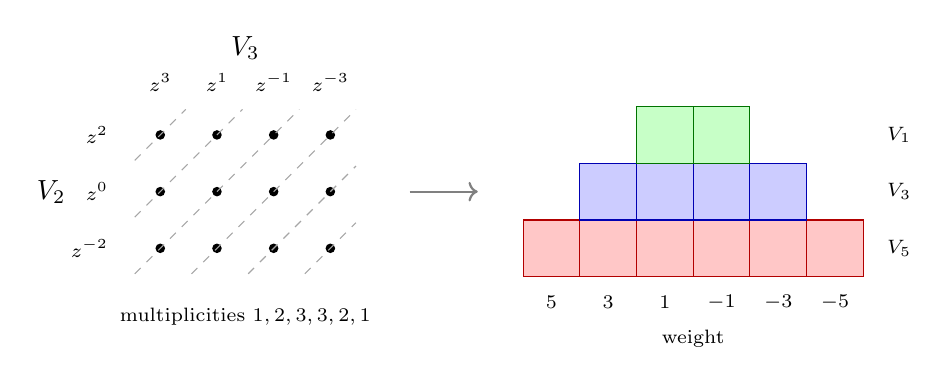
\begin{tikzpicture}[scale=0.72]
	% left: grid of weights
	\foreach \i in {0,1,2} {
		\foreach \j in {0,1,2,3} {
			\fill[black] (\j,-\i) circle (2.4pt);
		}
	}
	\foreach \d in {0,...,5} {
		\draw[gray!70, dashed] ({max(0,\d-2)-0.45},{-min(2,\d)-0.45}) -- ({min(3,\d)+0.45},{-max(0,\d-3)+0.45});
	}
	\node[left] at (-0.75,0) {\scriptsize $z^{2}$};
	\node[left] at (-0.75,-1) {\scriptsize $z^{0}$};
	\node[left] at (-0.75,-2) {\scriptsize $z^{-2}$};
	\node[above] at (0,0.6) {\scriptsize $z^{3}$};
	\node[above] at (1,0.6) {\scriptsize $z^{1}$};
	\node[above] at (2,0.6) {\scriptsize $z^{-1}$};
	\node[above] at (3,0.6) {\scriptsize $z^{-3}$};
	\node[left] at (-1.5,-1) {$V_2$};
	\node[above] at (1.5,1.15) {$V_3$};
	\node at (1.5,-3.2) {\scriptsize multiplicities $1,2,3,3,2,1$};
	% arrow
	\draw[->, thick, gray] (4.4,-1) -- (5.6,-1);
	% right: stacked layers
	\begin{scope}[shift={(6.4,0)}]
		\foreach \x in {0,...,5} {\draw[fill=red!22, draw=red!70!black] (\x,-2.5) rectangle ++(1,1);}
		\foreach \x in {1,...,4} {\draw[fill=blue!20, draw=blue!70!black] (\x,-1.5) rectangle ++(1,1);}
		\foreach \x in {2,3} {\draw[fill=green!22, draw=green!45!black] (\x,-0.5) rectangle ++(1,1);}
		\node[right] at (6.25,-2) {\scriptsize $V_5$};
		\node[right] at (6.25,-1) {\scriptsize $V_3$};
		\node[right] at (6.25,0) {\scriptsize $V_1$};
		\foreach \x/\w in {0/5, 1/3, 2/1, 3/{-1}, 4/{-3}, 5/{-5}} {
			\node at (\x+0.5,-2.95) {\scriptsize $\w$};
		}
		\node at (3,-3.6) {\scriptsize weight};
	\end{scope}
\end{tikzpicture}
\end{center}
\vspace{0.3em}
so $V_2\otimes V_3\cong V_5\oplus V_3\oplus V_1$, as the theorem predicts.

\begin{example}
	$V_1\otimes V_1\cong V_2\oplus V_0$: the tensor square of the standard $2$-dimensional representation splits as $S^2V_1\oplus\Lambda^2V_1$, and indeed $S^2V_1 = V_2$ while $\Lambda^2V_1$ is one dimensional with trivial action (as $\det = 1$ on $\SU(2)$).
\end{example}

\subsection{From \texorpdfstring{$\SU(2)$}{SU(2)} to \texorpdfstring{$\SO(3)$}{SO(3)}}

\begin{theorem}
	There is a surjective continuous homomorphism $\varphi : \SU(2)\to\SO(3)$ with kernel $\{\pm I\}$, inducing an isomorphism of topological groups
	$$\SU(2)/\{\pm I\}\;\cong\;\SO(3).$$
\end{theorem}
\begin{proof}
	Let
	$$\mathfrak{su}(2) = \{A\in M_2(\C) : \overline A^{\,T} = -A,\ \tr A = 0\} = \R\gen{\begin{pmatrix}i&0\\0&-i\end{pmatrix},\begin{pmatrix}0&1\\-1&0\end{pmatrix},\begin{pmatrix}0&i\\i&0\end{pmatrix}},$$
	a real vector space of dimension $3$. (These are the `purely imaginary quaternions'.) Equip it with the inner product $\ip AB = \frac12\tr(A\overline B^{\,T})$, for which the displayed basis is orthonormal, and note $\ip AA = \det A$ for $A\in\mathfrak{su}(2)$.

	The group $\SU(2)$ acts on $\mathfrak{su}(2)$ by conjugation, $\varphi(g)(A) = gAg^{-1}$; this preserves trace and adjoints, so preserves $\mathfrak{su}(2)$, and it preserves $\det$, hence the inner product. So $\varphi : \SU(2)\to\OO(3)$ is a continuous homomorphism. Since $\SU(2)\cong S^3$ is connected and $\varphi(I) = I$, the image lies in the identity component $\SO(3)$.

	The kernel consists of those $g$ commuting with all of $\mathfrak{su}(2)$, hence with all of $M_2(\C)$ (which $\mathfrak{su}(2)$ spans over $\C$ together with $I$), hence the scalars in $\SU(2)$, which are $\pm I$.

	For surjectivity, compute: conjugation by $t_\theta$ fixes $\left(\begin{smallmatrix}i&0\\0&-i\end{smallmatrix}\right)$ and rotates the other two basis vectors by $2\theta$. So the image contains all rotations about one axis by all angles; and conjugating this one-parameter family by other elements of $\SU(2)$ -- whose image acts transitively on axes, since $\SU(2)$ acts transitively on the unit sphere of $\mathfrak{su}(2)$ -- gives all rotations. Hence $\varphi$ is onto. The induced bijection $\SU(2)/\{\pm I\}\to\SO(3)$ is a continuous bijection from a compact space to a Hausdorff space, hence a homeomorphism.
\end{proof}

So $\SU(2)$ is a \emph{double cover} of $\SO(3)$: each rotation has exactly two preimages, $\pm g$. Concretely, the rotation by angle $2\theta$ about a fixed axis is the image of both $t_\theta$ and $t_{\theta+\pi} = -t_\theta$; going once round a loop of rotations lifts to a path in $\SU(2)$ from $g$ to $-g$.

\begin{center}
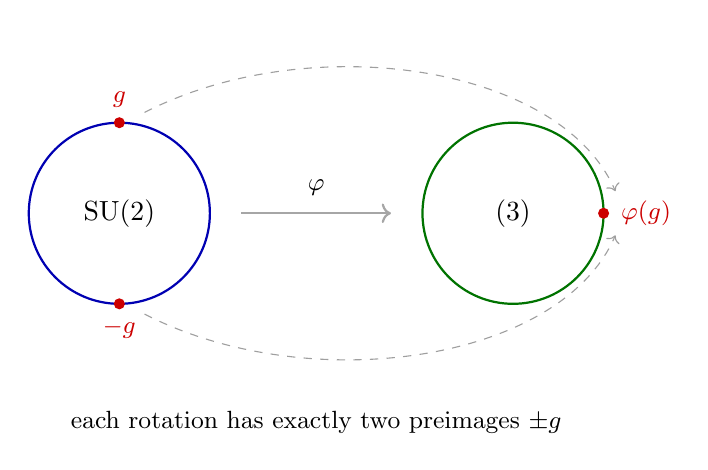
\begin{tikzpicture}[scale=1]
	\draw[thick, color=blue!70!black] (0,0) circle (1.15);
	\node at (0,0) {$\SU(2)$};
	\draw[thick, color=green!45!black] (5,0) circle (1.15);
	\node at (5,0) {$\SO(3)$};
	\fill[color=red!80!black] (0,1.15) circle (2pt);
	\fill[color=red!80!black] (0,-1.15) circle (2pt);
	\fill[color=red!80!black] (6.15,0) circle (2pt);
	\node[above, color=red!80!black] at (0,1.22) {\small $g$};
	\node[below, color=red!80!black] at (0,-1.22) {\small $-g$};
	\node[right, color=red!80!black] at (6.25,0) {\small $\varphi(g)$};
	\draw[->, thick, gray!70] (1.55,0) -- (3.45,0);
	\node[above] at (2.5,0.1) {\small $\varphi$};
	\draw[->, dashed, gray!75] (0.32,1.28) .. controls (2.4,2.35) and (5.6,1.9) .. (6.3,0.28);
	\draw[->, dashed, gray!75] (0.32,-1.28) .. controls (2.4,-2.35) and (5.6,-1.9) .. (6.3,-0.28);
	\node at (2.5,-2.65) {\small each rotation has exactly two preimages $\pm g$};
\end{tikzpicture}
\end{center}
\vspace{0.3em}

\begin{corollary}
	The irreducible representations of $\SO(3)$ are exactly the $V_{2n}$ for $n\geq0$, of odd dimensions $1, 3, 5,\dots$
\end{corollary}
\begin{proof}
	By the lifting correspondence, representations of $\SO(3) = \SU(2)/\{\pm I\}$ are precisely representations of $\SU(2)$ with $-I$ in the kernel, and irreducibility is preserved. Now $-I = t_\pi$ acts on $V_n$ with eigenvalues $(e^{i\pi})^{2j-n} = (-1)^n$, so $-I$ acts as $(-1)^n\id$. This is trivial exactly when $n$ is even.
\end{proof}

\begin{remark}
	This is why in quantum mechanics the orbital angular momentum states come in multiplets of odd dimension $2\ell+1$ (representations of the rotation group $\SO(3)$), while spin-$\frac12$ particles live in the even dimensional representations $V_{\text{odd}}$, which are representations of $\SU(2)$ but only \emph{projective} representations of $\SO(3)$: rotating a spin-$\frac12$ state by $2\pi$ multiplies it by $-1$. The Clebsch--Gordan formula, in the physicists' labelling $V_n \leftrightarrow$ spin $j = n/2$, reads
	$$j_1\otimes j_2 = (j_1+j_2)\oplus(j_1+j_2-1)\oplus\cdots\oplus|j_1-j_2|,$$
	which is the rule for adding angular momenta.
\end{remark}

\begin{example}[$\SO(3)$ and $\SU(2)$ inside $\U(2)$]
	One can push this further. Every element of $\U(2)$ is $\lambda A$ with $|\lambda| = 1$ and $A\in\SU(2)$, so there is a surjection $S^1\times\SU(2)\to\U(2)$ with kernel $\{(1,I),(-1,-I)\}$. Since the irreducible representations of a product are the tensor products of irreducibles, the irreducible representations of $\U(2)$ are the $\rho_m\otimes V_n$ with $m\equiv n\pmod 2$, i.e. $\det^{\,k}\otimes V_n$ for $k \in\Z$ and $n\geq0$.
\end{example}

\begin{remark}[What was left out]
	We have taken the shortest path to $\SU(2)$. The general theory of compact connected Lie groups -- maximal tori, roots and weights, the Weyl group, the Weyl character formula -- has $\SU(2)$ as its first and smallest case, and every feature we used (the torus $T$, the two-element Weyl group generated by $z\mapsto z^{-1}$, the factor $\sin^2\theta = |z - z^{-1}|^2/4$ in the integration formula, the triangular basis of characters) is an instance of a general phenomenon. That is the subject of a Part III course.
\end{remark}

\end{document}
